%PDF-методичка
%Версия 2.4 (для треда 21)
%In the name of the Goddess Aya Shameimaru, for teh great justice!

\documentclass[a4paper,14pt,oneside]{memoir}
\usepackage[russian]{babel}
\usepackage[utf8]{inputenc}
\usepackage{indentfirst}
\usepackage[scale=0.7]{geometry}
\usepackage{graphicx}
\usepackage{color}
\usepackage{tikz}
\usepackage{subfig}
\usepackage{caption}
\usepackage{url}
\usepackage{fix-cm}
\usepackage{pscyr}
\usepackage[pdfborder={0 0 0}, colorlinks=false, urlcolor=red]{hyperref}
\usepackage{memhfixc}



%\pdfinfo{
%/Author (dobrochan.ru)
%/Title (pdf-metodichka)
%}

\hypersetup{pdffitwindow=true}
\hypersetup{pdfmenubar=false}
\hypersetup{pdftitle={PDF-методичка}}
\hypersetup{pdfauthor={dobrochan.ru}}
\hypersetup{pdfsubject={Lucid dreaming}}
\hypersetup{pdfproducer={elbowfag}}

\captionsetup{font=small}
\captionsetup{font=sf}
\captionsetup{labelsep=none}

\definecolor{futabaheader}{RGB}{238,170,136} % тёмно-персиковый цвет задника
\definecolor{futababack}{RGB}{240,224,214} % фон постов
\definecolor{futabatext}{RGB}{96,0,0} % цвет текста на футабе
\definecolor{futabaq}{RGB}{120,153,34} % цвет цитат
\definecolor{shadecolor}{RGB}{229,229,229} % серая заливка кулстори

\graphicspath{{d:/metodichkae/}}

\chapterstyle{crosshead}

\clubpenalty=700
\widowpenalty=700

\urlstyle{sf}

\makepagestyle{conf}
 \makeevenfoot{conf}{}{lucid-dreaming@conference.jabber.ru}{}
 \makeoddfoot{conf}{}{Наша конференция в jabber:\\ lucid-dreaming@conference.jabber.ru}{}

\begin{document}

\begin{titlingpage}


\begin{center}
 \begin{Huge}
   \fontsize{45}{45}\selectfont Методичка\\ по осознанным \\сновидениям\\
	\end{Huge}

\vspace{0.7 cm}


\includegraphics[width=0.73\textwidth]{titleillst}

\vspace{0.4 cm}

\normalsize

\vspace {1.5cm}
\url{dobrochan.ru/u/}

{\small\sffamily 2012}

\end{center}

\end{titlingpage}


\thispagestyle{empty}

{\large\textsf{Вступление}}

\bigskip

\setcounter{page}{2}
Привет, анон. Перед тобой методичка по осознанным сновидениям, составленная сновидцами Доброчана за время существования треда. В ней содержатся теории, методики и просто различные мысли, так или иначе связанные со сновидческой практикой. Методичка формировалась прямо в процессе развития нашего сообщества, поэтому будет не лишним рассказать о том как всё начиналось и к чему в итоге пришло.

Итак, первый ОС-тред появился в /u/ниверситете в ноябре 2009 года. Как и все прочие стихийно возникающие на бордах треды, посвященные этой, скажем так, довольно скользкой теме, он не приобрёл особой популярности и не утонул только благодаря резиновому движку Доброчана. Тогда в треде не было ни практик, ни толковых советов для начинающего сновидца, поэтому новичкам, незнакомым с осознанными сновидениями, он и не был особо интересен. Но в июле 2010 в треде появился опытный сновидец,  теоретически подкованный и имевший за плечами несколько лет практики.  Ему удалось заинтересовать многих анонов темой осознанных сновидений, именно тогда формат треда и изменился, приобретая очертания того, каким он стал сейчас.



В первую очередь, был составлен FAQ для новичков, в котором понятным языком было объяснено, что и как должен делать начинающий сновидец, чтобы попасть в ОС. Во избежание ненужных срачей и набегов диванных теоретиков от эзотерики, в треде сразу было установлено правило, которого придерживаются и сейчас: <<Только научный подход @ Только практика>>. В результате в тред начали подтягиваться аноны, которых раньше отпугивали упоротые истории про летунов, светимость и прочий астрал. 


\thispagestyle{empty}




Более того, одной из главных идей треда постулировалась возможность целенаправленно влиять на свою психику с помощью осознанных сновидений, например, избавиться с их помощью от фобий, комплексов и прочих багов. Такой подход стал возможен, исходя из идеи о том, что сон~--- это продукт работы бессознательного, где хранятся все радости и печали человека. Для понимания психических процессов анонам было предложено вдумчиво курить Юнга, чтобы научиться понимать, куда в ОСе нужно тыкать для получения желаемого. Но всё это ещё было впереди, а пока начинающие сновидцы осваивали простенькие техники входа в ОС, учились запомнить сны и воспринимать их как важную часть своей жизни. Не прошло и месяца как будущие осозняши добились своих первых результатов,  и в треде начали появляться восторженные репорты, описывающие первые робкие попытки осознаться во сне.


Время шло, сновидцы Доброчана понемногу осваивали мир осознанных сновидений, успев обсудить множество возникающих у новичков вопросов и написать различные статьи, которые впоследствии и легли в основу этой методички. На определённом этапе, а именно в десятом треде,  все объёмные посты были собраны в один текстовый файл, чтобы отделить разросшийся FAQ от прочих мыслей, которые ОП-пост был уже не в состоянии вместить. Методичка периодически обновлялась новыми статьями и постами, но, представляя на тот момент довольно-таки хаотичный поток сознания, требовала серьёзной доработки редакторским напильником. К пятнадцатому треду силами осозняш методичка сменила формат на pdf, содержание было реструктурировано, а все тексты тщательно вычитаны и проверены сновидцами из числа граммар-наци. Наконец, в двадцатом треде была создана альтернативная версия для печати. В этой методичке есть море полезной информации, лишь бы у тебя, анон, было желание всё это читать.


\thispagestyle{empty}

За время своего существования ОС-тред несколько раз кардинально менялся, как и в любом сообществе,  были и вины, и драмы, но суть остаётся прежней: любой сновидец, как начинающий, так и продвинутый всё также может поделиться своими успехами и неудачами, задать вопросы и приобщиться к тёплой и ламповой атмосфере, по-прежнему хранимой и осозняшами, ещё в первых тредах открывшими для себя мир осознанных сновидений, и теми, кто присоединился к нам совсем недавно. 

\thispagestyle{empty}

Всё во имя того, чтобы зашедший на Доброчан сновидец не чувствовал себя одиноким. Главное~--- без фанатизма!

\clearpage
\tableofcontents


\part{Основы}

\chapter{FAQ}
\section{Введение}
Привет, анон, вот ты решил заняться осознанными сновидениями, давай сразу пробежимся по часто задаваемым вопросам.

\begin{center}
\textbf{<<А что это такое?>>}
\end{center}


Осознанные сны~--- это  сны, в которых ты осознал, что спишь, что дало тебе над ними контроль, возможность там делать всё, что пожелаешь.

\begin{center}
\bfseries{<<А нафига это надо?>>}
\end{center}


Во-первых, это весело, в хорошем осознанном сне ощущения зачастую даже ярче, чем IRL; там можно полетать, поебать тян (или кунов :3), полюбоваться на всякие интересные и/или красивые места и прочее.

Во-вторых, ITT мы используем подход ко снам, опираясь на Юнга, то есть сон~--- это не просто <<бред мозга>>, а продукт твоего бессознательного, там находятся твои проблемы, страхи, радости и печали. В конце концов, поведение, мысли и желания человека на 90\% определяются тем самым подсознанием. А осознанный сон даёт возможность по этому подсознанию погулять, причём~--- не просто погулять, но и исправить свои комплексы, фобии, страхи, а также лучше понять себя и ещё делать много-много других увлекательных вещей. 

\clearpage


\begin{center}
\bfseries{<<Это, наверное, сложно? Требует времени и превозмогания?>>}
\end{center}


Ничего сложного, основных упражнений вообще только два (о них ниже) и времени они занимают минут десять утром и минут пять в течение дня :3 

\begin{center}
\bfseries{<<А это не опасно? Вдруг я там, у себя в голове, что-нибудь поломаю?>>}
\end{center}


Нет, не опасно, что-то изменить в себе можно только осознанными действиями, IRL ты ведь не можешь себе <<случайно>> голову топором отрубить? Кроме того, у психики есть защита от <<криворукого пользователя>>, поэтому, если будешь делать что-то не так, то просто проснёшься. 


\begin{center}
\bfseries{<<Я слышал, что всё это эзотерические бредни, причём же тут наука?>>}
\end{center}


На самом деле, подходов к вопросу <<Что такое ОС?>> есть несколько.
 
Помимо всякой эзотерики, есть вполне себе научное его объяснение, которое уже достаточно давно признано на западе. <<Пробил>> его некто Стивен Лаберж, но о нём чуть ниже.
 
В этом треде мы придерживаемся ТОЛЬКО научного подхода, который опирается на следующие постулаты:
\begin{itemize}
\item Все сны и ОСы происходят только у тебя в голове. Никаких астралов, ВТО, менталов, параллельных миров и прочего. 
\item Все существа, люди, духи, НЁХ и прочие, кто встречается во сне~--- это всего лишь плод твоего бессознательного. Более подробно об этом чуть позже.
\end{itemize}

При этом считаю важным отметить, что, несмотря на такую категорическую позицию, к другим подходам мы относимся с уважением (Доброчан же!), что-то на уровне <<Мы вас понимаем, но сами считаем по-другому>>.


\section{Дневник снов}

Дневник снов~--- это, без преувеличения, самое важное на всех этапах работы с ОСами. Кроме того, ещё, пожалуй, и самое сложное, так как требует превозмогать по утрам свою лень (превозмогай лень@будь мужиком блеять).
Сразу отмечу, что если какие-то сны из детства ты и так помнишь~--- всё равно перенеси их в дневник, причём сразу. 

Дам некоторые рекомендации по его ведению. Во-первых, писать надо на бумаге; перед сном кладём тетрадь с ручкой около себя, и, как только просыпаемся, то сразу (СРАЗУ БЛДЖАД) записываем то, что помним, никаких там кофе, чистить зубы и т.д. Первым делом делаем запись. Если сон помнится обрывками, то можно немного полежать после пробуждения, не открывая глаз; не нужно пытаться вспомнить сон через силу и напряжение; часто бывает, что вот проснулся, помнишь момент сна, сразу вцепляешься в него зубами, а в результате~--- фейл. Оптимально будет поваляться в кровати, просто <<перекатывая>> в голове запомнившийся момент. В любом случае, важно записать хоть что-то. Если совсем ничего не вспоминается, то пиши, в каком настроении проснулся хотя бы.
Описывать надо как можно подробнее, помимо самого сюжета советую акцентировать внимание на:
\begin{itemize}
\item Местности (где происходило, что вокруг, что привлекло внимание, и т.д.).
\item Ощущениях (<<Почему-то от того небоскрёба мне захотелось посрать кирпичами>>).
\item Тому, как ты видел (чётко, размыто, в цвете или нет, и т.д.).
\item Сколько субъективно сон длился по времени.
\item Времени, когда лег спать и когда проснулся.
\item Дате сна.
\end{itemize}

Алсо, у многих бывает, что, на минуту проснувшись среди ночи, очень ярко помнишь, что снилось, но потом проскакивает мысль <<С утра запишу, это ведь невозможно забыть!>>, а наутро~--- конечно же, забыл. Фейл.

Логичный совет: записать хотя бы пару фраз из того, что помнишь, чтобы утром использовать их как ниточки для вытягивания всего сна. Но сказать это легко, а тянуться ночью к ручке с бумагой и что-то писать~--- это просто титаническое усилие. Можно схитрить, класть рядом ещё и диктофон, так как намного проще дотянуться до него рукой, нажать одну кнопку и проговорить 5--7 фраз о сне. Но наутро всё равно рекомендую перенести записи в дневник. Если и такой вариант не выходит, то можно купить диктофон, который включается от звука, и повесить его над кроватью (например, в сачке). Можно также в дневнике делать зарисовки (если умеешь рисовать) пейзажей и всяких других моментов сна.

Также важный момент, дневник должен нравиться тебе внешне, то есть, при взгляде на него должно хотеться сказать <<Ня!>>. Неважно, как он выглядит, главное~--- чтобы нравился именно тебе. Рекомендую походить по магазинам и выбрать себе добротную толстую записную книжку, которая вызовет восторг.

Теперь пара слов о том, как это работает.

Всё просто: дело в том, что все эти пляски с дневником прививают психике идею <<Надо, сцуко, сны запоминать>>\ldots Собственно, вот и весь его первый аспект :3 Подробное описание механизмов, я думаю, мало кому интересно; это я к тому, что тут чистая психология.

Второй момент~--- это, собственно, сами записи снов; периодическое их прочтение поможет растормошить <<сновидческую память>> (зона памяти, которая у нас частично блокирована), также записи понадобятся для другой практики (см.~ниже), ну и можно следить за своими успехами.

Вообще, рекомендую, если решил заниматься серьёзно, вести и обычный дневник, где нужно записывать кратко, что было в течение дня. Через месяц ведения записей можно, анализируя их, делать интересные выводы, например <<В дни, когда я ложился до 21 часа, сны запоминались очень ярко и чётко>>, или <<Пара ОСов была, когда я перед сном мешал пиво и вино>> :3. Это всё очень полезно, и данная информация лично мне приносит пользу и сейчас (после четырёх лет занятий).

Есть одно интересное упражнение, связанное с дневником снов (разработанное, кстати, аноном в прошлых тредах), суть такова: время от времени полезно переносить записи о плохо запомнившихся снах (а если не лень, то и остальных) из одного формата в другой, то есть, если писал на бумаге, то перепечатай в комп, если на компе\ldots Ну ты понел :3 Такое упражнение часто помогает вспомнить многие детали снов, а то и вообще целые забытые раньше сны.
 
Если ты сейчас подумал что-то из серии <<Да мне вообще сны не снятся!>>, то ты ошибаешься, снятся они всем и каждую ночь, просто ты их забываешь. Начни вести дневник, и уже через пару дней ты сильно удивишься результатам :3 

\section{Рука}

Также крайне простая и полезная практика на всех этапах.

Суть такова: в течение дня тебе надо проделывать следующий алгоритм действий (чем чаще будешь вспоминать, тем лучше, но без фанатизма):
\begin{itemize}
\item Задаёшься вопросом <<Сплю ли я?>>, желательно его проговорить про себя.
\item Смотришь на свою открытую ладонь, вглядываешься в чёрточки на руке и прочие её детали.
\item Начинаешь осматривать происходящее вокруг, при этом не фиксируешь внимание на чём-то одном, а быстро <<бегаешь>> взглядом по разным предметам, людям и т.д.
\end{itemize}

Тут есть ещё пара важных моментов. Во-первых~--- это не должно стать рутиной. Во-вторых~--- во время осмотра нужно как-то внутренне напрячься, это сложно описать, но нечто похожее происходит, когда ты в тишине слышишь какой-то резкий звук, в первый момент происходит внутреннее напряжение, вот что-то подобное и нужно.

Ещё годные примеры напряжения это: волнение перед экзаменом; перед первым поцелуем; собранность перед дракой; идешь по улице, и вдруг ХУЯК кирпич/сосулька прямо перед тобой падает.
 
Можно ещё поставить рандомный будильник на компе, чтобы он ВНЕЗАПНО издал громкий звук, в этот момент после отложения кирпичей ты пару мгновений будешь очень <<собран>>, вот это чувство тебе и нужно.

Всё <<действо>> должно занимать 10--20 секунд. Выполнять руку оптимально 8--12 раз в день, не нужно смотреть на неё каждые 10 минут, в таком случае пользы от упражнения не будет. Важно стараться вспоминать про руку во время разговора, чтения, просмотра кино и других действий, которые увлекают. 

Также полезно <<поощрять>> себя за это упражнение. Например, после каждого просмотра можно скушать маленький кусочек шоколадки :3
Всё, вот тебе самая эффективная практика на первых порах.

\smallskip
\fancybreak{* * *}

Теперь разберём, почему это работает.

Во сне мало задаться вопросом <<Сплю ли я?>>. Ты с чистой совестью можешь решить, что <<Не, нифига, не сплю>>, и сон продолжится. Важно именно посмотреть на свою ладонь. Почему ладонь? И почему это работает? Попробую вкратце объяснить:

Изначально возникает мысль <<Я что, сплю?>>/<<Это сон?>>/<<Что за бред?>>, и она нарушает структуру сна, привнося в неё сомнения, что логично приводит к пробуждению.

Что делает рука? На неё во время дневных упражнений вешается целый ряд рефлексов (концентрация, внутренняя собранность, бегание взгляда и т.д.). Соответственно, после вопроса сновидец и смотрит на руку, в результате в результате чего врубается этот рефлекторный психологический комплекс, а это приводит к увеличению стабильности и так далее.
Ладно\ldots{} Если провести аналогию, <<рука>>~--- это такой комплекс спеллов, привязанный на одну кнопку (тренировками в реале), за одно нажатие (во сне) твой перс сразу <<лечит>>, накидывает <<святой доспех>> и врубает <<ярость берсерка>> :3

Между прочим, эта техника взята из книги Кастенеды, что какбэ намекает нам, что, мол, полезно искать упражнения и в откровенно эзотерических источниках (шаманы пользуются ОСами, без преувеличений, тысячелетиями). И, если подойти к ним с умом, то станет понятно, что никакой <<мистики>> в них нет. 

Теперь на тему <<А можно, я буду тыкать пальцем в ладошку, смотреть на часы, пытаться взлететь, искать несоответствия во сне и т.д.>>: можно, конечно, но пользы, как правило, от таких упражнений немного; кроме того, как показывает опыт, лучше больше одного-двух упражнений не задрачивать. Рука обязательна в любом случае. Ну, можете что-то ещё взять, хотя лично я первое время рекомендую ограничиться только ей (ну и дневник, конечно).

Собственно, из базовых вещей~--- ВСЁ. Этих двух практик вполне хватит, чтобы добиться первого ОСа за недели две-три. Да и дальнейшее их надрачивание будет полезно.
Так что рекомендую вновь прибывшим первым делом хотя бы две недели позаниматься по этим упражнениям (их вообще хорошо делать всю жизнь), а уже потом, исходя из результатов, хвататься за остальное предложенное в методичке. 

И кстати вот ещё: при записи текста в дневник, каждый раз делай вначале проверку руки. Многим после начала практик начинает сниться, что они просыпаются и начинают записывать свой сон\ldots Ну, думаю, ты уже понял :3 

\section{Что почитать}

Приведу скромный список литературы, с которой полезно ознакомиться любому, кто решил заняться ОСами всерьёз и иметь на этом поприще хорошие успехи:
\begin{enumerate}
\item Михаил Радуга~--- <<Практический учебник>> (\url{http://books.aing.ru}). Особенно рекомендую обратить внимание на его <<непрямые>> техники. Однако делать их нужно не ранее, чем через 2--4 недели занятий по основным техникам (рука + дневник). Названия его книг сначала может вызывать Fuuuu-эффект, но это, увы, заёбы издателя, сам Радуга подходит к осознанным снам строго научно. Про то, что он называет <<фазой>> и её механизмы подробно расписано далее. Также очень рекомендую его видеокурс (\url{http://rutracker.org/forum/viewtopic.php?t=2964458}) и, опять же, не смотрим на название, его придумывал не Радуга, антинаучной хуиты там нет.
\item Карл Густав Юнг~--- <<Человек и его символы>> (\url{http://www.flibusta.net/a/19574}). Одна из лучших его книг, даёт отличный базис психологического понимания процессов твоего сознания и подсознания. Грубо говоря, она объяснит, куда и как в ОСе <<тыкать>>, чтобы что-то изменить. 
\item Александр Моисеевич Вейн~--- <<Сон~--- тайны и парадоксы>> (\url{http://www.flibusta.net/a/30192}). В отличие от книги Юнга, которая даёт психологическую базу, эта книга даст базу физиологическую. Что такое сон? Как во время него работает наш мозг? Что такое фазы и циклы сна? На все эти важные и интересные вопросы тут есть ответы.
\end{enumerate} 

Сразу хочу отметить, что этот список~--- нечто вроде <<азбуки снов>>, он даёт базовые знания о трёх <<китах>> сновидений:
\begin{itemize}
\item Чистая практика (я знаю, что скачав новые дрова к видюхе, надо кликнуть по ним два раза мышкой и нажать <<ок>>, чтобы они установились).
\item Психология (я знаю, как написаны драйвера).
\item Физиология (я знаю, как устроена и работает видюха).
\end{itemize}

\makeatletter
Я считал, считаю и буду считать, что для продвижения в тематике осознанных снов нужно сочетать все три этих компонента. 
Ну и не стоит забывать, что книги выше~--- это именно азбука. Если в дальнейшем интерес не угаснет и захочется чего-то большего, чем 2--3 ОСа в неделю, то, конечно, можно и нужно читать больше книжек, рекомендую того же Лабержа (человек, который добился признания ОСов в научной среде, и вообще первый начал к ним подходить с научной точки зрения~--- повторить@измерить), например, или книги про физиологию памяти. Да и вообще, головной мозг~--- очень интересная штука :3
\makeatother

Ещё стоит отметить, что, в принципе, полезно регулярно читать литературу про сны и ОСы~--- это даст нужный настрой подсознанию, а заодно, может, и мысли какие полезные возникнут.

Внимание: через месяц в дневниках уже накопится любопытнейшая статистика, опираясь на неё можно сделать интересные выводы и составить уже некоторые индивидуальные практики самому и под себя. Ящитаю, что для серьёзных успехов нужны практики, созданные индивидуально под конкретного человека, придуманные или им самим, или тем, кто имеет некоторый опыт в этом деле. Да, есть универсальная база, но одной только ей достигнуть серьёзных успехов не получится. Так что читай свои записи, анализируй, почему, например, n числа ты запомнил три ярких сна? Что ты делал в течение прошлого дня? Связи могут быть очень необычными. Например, я знаю человека, которому не снятся сны, если он на ночь не почистит зубы. 

\section{Пара советов, как держаться в ОСе}

Самое главное~--- не париться, всё равно выкинет; что бы я ни писал, в первый раз все начинают с криком <<ОХУЕТЬ!!!>> летать в стратосфере и ебать тян. Так что радуйся и наслаждайся.

Когда уже захочется делать что-то более осмысленное и полезное, то есть пара общих советов:
\begin{enumerate}
\item Не фиксируй взгляд на чём-то одном. Будешь что-то рассматривать~--- выкинет в сон.
\item Будь собран, не размышляй слишком долго (поэтому, кстати, полезно зазубрить план того, что делать в ОСе, ещё в реале), любое <<задумался>> и т.д., как правило, сразу приводит к фейлу~--- провалу в сон.
\item Чтобы чётко видеть происходящее,<<бегай взглядом>> вокруг. Удивительно, но именно в таком случае всё будет хорошо видно (вспоминаем практику <<рука>>, да?).
\item Попробуй положить cебе правую или левую руку на грудь, в область сердца, и ощутить его биение.
\item Ощупывай предметы, NPC, себя, пол и вообще всё, до чего дотянешься.
\item Три руки друг о друга.
\end{enumerate}   




\chapter{Советы по <<руке>>}

\begin{tikzpicture}
\node [fill=futababack,rounded corners=5pt,text width=13cm]
{
Есть ещё вопрос по руке: я так понял, что это чувство напряжённости, о котором вы говорите, сродни страху, сжиманию всего внутри, но вот заставить себя напрячься у меня получается далеко не всегда. Есть ли в литературе более подробные описания этого простого метода? Я просто хочу быть уверен, что всё делаю правильно, то есть сначала нужно напрячься, спросить себя <<Не сплю ли?>>, потом быстро скользить взглядом по сторонам?
};
\end{tikzpicture}

\medskip

Об этом я писал: если сначала ВНЕЗАПНО возникает мысль, воспринятая серьёзно, то она сама по себе вызывает напряжениие; каким бы реальным всё вокруг не казалось, это запросто может быть сон.

То есть, смотри: неправильно во время проверки думать <<Так, я вспомнил про упражнение, надо его сделать, чтобы во сне осознаться, хотя сейчас-то, конечно, RL>>. Надо искренне задаться вопросом <<Я что, сплю?! Может, всё вокруг на самом деле сон?>>.

Вот ты сейчас сидишь перед компом, читаешь этот текст, уверен, что бодрствуешь\ldots а во сне думаешь по-другому? Там такая же уверенность. 
Ты точно у себя дома? Уверен, что это твоя квартира и что в ней нет лишних комнат? Может быть, с тобой рядом сейчас знакомый, которого нет? А как ты сюда за комп попал? 

Ну что? Ощутил напряжение? :3

Ещё одна техника, которая может оказаться полезной для новичков, уже раз-другой побывавших в ОС. Когда на лапку пялишься, можно одновременно настраивать себя на выполнение текущего плана, типа дополнительно думать что-то вроде: <<Так, блеать, сейчас я узнаю, что это сон, дальше углублюсь, потом:
\begin{enumerate}
\item Сосну хуйцов;
\item Сделаю бочку;
\item ???
\item Профит!!!>>
\end{enumerate}

То есть, как мне показалось, острее чувствуешь момент проверки, когда настроен немедленно приступить к исполнению плана, вот прямо сейчас, сразу же после того, как выяснится, что находишься во сне. И, кроме того, уже, наверное, в ОСе не растеряешься, не забудешь план. Там наоборот, будет важнее от радостного <<НАКОНЕЦ-ТО!>> не разволноваться и не вылететь.

\smallskip

\fancybreak{* * *}

В первую очередь, выполнять упражнение нужно в те моменты, когда IRL возникают сомнения в реальности происходящего: например, ты крепко задумался или увлёкся книгой/кинцом и забыл, куда идёшь или где находишься. Знакомое чувство? Окей, вот тогда и спроси себя <<Не сон ли это?>>, вспомни как ты здесь оказался и сделай <<руку>>. Или когда возникла необычная мысль, допустим, в памяти внезапно всплыло давнее воспоминание. На самом деле, вариантов тысячи, достаточно только начать внимательней относиться к себе и окружающему миру~--- постепенно заметишь много нового, на что раньше не обращал никакого внимания. 

До  первых нескольких ОСов, всё это действительно кажется довольно глупым, тем не менее, упражнение прекрасно срабатывает. Здесь важно уловить пресловутое напряжение, искренне усомниться в реальности происходящего. Опять же, не нужно делать руку по расписанию, важно не количество, а качество: можно по двадцать раз на дню пялиться на свою ладонь и в итоге получить ёбаное ничего,  или же всего пару-тройку раз подловить момент, когда возникает искреннее сомнение, и осознаться в ту же ночь. Не нужно постоянно выполнять упражнение только потому, что в FAQ написано <<оптимально делать руку 10--12 раз в день>>~--- здесь всё индивидуально, и, судя по своему опыту, могу точно сказать одно: если будешь пытаться пересилить себя, то упражнение быстро надоест и начнёт вызывать дикое раздражение.

Алсо, есть одна хитрая наёбка: если сомнения в происходящем возникают совсем уж редко, можно привязать выполнение <<руки>> к определённому действию IRL, создать так называемый <<якорь>>. Чаще всего, это что-нибудь рутинное: например, делай руку, когда выходишь из дома или включаешь компьютер или же садишься в автобус. Для большей эффективности стоит перечитать записи о сновидениях, отыскать что-нибудь часто появляющееся в твоих снах и привязать вопрос <<Сплю ли я?>> к этому. Вот такой пример: мне часто снится, что я где-нибудь просыпаюсь, затем идёт сюжет сновидения. Тогда я приучился делать <<руку>> после каждого пробуждения, и теперь треть моих ОСов начинаются именно по такому сценарию. Алсо, в FAQ сказано, что многим часто снится, как они делают запись в дневнике, поэтому нужно выполнять упражнение каждый раз как открываешь свой дневник сновидений. Теперь понятней, в чём здесь смысл? Начни делать <<руку>> в такие моменты и в один прекрасный день во время проверки реальности ты осознаешь, что бодрствуешь во сне.





\chapter{Что делать, если сны не запоминаются}
Во-первых, расслабиться; сны снятся всем, просто они очень часто не запоминаются. Прежде чем прочитаешь упражнения в этом разделе, настоятельно советую хотя бы две недели позаниматься по базе, да-да, за две недели ситуация может кардинально измениться. Но если уж всё совсем грустно, то:
\begin{enumerate}
\item Режим сна: важно ложиться и вставать в одно и то же время. Это хорошо сказывается на запоминаемости снов. Для большинства оптимальным является сон с 21--22 часов, до 6--8 часов.
Причём важно помнить, что если уж решили придерживаться режима, то это надо делать всегда, никаких <<поваляюсь ещё пару часиков>> в выходные и прочее. Именно поэтому многие у кого кагбе есть режим всё время сонные и грустные. Если же придерживаться режима всегда, то постепенно организм к нему привыкнет, и ты с удивлением обнаружишь в один прекрасный день, что отлично высыпаешься, видишь яркие сны, да и просыпаешься частенько на 5--10 минут раньше будильника :3
\item Время сна должно быть кратно 1,5 часам. То есть, это 1,5--3 --- 4,5--6 --- 7,5--9 часов и т.д. Если пробуждение будет через шесть часов сна, то, скорее всего, сон запомнится, если через семь~--- то шансы значительно ниже (да ещё и не выспишься). Однако, допустим, ты долго засыпаешь и <<ворочаешься>>, как же тут быть? Есть хитрый план: предположим, общее время сна с момента, когда ты лёг в постель, будет 8 часов. Заводишь будильник на звонок через два часа с момента когда ты лёг в постель, засыпаешь, просыпаешься от его звонка, переводишь его на +6 часов от текущего времени, снова быстро засыпаешь.
\item Этот способ стоит попробовать, если ты так и не помнишь снов, несмотря на советы и упражнения выше. Делать его рекомендуется не чаще двух раз в неделю, ну и он потребует от тебя Серьёзных Волевых Усилий. Ложишься спать, заводишь будильник на +1,5 часа от момента, когда лёг, засыпаешь, просыпаешься от его звонка, записываешь, что помнишь, опять переводишь будильник на +1,5 часа, и так всю ночь. Тяжело, да, зато за одну такую ночь запомнишь большое количество ярких снов, что уже станет толчком к дальнейшему их запоминанию. 
\item Крайне полезен в этом  (да и во всех других) плане сон на природе, будь то дача, палатка в лесу, или просто пригород. Чистый воздух, тишина, спокойствие~--- всё это способствует запоминанию сна.
 
Я, конечно, не предлагаю тебе переехать жить в лес :3 Но на выходных смотаться на дачу будет очень полезно, скорее всего, запомнишь, ночуя там, несколько ярких снов, а это уже даст толчок к дальнейшему их восприятию.  
\item Попробовать поспать 1,5--3 часика днём; с правильным настроем дневной сон обычно доставляет много снов, а то и ОСов :3
\item Меняй позу сна. Наверняка ты засыпаешь на боку, или еще как-то как привык. Старайся засыпать на спине. Спина~--- естественная часть тела человека для сна. Да, поначалу будет ныть, но так и нужно~--- более поверхностный сон = более яркие и запоминающиеся сновидения. 
\end{enumerate}

Алсо, если есть сложности с засыпанием, то попробуй перед сном поделать простые физические упражнения (отжимания, приседания), а потом принять горячую ванну. 

\textit{(Хорошо может помочь методика расслабления, которую вы найдете ниже. А ещё полезно менять направление своего тела на кровати, или даже направление самой кровати. Экспериментируйте! ---примечание редактора)}






\chapter{Картография сновидений}
Когда в дневнике наберётся 20--30 записей, делаешь следующее:
\begin{itemize}
\item Берёшь большой лист бумаги и карандаш.
\item Читаешь первый сон, обращая внимание на то, где он происходил (например, в твоём доме).
\item Рисуешь в любом месте листка (дом лучше в центре) небольшое схематичное изображение локации, где был сон (например, дом это квадратик, у меня ещё часто во сне фигурирует балкон, я его тоже дорисовал).
\item Берёшь следующий сон, рисуешь следующую локацию.
\end{itemize}

\begin{figure}[h]
\begin{center}
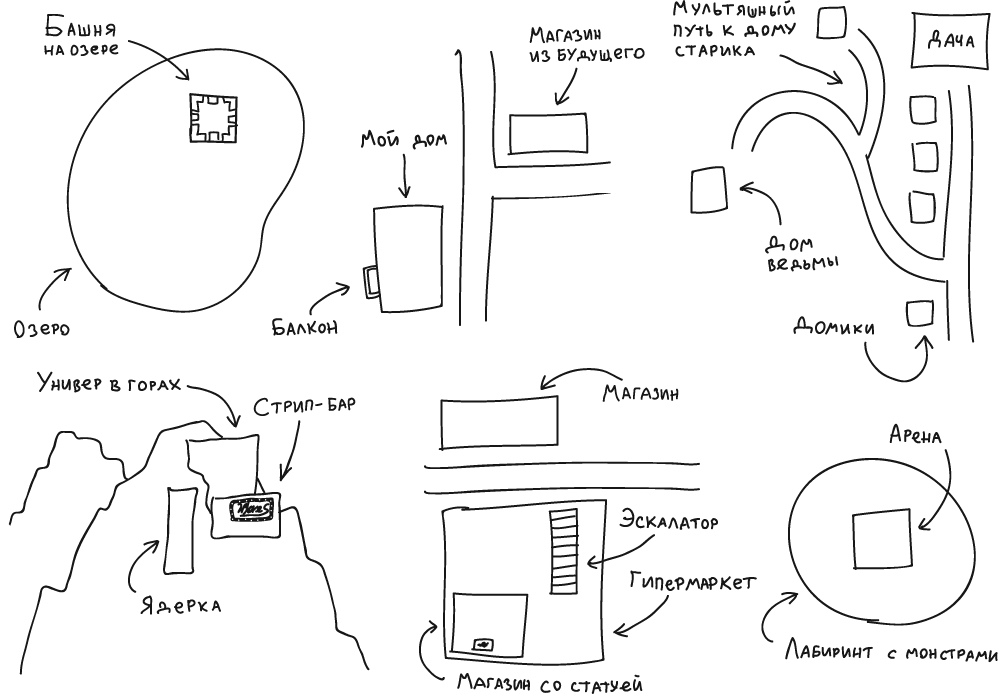
\includegraphics[width=\textwidth]{ris21}
\end{center}
\captionsetup{figurename={Рисунок}}
\caption{}
\label{primer1 }
\end{figure}	

\medskip

\begin{figure}[h!]
\begin{center}
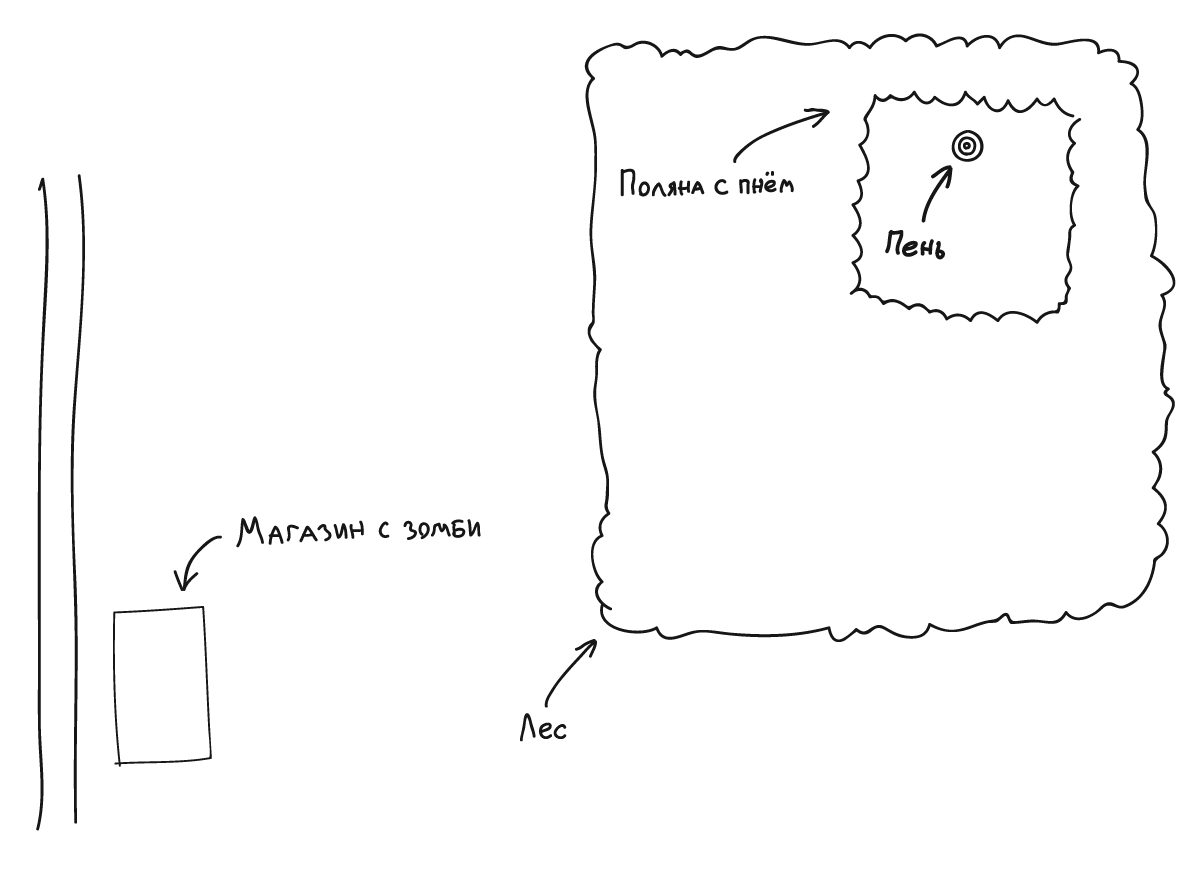
\includegraphics[width=0.9\textwidth]{ris22}
\end{center}
\captionsetup{figurename={Рисунок}}
\caption{}
\label{primer2}
\end{figure}

Сразу поясню, как именно рисовать. В итоге должно выйти что-то вроде Google Maps, то есть схематичное изображение с видом сверху. Отмечать на локациях нужно объекты, с которыми ты взаимодействовал, или которые сильно привлекли твоё внимание.
 
Собственно, рисунок \ref{primer1 }~--- общий. А рисунок \ref{primer2} показывает, как надо зарисовать следующий сон: <<Был в городе, зашёл в магазин, там был продавец зомби, купил у него BFG9000, вышел из магазина, оказался в лесу, там была поляна с пнём, пень я из БФГ взорвал>>. Поначалу локации можно рисовать где угодно на карте, уже потом станет ясно, где и что должно располагаться.


Ещё уточнение: есть у тебя, например, три сна, все три происходят в универе, но в одном универ стоит в горах (на этом зафиксировалось внимание), в другом у него в центре торчит ядерная ракета, а в третьем есть стрип-бар, то локация должна быть одна, то есть универ в горах, из которого торчит ядерная ракета и с зоной стрип-бара (см. первый пример).

Итак\ldots Во-первых, как правило, сразу становится понятно, что ВНЕЗАПНО, из этих 30 снов, половина происходит в 5--6 почти одинаковых местах, но дальше веселее, а именно~--- на определённом этапе у тебя начнут вспыхивать те сны, что ты давно забыл. Выглядит это так: <<Рисует Доброанон эту карту и вдруг ВНЕЗАПНО (прям такое эталонное внезапно) понимает, что этот магазин находиться должен вот тут! А между ним и этим парком был тот сон! А ещё в самом магазине было вот это и вот это, а рядом с ними на том озере было ещё вот то!>>. Как-то так. Ощущения действительно фееричные, целые десятки снов могут вспомниться за одно мгновение.

Конечно, так будет не сразу, <<вспышки>> будут идти постепенно вместе с заполнением карты. Но, если в дневнике уже есть хотя бы 20 снов, то, как правило, даже во время первого заполнения, 3--6 снов вспомнить можно. 

<<Это, конечно, прикольно, но нахуя?>> — спросишь ты меня. Ну, помимо того, что это просто весело, заполнение карты очень сильно улучшает сновидческую память (сны запоминаются идеально), на определённом моменте происходит вспоминание всех снов вообще; кроме того, можно просто бросить взгляд на этот листок, и тут же повалит лавина образов и воспоминаний. Если поутру не можешь вспомнить, что снилось, то также часто помогает пробежаться взглядом по карте. Применений много, пробуй, анон, экспериментируй, думай.

\smallskip

\fancybreak{* * *}

Как это работает? Если в двух словах, то сновидческая память неактивна ввиду редкого обращения к ней. Чем чаще мы к ней обращаемся, тем лучше она работает.

Если более подробно, то картография — это некий аналог фотографии. Ну, например, ездил ты лет этак шесть назад на море, сейчас уже и не помнишь, как оно там было, а вот посмотрел на фотографию~--- и сразу лавина образов, ты за долю секунды вспоминаешь очень много из того отпуска.
 
Это нам и нужно, так как смотря на карту, ты обращаешься к сновидческой памяти, тормошишь её, и чем больше на ней изображено <<фотографий>>, тем больше снов ты вспоминаешь практически одномоментно. По сути, это те же символы, просто скорость чтения у человека ограничена (кроме того, это поначалу снов немного, а когда их Over 900, в дневнике перечитывать их становится сложно), а вот чтобы воспоминания всплыли от созерцания закреплённого за ними символа, времени много не надо. 

Теоретически, в один прекрасный момент при взгляде на карту будет достигнут <<критический>> уровень одномоментного вспоминания снов  (да уже месяца через два, смотря на неё, ты будешь прямо-таки переноситься в мир снов), это, в теории, будет походить на волну, которая окончательно разрушит перегородку между обычной памятью и сновидческой. Больше разделения не будет, и, как следствие, каждую ночь сны будут запоминаться неотличимо от RL, ну и ОСознавать можно будет чаще. Это уже скачок на качественно новый уровень работы с ОСами. Именно к этому и нужно стремиться. 



\chapter{Восприятие осознанных сновидений}


\section{Про осознанность}
Для удобства представим себе палку (лол) с ВНЕЗАПНО двумя концами: один конец~--- это, грубо говоря, обычное наше восприятие IRL, когда мы понимаем, что вокруг происходит, <<Кто все эти люди?>>, где мы и т.д. Бессознательное есть, но оно молчит, и разум находится в <<хватке>> сознания со всеми его таблицами и прочим. Другой конец этой воображаемой палки~--- это наше сновидческое восприятие; бессознательное во все поля, между мыслью и действием практически нет разницы, цепочки взаимосвязанных событий легко заменяют друг друга. Представили, да?
 
Теперь добавим, что на этой палке есть колечко~--- это наша психика в конкретный момент времени. Днём оно находится у одного конца палки, ночью, когда мы спим,~--- у другого. Это, я думаю, тоже понятно. А вот теперь важный момент~--- допустим, мы осознались во сне. Что происходит с колечком в этот момент? Правильно, оно сдвигается чуть чуть в противоположную от конца <<сна>> сторону. Угу? Однако, после этого, когда мы проснулись, оно ВНЕЗАПНО возвращается отнюдь не туда где было раньше, во время бодрствования, а чуть-чуть ближе в сторону сна :3 Этот прикол работает и в обратном направлении.
 
То есть происходит взаимопроникновение плюшек :3 Во снах мы получаем чуть больше осознанности и логики, а днём чуть больше свободы мышления и <<шёпота>> подсознательного. И то, и другое крайне полезно.
 
Это я к тому, что <<Не надо насильно заставлять себя концентрироваться IRL>>, скорее наоборот, нужно расшатать <<тиски>> контроля, например, делая что-то непривычное (стихи читать, ага).
 
Иными словами, тут дело в опыте: как бы начинающий не корячился, в первых ОСах всё равно особо долго он не продержится. Усилием воли удерживать осознанность адово сложно, и уж, конечно, тут о сколь-либо долгих экспериментах речи не идёт. Но со временем ОСы будут становиться стабильнее, потому что идёт взаимопроникновение дневного и ночного режимов работы психики. А что будет когда колечко дойдет до середины? Ну, в теории этот момент я описал в <<картографии>> (опять же, понимаем, насколько она полезна, да?), а на практике\ldots Наверное, тогда человек и становится <<сноходцем>> :3 Надеюсь, мы сами об этом когда-нибудь узнаем, ня :3 



\section{Таблицы восприятия}
В контексте ОСов эта мини-статья, думаю, будет очень к месту. 

Итак, представим себе экселевскую таблицу, вот первая графа: яблоко~--- круглое, растёт на деревьях, вкусное/невкусное, его едят люди, его собирают в корзинах, продают на рынке, оно называется <<яблоко>>, оно может быть зелёным или красным, оно сочное, при желании им можно уебать, ну и ещё намноооого больше 9000 пунктов. 

Вся подобная информация поступает в эту таблицу вместе с ростом человека. Каждого с детства учат, что вот это~--- <<стул>>, на нём сидят. А это~--- <<огонь>>, он может обжечь. 

Соответственно, у каждого в голове формируется такой невьебенный экселевский файл. И когда мы видим нечто круглое и красное, растущее на деревьях, то сознание тут же обращается к этой таблице, ищет соответствия и выдаёт нам, что это <<яблоко>>. 

Основная идея понятна? Отлично, едем дальше. 

Теперь несколько интересных моментов:
\begin{enumerate}
\item Таблица может быть как стабильной, так и не очень, яркий пример~--- это облака\ldots Кто-то видит в них жирафов и слонов, а кто-то просто тучки. 
\item Если человек увидит что-то выходящее за пределы этой таблицы, то тут есть несколько вариантов развития событий:
\begin{itemize}
\item Человек теряет сознание, этакий фатал эррор (Например, утончённая дама, вся жизнь которой прошла на балах и во дворце, вдруг стала свидетелем того, как человек застрелился или натолкнулась на другое кровькишкираспидорасило).
\item Человек не замечает этого объекта, то есть просто его тупо не видит, тут из серии <<Этого не может быть, потому что не может быть>>.
\item Сознание судорожно пытается собрать из известных ему определений образ этой НЁХ (в реале такой вариант бывает крайне редко), отсюда летающие слоны во снах, например.
\end{itemize}
\end{enumerate}

Вот мы и подошли к самому интересному~--- тому, как это всё связано со снами. Дело в том, что во сне:
\begin {itemize}
\item <<Хватка>> таблицы ослабевает. 
\item Нет материальных вещей, есть только символы.
\end{itemize}

Вместе это даёт вздрыжне эффект.
 
Например, во сне вам снится дом. То есть это такой лист, на котором написано <<\textsc{Это дом блеать}>>, но дома-то нет! Ахтунг, алярм, что делать? Из таблицы по частям составляется то, что подходит под определение слова <<дом>>. 

Или, например, символ <<опасность>>. Ну как можно изобразить опасность? У опасности нету тела, блджад, но ведь человек привык всё воспринимать через органы чувств, и снова происходит формирование собирательного образа. 

Или, например, такой символ — <<акт какого-либо действия>>… Обосраться, да? И ведь это тоже надо как-то изобразить. 

Теперь ещё пара интересных моментов:
\begin{itemize}
\item Поскольку таблица во сне пластична, то если долго приглядываться к чему либо, возникают сомнения. Например, смотрим на вилку в ОСе, сознание начинает испытывать попоболь <<А это точно вилка? Может быть, это ложка? Она же рядом в таблице лежит>>, хуяк ~--- и вилка превращается в ложку, потом в нож, потом в поварёшку, а потом вас просто выкидывает, потому что так быть не может. Попробуйте, как будет ОС, взять какую-нибудь вещь и начните её рассматривать. 
\item Я думаю, уже стало понятно, почему трудно трактовать чужие сны: у каждого своя таблица восприятия. Например, символ <<бешеная радость>> каждый представит по-своему, но\ldots И тут на сцену врывается третий пункт:
\item Архетипы: это такие символы, которые все (и русский, и американец, и нигра, и чукча~--- все) воспринимают почти одинаково.
 
Например, круг. Круг~--- это солнце, и если во сне будет символ, связанный с ним, то на данном образе обязательно будет в той или иной форме присутствовать круг. Дядя Юнг на эту тему провёл титаническую работу, найдя почти все общие символы в ВНЕЗАПНО старых алхимических трактатах, ещё и лулзов с этого словил, заставив многих учёных срать кирпичами.
\end{itemize}

Вот как-то так, общее введение, так сказать, в тему <<таблиц восприятия>>. Надеюсь, это будет полезно и вдохновит на дальнейшие исследования, ня :3 



\chapter{Уровни сна}


\section{Общие сведения}
Хочу обратить внимание на то, что деление очень очень условно, это нечто вроде деления людей на сангвиников, холериков и прочее, то есть в чистом виде встречается редко :3 Однако, я думаю, эта простая таблица поможет систематизировать свои ОСы.


\begin{center}
\textbf{1lvl~--- Сон про ОС}
\end{center}

\medskip

Из названия, думаю, сразу многое понятно, то есть тебе снится сон, в сюжете которого ты кагбе осознаёшься; тут один из <<детекторов>>~--- это непонимание того, кто ты есть на самом деле, то есть мысли могут быть такими: <<Ух ты, я осознался, а я кто? Ах, ну да, я внебрачный сын Дарта Вейдера, вот папа обрадуется, когда ему расскажу>> и т.\,п.
В принципе, если такой сон был, то это уже хороший признак, он показывает, что ты в одном шаге от полноценного ОСа. То есть, ты действительно этой темой интересуешься и что-то делаешь, но самое главное, что ты ей <<загорелся>>, без этого успехов тут не будет, как и в любой другой области, связанной с психикой.

\bigskip

\begin{center}
\textbf{2lvl~--- Просто ОС}
\end{center}



Обычно бывает так: во время сюжета посещает мысль <<Сплю ли я?>>, после чего  (если, конечно, делал <<руку>>) смотришь на свою ладонь и~--- БДЫЩЬ, ОСОЗНАННОСТЬ. Первый раз длится недолго, конечно, но ты уже чётко понимаешь, что это сон, а главное~--- понимаешь, кто ты есть в реале. Как правило, заканчивается это счастье провалом в сюжет, можно потом, анализируя сон, заметить момент перехода, например: <<Я вошёл в класс, осмотрелся и решил подойти к преподу-инопланетянину, но (внимание) решил, что нельзя его беспокоить посреди лекции>>~--- вот это уже попадание в сюжет, человек забыл, что это сон.

По яркости бывает по-разному, но особо ярких впечатлений, как правило, не оставляет.

\textit{(Обратите внимание, что главное различие между первым уровнем и всеми остальными состоит в том, что в действительно осознанном сне, сноходец более-менее четко помнит кто он, какое сегодня число, где он сейчас спит и так далее --- примечание редактора)}



\begin{center}
\textbf{3lvl~--- Глубокий ОС}
\end{center}



От прошлого отличается так же, как 1lvl от 2lvl :3 Вхождение происходит или через руку, или через некоторые трюки во сне (как правило, неосознанные), оставляет ОЧЕНЬ яркие впечатления, кажется, что всё намного ярче и живее чем IRL, море впечатлений, в общем.

Заканчивается или погружением в сюжет, или пробуждением.



\begin{center}
\textbf{4lvl~--- Сверхглубокий ОС (<<Фаза>> по терминологии Михаила Радуги)}
\end{center}


Вот это отдельная песня, бывает он в двух случаях, рассмотрим их отдельно.
\begin{enumerate}
\item Случайный выход. Происходит он примерно так: просыпаешься ты в один прекрасный день, идёшь в туалет, чистишь зубы, закуриваешь сигарету и садишься за чтение твоего любимого Доброчана :3 В особо тяжёлых случаях можешь даже сходить в магазин за пивом\ldots и только потом обнаружить, что ЭТО СОН БЛЕАТЬ!!11. Например, придя домой из магазина, ты замечаешь, что диван поменял свой цвет. При этом точно понимаешь, кто ты, что делал IRL вчера, никаких летающих бегемотов на улице нет, и вообще от реальности отличий очень мало. Хотя сюжет иногда возможен, например, ты уверен, что у тебя живёт друг или тян :3, или твоя квартира находиться в другом месте, но при этом всё очень достоверно.

Спонтанно такое бывает редко (но метко, отсюда мноооогие истории про астралы и т.д.), и, если уж случилось, то можно очень нихуёво просраться кирпичами. Но пугаться не нужно, рука работает и тут, так как любое напряжение (эмоциональное или какое ещё) заставляет даже этот уровень ОСа меняться и <<течь>>. Я для себя, например, выработал такую практику: два раза в день (утром и вечером) я громко и с выражением читаю небольшие стишки. Это, конечно, уже паранойя, но раза три я так ВНЕЗАПНО обнаруживал что оказывается это сон\ldots хотя на первый порах об этом париться не надо, вот как случится~--- тогда уже можно :3
\item Намеренный выход. Тут лучше всего воспользоваться <<не\-пря\-мы\-ми>> техниками Радуги, и да, многие, кто долбились во всякие астралы, ВТО и прочее, насилуя себя попытками днём вывалиться <<из тела в вихре>> занимались на самом деле <<прямыми>> техниками попадания на 4lvl ОСа. Прямые техники я категорически не рекомендую делать ранее, чем через месяц после занятий по <<непрямым>>. Также возможно попасть в этот левел и через промежуточное состояние (<<дрёму>>), но это~--- отдельная тема.
\end{enumerate} 
 
Как выходить намеренно, что вас там будет ждать, советы как там удержаться~--- всё это чудесно написано у Радуги, я вот честно лучше него написать не смогу. Читайте, я рекомендовал мало книжек, но все они очень-очень дельные.

\clearpage

\begin{center}
\textbf{5lvl — ВНЕЗАПНО реальный мир :3}
\end{center}


Шутка :3 Хотя, как известно, в каждой шутке\ldots
\medskip

И ещё, важно уяснить одну вещь: деление условное, кроме того, при желании можно и со второго  уровня <<залезть>> на четвёртый, про <<углубление>> написано у Радуги. Это я к тому, что не не надо <<ждать у моря погоды>>, мол <<У меня был второй левел, подожду, когда будет третий>>, нужно пробовать углублять то, что получается, всё в твоих руках/мозгах, анон :3



\section{Понятия ОС и фазы}

\begin{tikzpicture}
\node [fill=futababack,rounded corners=5pt,text width=13cm]
{
Кстати, правильно ли я понял, что ОС~--- это неглубокая фаза, в которой надо пытаться углубляться? Или это одно и тоже?
};
\end{tikzpicture}

Ладно, няши, позвольте мне попробовать устранить путаницу в терминах и понятиях, заодно пояснив, откуда она взялась. Думаю, всем полезно будет. 

Сначала разберём термин <<фаза>> и выясним, откуда он взялся и что означает.

В этом треде термин <<фаза>> появился из литературы за авторством некоего Михаила Радуги; оный Радуга, с его слов, и ввёл сей термин. Внимательно прослушав вступление к семинару, можно легко понять, почему и зачем он это сделал. Дело в том, что сей шкафообразный господин пытается усидеть на двух стульях (что при его габаритах неудивительно), а именно~--- сплотить вокруг себя как материалистов, так и эзотериков (что косвенно подтверждается резким контрастом между названиями его книг и их содержанием), считая природу астрала/ВТО и осознанных сновидений одинаковой. Он не мог назвать сие замечательное явление астралом, так как FUUU-эффект с материалистической части аудитории был столь же предсказуем, сколь и неизбежен; осознанным сном Михаил это дело называть также не стал, справедливо остарегаясь эзотерического бунта (какому же эзотерику понравится, что его бесценный внетелесный опыт обзовут всего лишь сном, пусть и осознанным?). Именно по этой причине (типа, чтобы никому не было обидно) Радуга ввёл термин <<фаза>>, обозначив им весь широчайший спектр явлений, среди которых находятся и осознанные сновидения в понимании Лабержа, и всё многообразие внетелесных ощущений в эзотерическом смысле. Глубокий астрал, неулубленное состояние через осознание во сне~--- явления одного порядка с точки зрения Радуги, и всё это~--- фаза. У него есть градации глубины погружения, но на уровни он фазу не делит.

Разобравшись с происхождением, двинемся дальше и изучим, как изменился смысл термина, попав в тред. Так исторически сложилось, что практическим пособием в треде считается как раз литература Радуги. Многолетняя практика позволила ему выделить три способа попадания в фазу (которая ОС и она же астрал).

Первый способ~--- это традиционное для материалистов осознание из сна, достигаемое путём направленного желания, тренировки сновидческой памяти и развития критичности восприятия. Обычно, если неподготовленный человек понимает, что спит, то он тут же просыпается. Подготовка направлена как на увеличение частоты осознаний, так и на способность не просыпаться, а оставаться во сне, получая контроль над его сюжетом. Радуга очень мало говорит об этом способе входа в фазу, считая его крайне неэффективным.

Второй способ~--- столь же традиционный, но уже эзотерический: вход прямыми техниками. Если материалисты стараются достигнуть состояния <<тело спит, мозг бодрствует>> методом <<сначала усыпить тело и мозг, а потом аккуратно разбудить мозг>>, то эзотерики подходят к той же задаче с другой стороны: пытаются усыпить/отключить тело, оставив мозг бодрствующим. Суть метода~--- использование фантомных ощущений любого характера для достижения состояния плавающего сознания, а затем резкого переключения с реальных ощущений на фантомные (так называемое <<разделение>>). Этот метод Радуга также настоятельно не рекомендует, так как считает его невероятно сложным для новичков и по этой причине губительно сказывающимся на мотивации практикующих.

Ну и наконец, третий способ, который Радуга рекомендует как наиболее доступный широким слоям населения~--- вход непрямыми техниками, которые Радуга, вроде как, изобрёл. Основное отличие от прямых заключается в том, что прямые техники делаются обычно вечером, на фоне засыпания, а непрямые, наоборот, утром, сразу после пробуждения. Идея метода основана на том, что достигнуть состояния плавающего сознания вечером, когда мозг толком не хочет спать, намного сложнее, чем утром, когда он не успел как следует проснуться. Мой личный опыт подтверждает, что вызвать фантомные ощущения непосредственно после пробуждения намного легче, чем вечером, и они получаются гораздо убедительнее.

Так как в книгах Михаил почти не говорит об осознании из сна, а Лаберж почти не говорит о прямых (а тем более~--- непрямых), и при этом они оперируют разными терминами, в голове у читателей непроизвольно формируется впечатление, что речь идёт о разных вещах~--- ОС достигается осознанием из сна, а фаза~--- прямыми и непрямыми техниками. Оное впечатление усиливается, так как Радуга много пишет и говорит об углублении и только углубленную фазу считает полноценной и клёвой. Но на самом деле, согласно Радуге, способ входа почти не имеет значения~--- и при осознании из сна, и при входе прямыми/непрямыми мы получаем примерно одно и то же состояние, и оно тут же требует углубления. 

Также есть мнение, что фаза, достигнутая прямыми/непрямыми техниками, сама по себе является глубокой, и дальше углублять и стабилизировать её не нужно. Так бывает, но абсолютно не всегда. Кашу не испортишь маслом, а фазу~--- углублением, независимо от способа её достижения.

Теперь про уровни. Типичной ошибкой является мнение, что уровень~--- это нечто конкретно-незыблемое и постоянное (как минимум, в пределах одного сна). Это не так, разумеется; даже само существование техник углубления и стабилизации это показывает. Осознался среди розовых летающих крокодилов (вроде как второй уровень), потом углубился, да так, что взлететь не можешь, побродил, потом увлёкся чем-либо и скатился обратно, а то и ещё дальше~--- провалился в обычный сон\ldots Какой это был уровень? Вот так и не скажешь, так как и сами уровни условны, и состояние меняется. По своей практике могу заметить, что более <<мелкие>> фазы характеризуются расплывчатостью и заторможенностью мышления, низкой (относительно) реалистичностью окружающей действительности, присутствием во сне нелогичностей~--- как вокруг, так и в собственных поступках (например, встретил друга, начал ему рассказывать и доказывать, что это сон. А зачем? С какой целью? Ещё пример от Радуги: открыл холодильник с целью пожрать чего-нибудь, а оттуда как посыпятся сырки глазированные, ну он давай их собирать. Опять же, зачем? Подобные действия как раз свидетельствуют о неглубокой фазе), но зато окружение более пластично, податливо. Можно взлететь и полетать, можно пройти сквозь стену, можно даже сотворить из ничего тян. В глубоких же фазах (обычно достигаемых при помощи углубления и удерживаемых техниками стабилизации) окружение сильно напоминает RL, в том числе и по стабильности~--- фаербол не кинешь, крылья не отрастишь. Точнее, можно, конечно, но, по-моему, не для новичка. Я бы назвал такие приёмы техниками локальной дестабилизации, но диванные теоретики настолько диванны, что не могут в фазе проверять свои теории. Поэтому пока как-то так.




\section{Подробнее о механизме 4 lvl/фазы!}  
Это всё, действительно, очень похоже на <<выход души из тела>>, но попробую объяснить, как я это вижу с научной точки зрения.

Итак\ldots Многим в детстве снилось, что они начинали падать, и просыпались от столкновения с землёй, обычно ещё было ощущение как будто бы реально упал, на самом деле дёргалось тело, так как мозг начинал его пинговать на предмет <<ты ещё там живо?>>. К слову, я уверен, что так же некоторые из вас испытывали перед засыпанием <<толчки>>, то есть нога или рука <<случайно>> сама дёргается, выбрасывая вас из дрёмы. Мистики тут нет, просто организм начинает очень глубоко засыпать. Чтобы сон не стал <<бесконечным>>, существуют некие структуры, которые регулируют глубину сна, если разуму кажется, что сон стал уж совсем глубоким, то он посылает тот самый <<пинг>>.

Во многих <<прямых>> практиках есть момент с <<вызыванием ощущения падения>>, что, по сути, бывает при (барабанная дробь) потере сознания. А вот щас, внимание, прочувствуйте эту фразу~--- <<потеря сознания>>. Я знаю, у многих возникла стереотипная реакция типа <<когда человек падает>>, но я хочу, чтобы вы вдумались в смысл фразы <<потеря сознания>>. Вдумались? Хорошо.

Едем дальше~--- <<наблюдение вспышек и образов перед глазами>>, ВНЕЗАПНО характерно для той же потери сознания. Раскачивание фантомного тела~--- <<Я вроде как чувствую, что стою, но тело падает>>~--- это из анамнеза одного человека, болезнь которого так же не менее ВНЕЗАПНО имеет симптомы потери сознания. Мысль уловили? Получается, если 2--3 lvl ОСа это <<осознанный сон>>, то 4  уровень это <<осознанная потеря сознания>>, лол :3 

Как мне видится это процесс? 

Возьмём, для примера, непрямые <<утренние техники>>. Человек проснулся, он ещё не пришёл, грубо говоря, в то самое <<сознание>> и начинает <<раскачивать>> фантомное тело. То есть в мозг поступают псевдо-сигналы, что происходит движение. Мозг негодует! Как это так!? Тело же лежит, блджад! Однако фантомные движения становятся всё более отчётливыми, псевдо-тело готово встать, и тут перед разумом встаёт дилемма: он должен <<выбрать>>, в каком <<теле>> оставить точку сознания.
 
Если в физическом, то человек просто теряет сознание, что потом переходит в сон, а если в  <<фантомном>>, то сознание переключается на работу <<вовнутрь>>. Дабы не было фатал эррора, начинается постройка окружающего, исходя из основных моментов памяти человека и его таблицы восприятия, потому что вариантов больше нет. То есть разум (обобщённое слово, но тут оно больше подходит) начинает строить мир в голове, так как <<тело вроде как движется именно там>>.

Вот, собственно, и всё :3 Понимаю, что теория хлипкая, но других я пока не слышал, если у кого-то есть лучше в научной модели, то просьба поделиться.




\chapter{Персонажи сна}

\section{<<Мы>> во сне}
Ну, вернёмся ко снам. Перво-наперво надо ещё раз вспомнить, что во сне физических объектов нет. Об этом многие постоянно забывают, и это сильно тормозит дальнейшие успехи в ОСах. 

Всё, что мы там <<видим>>~--- это символы, которые наше сознание интерпретирует на основе своей таблицы восприятия. Это раз. 

Два~--- это понятие времени. Я считаю, что и IRL это штука субъективная, а уж во сне и подавно. Можно представить себе сон таким образом: сознание единовременно получает пакет зашифрованной информации и начинает люто, бешено её декодировать, переводя в понятные для себя образы/звуки/запахи/чувства и т.д. 

Что из всего этого следует? А то, что <<мы>> во сне~--- вовсе не личность и не то, что там бегает, и даже не то, от чьего лица мы это наблюдаем. Мы там~--- это просто точка наблюдения. А всё остальное~--- тот самый блок информации. 

То есть весь сон, включая даже тех <<нас>>, <<наши>> ощущения, и прочее~--- это просто одно большое кино. % Для соснолеёба кинцо везде, лолка
  
Очень долго думал над аналогией, дико обрадовался когда нашёл, так вот: вспомним, что происходит, когда мы читаем книгу. Вот если по факту взять: человек пырится на куски бумаги, с нанесёнными на них чёрточками, при этом он переживает, испытывает эмоции, зачастую даже почти что галлюцинирует. Удивительно, да? Казалось бы~--- RL, сознание на месте, и тем не менее человека не шокирует, что, смотря в листы с чернилами, у него в голове разворачивается целая история.
 
Просто сознание поглощено анализом и переработкой поступающей информации.
 
По большому счёту, разницы между чтением книги и сном нету. Просто с книгой информация поступает только зрительная, а во сне она идёт по всем каналам. Это естественный механизм восприятия, иногда ещё говорят, что человек поглощён <<фильмом, книгой, игрой, работой, мыслью>>. Чтобы в полной мере, насколько это возможно, осознать поступающую инфу, которая у него под носом, происходит частичное абстрагирование от окружающей действительности. Это, увы, обусловлено ограничениями нашего сознания, так как одновременно, например, читать, писать и говорить человек не может, хотя вроде были прецеденты. 




\section{NPC}
Перво-наперво нужно понять, что во сне нет тела, рук, ног, глаз, языка и всего прочего. <<Видим и слышим>> мы там исключительно потому, что привыкли воспринимать мир подобным образом. Во сне это часто играет с нами злую шутку, так как если мы там видим (и, что немаловажно,~--- слышим) символ или какую-либо информацию, не встречающуюся в чистом виде IRL, то для её восприятия собирается звук или изображение, исходя из того, что мы знаем. Отсюда летающие бегемоты и бредовые диалоги с NPC. 

Но тут есть интересный момент: некоторые NPC общаются во сне <<пониманием>>, ещё можно сказать <<телепатией>>, то есть слов нет, но ответ ты ВНЕЗАПНО понял очень чётко (это будет подробнее рассмотрено далее). В чём же отличие между <<говорливыми>> и <<телепатическими>> NPC?

Вот мы и подобрались к самому интересному. Надеюсь, что Юнга большинство уже прочитало, ну, в любом случае, слово <<Архетипы>> слышали все, наверное. Это первоосновы нашей психики, сидящие в таких её глубоких ебенях, что и подумать страшно. Они были у нас с рождения и связаны, насколько мне представляется, с генетической памятью. В общем, вся наша невьебенно глубокая личность и Очень Богатый Внутренний Мир по сравнению с ними~--- просто наносной пшик.
 
\begin{figure}[h!]
\begin{center}
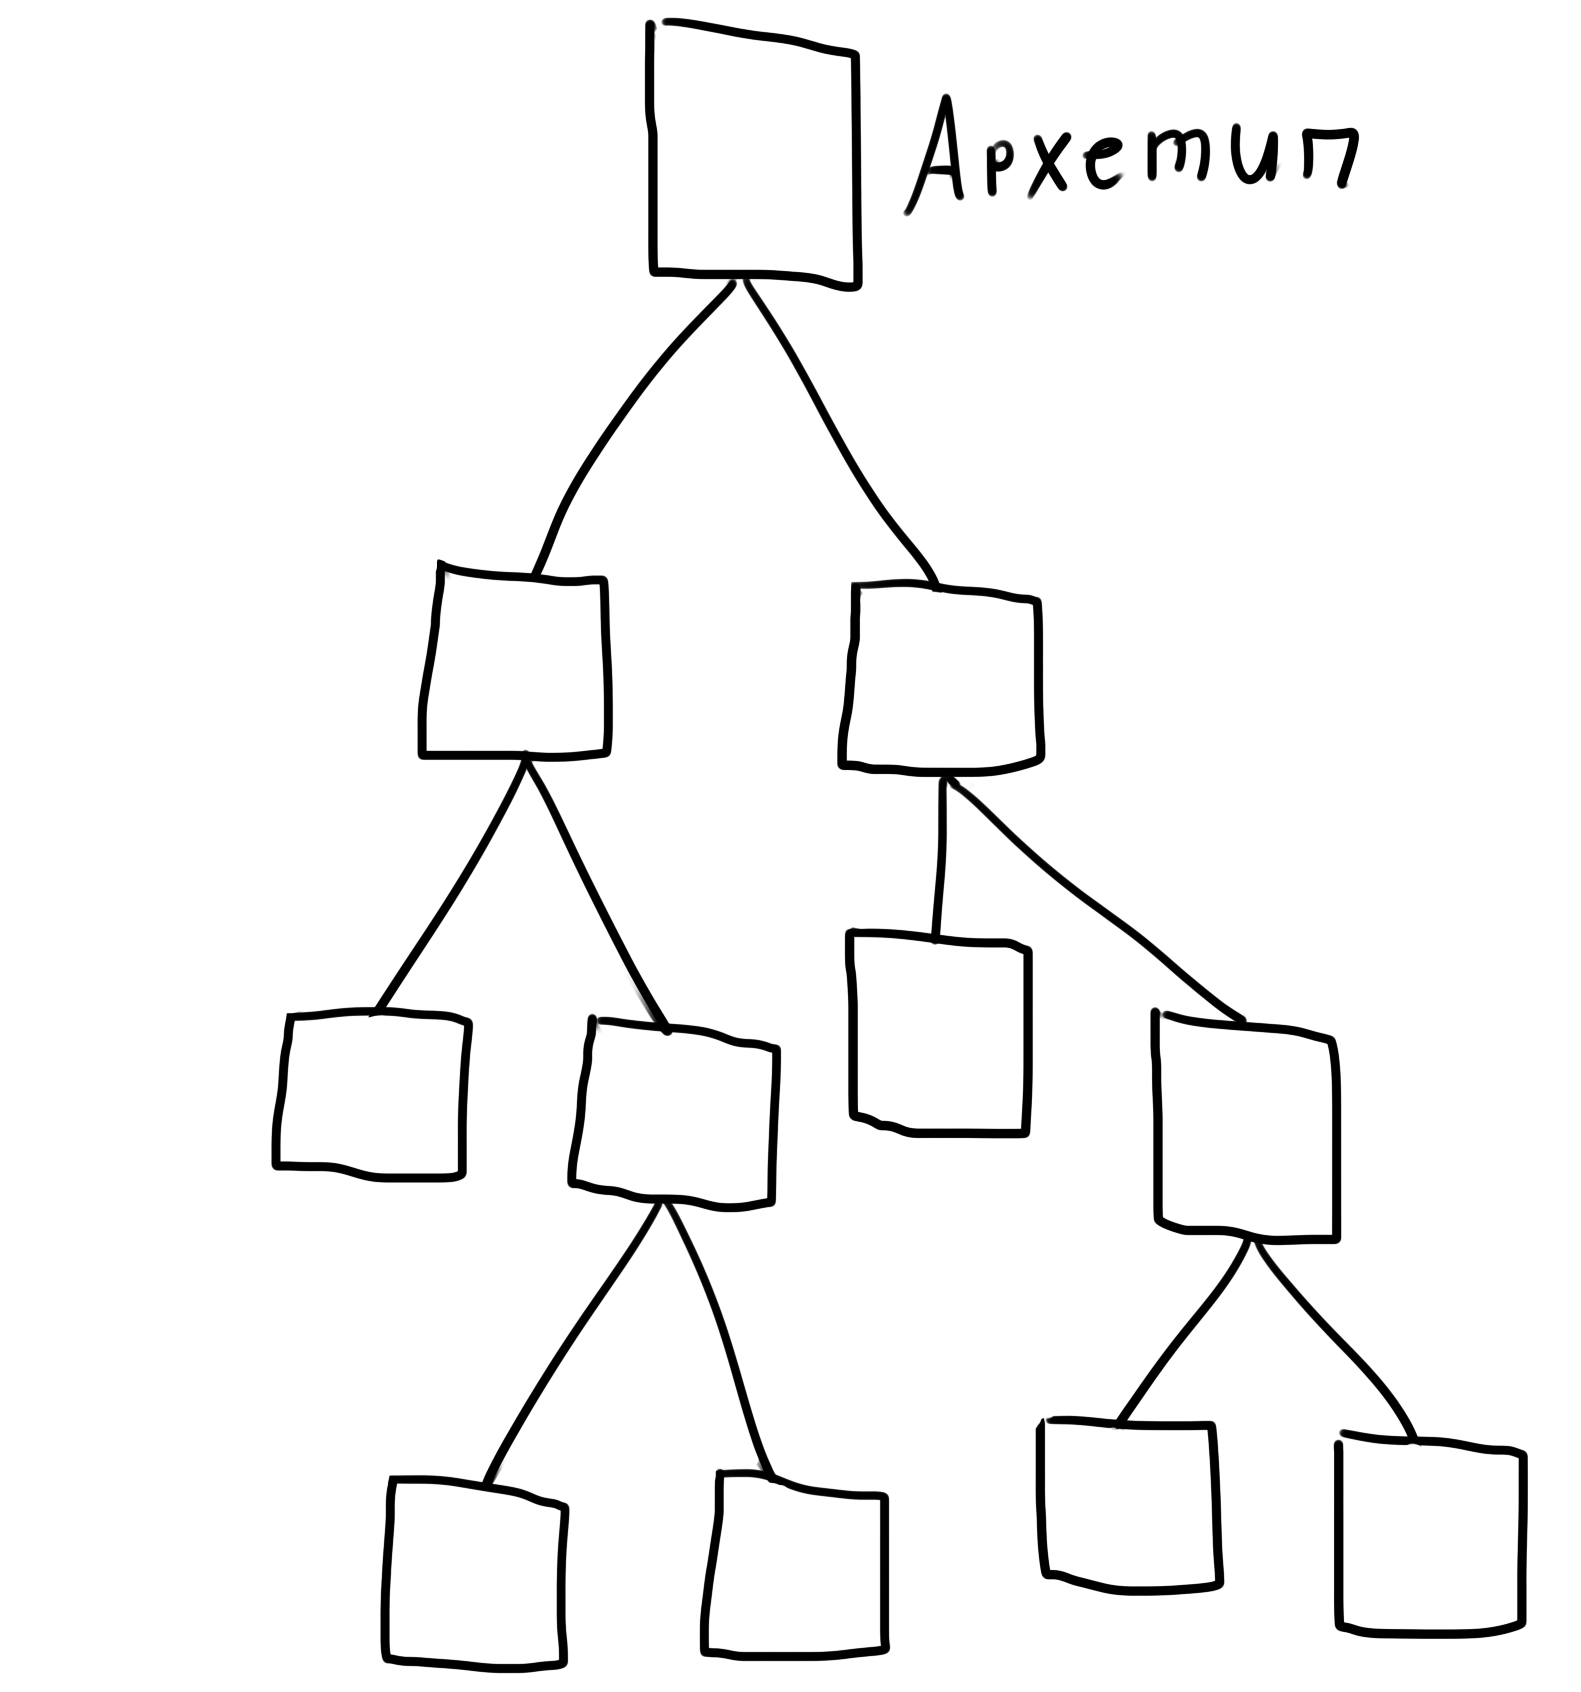
\includegraphics[width=0.9\textwidth]{ris81.png}
\end{center}
\captionsetup{figurename={Рисунок}}
\caption{}
\label{archt}
\end{figure}

Теперь смотрим на рисунок \ref{archt}. Архетип~--- это основа, так сказать, ключевой элемент конструктора, из которого во сне собирается ВСЁ, с чем мы сталкиваемся. Рисунок, конечно, утрирован, так как на самом деле конструкции гораздо более многоуровневые. Итак, можно сделать вывод, что есть NPC, которые <<ближе>> к изначальному Архетипу, точнее, к группе Архетипов, хотя бывает по-разному, а есть <<далёкие>> его бледные отражения.

Что же нам полезного даёт весь маразм, написанный выше?

А даёт он нам главный вывод~--- чем ближе NPC к <<истокам>>, тем лучше, понятнее и информативнее он с нами общается. Отличить их достаточно просто~--- часто сам начинает разговор; стабилен; может переходить за сновидцем по локациям, а иногда и по снам, иногда даже по разным, например, целую неделю шататься рядом, если ему что-то очень <<хочется сказать>>; общается <<пониманием>> или связной и понятной речью; вызывает некий внутренний <<трепет>>; чихать он хотел на ваши приказы и попытки как-то его изменить и т.д. :3 Ну вот, навскидку всё.

С такими NPC общаться можно и нужно, тем более что они, как правило, первыми начинают разговор. 

Иногда <<глубоких>> можно встретить просто во сне, обычно впечатления остаются на всю жизнь. Я вот, кстати, после пары таких встреч начал прекрасно понимать всяких жрецов древности, к которым во сне <<приходили Боги>>: после таких снов, не зная о психологии, можно запросто ебануться на отличненько и решить, что к тебе кто-то являлся. Уж больно феерические ощущения.

Подробнее архетипы разобраны в следующем разделе.

Ну вот такое маленькое введение в мир сновидческих NPC :3 

Теперь практика для тех, кто имеет хотя бы три ОСа в неделю.

Значит так, стена выше, надеюсь, вызовет резонный вопрос: <<А если я хочу целенаправленно найти глубокого NPC, то как это сделать?>>. Ответ простой: во сне всё очень буквально, и если мы ищем тех, кто символизирует глубины нашей психики, то нужно идти <<вглубь>> :3 Да-да, это пещера или, например, спуск в катакомбы. Как правило, там есть дверь/река/стена и т.д., через которую нужно перебраться. Кроме того, во время спуска становится очень сложно удерживать осознание, так что надо подготовиться. Ну и кроме возможности встретить там вздрыжне персонажей, на <<глубине>> можно проводить более серьёзное и продуктивное изменение/лечение своих багов, да и вообще отлично покопаться в своей голове. 

\begin{shaded}

\begin{center}
\Large\textbf{Кулстори: уберпамять}
\end{center}


А, да, когда-то обещал кулстори для мотивации людей на занятия ОСами, собственно, вот.

В одном из экспериментов (тред восьмой или девятый, если хотите найти) решили попробовать воздействовать на память. Идея была такова: найти реку Мнемосины (Др. Греция, мать всех муз, если не туплю), испить из неё. В следующем ОС я нашёл эту речку; что забавно, это одна из двух рек, что у меня в мирке есть. Когда я выпил воды, ещё в ОСе на меня нахлынула волна образов из памяти. Я попробовал сконцентрироваться на определенном событии, результат~--- конкретное воспоминание об этом событии.

Чем черт не шутит, попробовал воспроизвести ощущение на экзамене, <<списать>> с памяти конспект. Не поверите, но вышло. Если сам ещё вывел один вопрос, то второй я списал ровно по памяти из конспекта. Сдал на 4 (я распиздяйничал весь семестр :3).

Для ещё большей мотивации имею ещё один опус:

В общем-то доупарывался я с ОСовым взаимодействием до такой степени, что дошёл до архетипичных образов. Собственно, есть у меня Мудрец как персонаж, говорит часто, помогает с выполнением некоторых дел советами и так далее. Однажды навёл порядок у него в локации (библиотека), после этого он сказал, что может быть со мной постоянно и давать советы. Как оказалось, я научился (он научил?) устанавливать с ним контролируемый внутренний диалог, чем пару раз пользовался даже для входа в ОСы. Вот такие дела, можете меня считать шизиком :3

\end{shaded}

\section{Общение с NPC}

\begin{tikzpicture}
\node [fill=futababack,rounded corners=5pt,text width=13cm]
{
Просто именно осознанно я не пробовал общаться на уровне понимания. Вот сейчас я все понял только с утра. И ведь действительно как понимание: это был не логический вывод из ОСа, а уровень ощущений.
};
\end{tikzpicture}

\medskip

Лол'д, а как же ты там общаешься? :3 У тебя нет во сне тела, нет рта и нет языка :3 Просто ты привык, что при общении твои <<посылы>> обретают форму слов. Как, собственно, и обратное направление: если кто-то тебе что-то сообщает, то ты это слышишь. Но вот беда: если со зрением во сне бывают глюки в виде <<бегемотов с реактивным задом>> (вспоминаем таблицу восприятия), то со словами ВНЕЗАПНО происходит то же самое, и если персонаж <<слабый>> и пытается донести до тебя нечто сложное, то в итоге ты получаешь <<словесный бред>>, понятно? :3 

\begin{tikzpicture}
\node [fill=futababack,rounded corners=5pt,text width=13cm]
{
Наловил кучу лулзов из общения с NPC. Вернее они с меня наловили, исходя из того как я пытался их разговорить на интересующие меня темы. Один из них настолько умело мне отвечал (этого человека я знаю IRL), причем совершенно непонятно (вроде и есть смысл в его словах и еще какой! блеать а вроде и полная туфта), что я даже очконул что все происходит на самом деле. Первая мысль у меня была <<Это я же сейчас так жестко затупил, называя реального человека NPC и требуя дать мне ответы на мои вопросы, что просто ёбаный стыд!!>>. Хотя тут же понял, что несет он по большей всякую ахинею и этого не может быть.
};
\end{tikzpicture}

\medskip

Ну, я же писал, что с простыми NPC общаться не очень :3 Ищи тех, кто общается с помощью <<понимания>>; кстати, если уже ОСы более-менее частые, то пробуй, как я писал, пробираться <<вглубь>> локаций, во всякие подземелья и подвалы, там шанс найти более <<глубокий>> (игра слов, да, но в нашем случае она ВНЕЗАПНО очень логична) символ. А слова и бред с ними~--- это из серии <<летающие бегемоты с шеей жирафа>>, то есть смысл собирается из твоей таблицы. Для сознания он звучит как бред, да.
 
Ну, например, словосочетание <<тёплый цвет>>. Как цвет может быть <<тёплым>>, блджад? Но ведь это имеет свой эмоциональный отклик.
 
Поэтому, например, ответ на вопрос <<А любит ли меня девушка?>> вида <<Птицы, летающие над фонарями, тебе скажут>> может трактоваться так: в детстве ты видел птичек, пролетевших над фонарями на улице, это тебя удивило и вызвало очень приятные эмоции. Соответственно, ответ значит, что <<скорее да, чем нет>>. 

Опять же, подсознание не оперирует логикой, это ты его так воспринимаешь :3 Попытки перевести дико насыщенные ответы, слова, значения которых ты не знаешь, выливаются в тот самый словесный понос, лол :3 

То есть, ещё раз. Например, тебе поступает информация <<Тёплое, мягкое, но в тоже время серьёзное согласие, с некоторыми нюансами, игривостью и намёком на твою лень>>. 
И это всё, сцуко, одним посылом. Соответственно, чтобы воспринять это через <<слух>>, происходит подбор по таблице максимально подходящих образов. Отсюда может родиться, например, <<Котята, думаю, согласны>> :3

\medskip

\begin{tikzpicture}
\node [fill=futababack,rounded corners=5pt,text width=13cm]
{
А классно, ты так задаешь вопросы и получаешь ответы. Это просто <<вопросы>>, или ты как бы внутреннее еще стараешься <<услышать>> ответ?
};
\end{tikzpicture}

Просто вопросы задаю, важно их правильно задавать, но это штука индивидуальная. 

А ответы бывают двух видов~--- на словах, и <<пониманием>> (например, так Юки-куну Анима сказала, что его <<ждала>>). Пониманием общаются очень <<глубокие>> символы, вот как раз те основы, о которых рассуждал Юки, например, вообще словами не говорят. Анима говорит и так, и так, в общем, если что-то общается такой <<телепатией>>, то это что-то серьёзное.
 
Я, например, один раз общался с символом <<явления>>, именно это слово просто у меня ассоциируется с ним; это был вообще майндфак. Ну вот, например, есть поле, тучки, вдруг пошёл дождь. Так вот, то, что он пошёл~--- это и есть <<явление>>. Или по дороге проехала машина, вот то, что она проехала~--- это тоже явление. Сложно, да? Словами в полном объёме не передать, а во сне спросив <<кто ты?>> я сразу получил ответ и всё понял :3

Ну и стабильность NPC: если что-то следует за тобой в ОСе, не меняется и более-менее связно говорит, то это уже повод обратить на него своё внимание. 

\medskip

\begin{tikzpicture}
\node [fill=futababack,rounded corners=5pt,text width=13cm]
{
Сегодня осознался, но быстро провалился в сюжет. Ходил по каким-то подвалам, это был дом демонов, вдруг вспомнил, что это сон, посмотрел на руку, ня. Опять пошёл искать одного куна, как тут говорили~--- звал, надеялся, что он окажется за поворотом <\ldots>
};
\end{tikzpicture}

\medskip
Ну тут это надо не вслух делать, точнее не только вслух. На\-при\-мер, если хотим вызвать аниму/анимуса, то вспоминаем старые сны; как минимум, пару раз в жизни, он/она снились каждому, и это оставляет очень мощные впечатления, которые являются ключом. То есть в ОСе не просто подходим к двери и орём <<Анима, блеадь!>>, а стараемся <<вспомнить>> ощущения от неё в прошлых снах, это уже само по себе действие, то есть нужно помнить, что в ОСе, по большому счёту, разницы между <<подумал>> и <<сделал>> нету. Просто вспоминая о чём-то, ты уже материализуешь это, ну, правда, <<по привычке>> не сразу, а например за дверью, да. 

Кроме того, любое намерение~--- это уже команда, то есть пожелал найти Аниму, а за дверью пусто. Думаешь ну всё, пиздец, проваливаешься в сон, а потом сталкиваешься по сюжету с какой то НЁХ. Да-да, прямо твой пример. Так, собственно, вот это~--- грубо говоря то, почему ты <<Аниму>> не нашёл. Поясню: любая мысль/намерение в ОСе <<материализуется>> моментально, если этого не произошло, то значит, тебя что-то удерживает, что-то мешает, и как только осознанность пропадает, тебе, грубо говоря, показывают репорт, мол <<Дорогой юзер, вот почему был фейл>>. 

На самом деле заморачиваться этим особо не стоит, с использованием <<ключей>> такая хуита обходится на раз. Я это так рассказал, для общего сведения :3




\chapter{Локации сна}

Итак, почему во снах часто фигурируют реальные места, со странными свойствами, и <<народонаселением>>? Причём, зачастую свой <<сновидческий>> функционал они сохраняют из сна в сон.

Давайте сразу возьмём пример. Одна из самых часто встречающихся локаций обладает следующими <<ключами>>~--- присутствует некоторый страх, точнее, даже не страх, а неуверенность и осторожность, с другой стороны, вглубь этого места тянет, хочется его исследовать, если немного подумать, то окажется, что хочется в нём что-то найти. Как правило, место достаточно мрачное, зачастую тёмное, но обладает удивительной привлекательностью. Во сне ты бредёшь по нему, не совсем понимая, куда и зачем, но тебе нравится в нём находиться, тебе интересно, что там дальше. Несмотря на то, что зачастую присутствует ощущение <<взгляда>>, уходить оттуда не хочется. 

Ну как? Вспомнилось что-то похожее? :3 

Скорее всего, это лес, остовы зданий, пустые дома или подземные коридоры. Эта локация называется <<Лабиринт>>, и представляет из себя отражение <<хранилища>> наших подсознательных стремлений, которые зачастую были забыты и заброшены в дальний угол. 

Ещё пример: ты бежишь, зачастую опаздываешь, волнуешься, что-то сделал не так, что-то забыл или не успел. Часто в последний момент обнаруживаешь, что чего-то не хватает, и это тебя гнетёт. С другой стороны, есть предвкушение чего-то нового, того, что оставит позади старое и пройденное.

Это место обычно предстаёт в виде поездов, общественного транспорта, самолётов, метро и прочего подобного. 

Это локация <<перехода>>. Она показывает изменения в тебе, намекает, что ты <<боишься что-то отбросить>>, или что тебе мешает <<частое возвращение к прошлому>>, но, главное, она символизирует, что твоя личность быстро меняется. Это не плохо или хорошо, это факт. Например, такое случается под воздействием настолько большого количества новых знаний, что подсознание решило запилить об этом <<репорт>> :3
   
Теперь разберём, по какому принципу строится <<подборка>> таких локаций.
 
Как я уже говорил, при попытке понять, как работает подсознание надо мыслить буквально. Не нужно мудрить или искать скрытые подьёбы. Подсознание этого делать не умеет, оно просто показывает важную информацию, а ты в свою очередь воспринимаешь её на основе своего опыта. Можно сказать по-другому, не совсем правильно с технической точки зрения, но легче для того, чтобы уловить суть: ты в процессе жизни учишь подсознание, как показывать ту или иную информацию.
   
Приведу такую аналогию. Вот у нас есть компьютерная игра с персонажами, строениями и прочим. Допустим, что она стоит на двух разных компьютерах. Данные о том, что <<вот тут должен быть дом, а тут бассейн>> на обоих одинаковы, а вот <<бассейн.жпг>> и <<дом.жпг>> на двух машинах разные. В результате, по факту и там, и там одно и то же, бассейн, в котором можно плавать, есть и там, и там. Но только на одной машине он имеет один вид, а на другой совершенно иной. 

Тут ещё важно понять, что места, в которых мы IRL живём, учимся, общаемся, делаем покупки и прочее, сохраняются в памяти отнюдь не так банально, как кажется. Ну вот, например, школа. Школа~--- это то, где учатся\ldots Ага, щассс. Школа~--- это целый комплект разных мест, с разными <<шаблонами>>. Например, класс химии~--- это ужас и пиздец, так как там обитала злобная химичка, а в раздевалке постоянно устраивались потасовки. Что имеем в итоге: класс химии~--- страх, куча народу, стеснение. Раздевалка: драки, соперничество, желание доказать, что ты круче, ну и опционально <<выигрыши, проигрыши>>.
 
С людьми ВНЕЗАПНО происходит то же самое. Причём внешние особенности того или иного человека (одежда, причёска, и т.д.) так же связываются с общим впечатлением от него. То есть, например: есть два знакомых мудака, один постоянно носит красную ветровку, другой носит зелёные джинсы. Случайно встретив на улице незнакомого человека в красной ветровке и зелёных джинсах, ты, скорее всего, подумаешь: <<Ну и мудак>> :3 

То есть ещё раз: человек в процессе своей жизни формирует связи типа: информация из органов чувств (внешний вид, запах, голос и т.д.)~--- эмоциональный и чувствительный отклик, ну и плюс опыт, и ещё много чего, но это в данном контексте не так важно. Причём частенько это связи весьма неоднозначны. Вообще, это я сейчас по-иному пересказал <<таблицу восприятия>>, о которой уже писал. Но тут я просто подвожу всю эту теорию под локации.

Теперь, собственно, насчёт локаций во сне.

Ещё раз напомню, что во сне нет физических предметов, там даже расстояния нету, и я очень сомневаюсь, что там есть время. Сон~--- это просто пакет информации, которую наше сознание интерпретирует так, как умеет. 

То есть вот у нас локация со свойствами A, B, C, D. Происходит подбор из всего виденного IRL ранее, точнее, из всей жизни, (так как бессознательная часть памяти человека абсолютна) максимально подходящего по параметрам объекта. Уточню~--- параметрам не <<высота, длина, и т.д.>>, такие нюансы во сне роли особо не играют, подбор происходит по эмоциям и ощущениям. Ну вот, например~--- во сне есть стена с, допустим, простым параметром~--- <<страшная>>. Вот так вот, во сне мы видим страшную стену, как её изобразить?
 
Происходит моментальная подборка подходящего образа (допустим, что в детстве вы увидели кусок стены старого особняка, который вас напугал. Или в ужастике была стена, которая жрала людей) и подстановка её <<внешнего вида>>.
 
Ещё один важнейший момент, который, кстати, напрямую уже связан с картографией: формирующиеся связи (таблица восприятия) с возрастом, да и просто от ярких впечатлений могут меняться. Например, в детстве образ <<мудреца>> занимал сосед дядя Вася, который, в отличии от <<тупых>> родаков, понимал твои проблемы, давал годные советы на тему <<как правильно ёбнуть Пете>> и т.д. Потом, после поступления в институт, там обнаружился учитель физики, который очень интересно всё рассказывал, был весёлый, общительный и умный. Он и заменил в таблице внешний вид подходящего по параметрам образа. Пример условный, но думаю, суть понятна.
 
Также я надеюсь, теперь ясно, зачем отмечать особенности локаций на карте. Но, на всякий случай, поясню: локаций по факту не очень много, не могу сказать точно, сколько, но не больше пятидесяти, как мне кажется. Просто с возрастом (см. выше, ага) меняется их внешний вид, иногда до неузнаваемости. Именно поэтому на определённом этапе рисования начинают вспоминаться якобы <<совсем не связанные>> с ней сны.
 
Также бесполезно пытаться с самого начала рисовать локации, пытаясь их как-то связать, рано или поздно это происходит само. На первых порах нужно просто их зарисовывать, искать одинаковые локации.
 
Ну и напоследок~--- наверное, возникнет вопрос: <<А как же самоформирование карты? Когда понимаешь, что на листке вот эта локация должна быть тут, а эта вот тут? Ведь ты же говоришь, что там нету местоположения как такового>>. 
Тут есть две разновидности этого явления:
\begin{enumerate}
\item Просто-напросто вспоминание другого сна, происходящего в той же локации, поэтому нам и кажется, что Аэропорт (переход) должен быть около поезда (тот же переход). 
\item А вот тут хрен знает :3 Я писал, что на определённом моменте карта заполняется почти полностью, несколько десятков раз правится, причём зачастую исправления не подходят по смыслу под пункт 1, и в конце мы получаем что-то очень крутое. Не буду на эту тему фантазировать, так как сам я карту ещё не закончил, думаю, вы сами можете на эту тему подумать и отложить вместе со мной пару кирпичей :3 
\end{enumerate}

Про картографию всё.

Теперь ещё пробегусь по некоторым моментам.
 
Это всё я писал не для самоанализа, то есть для него эту информацию тоже можно использовать, но ящитаю, что разбирать самому свои же сны~--- это мартышкин труд. 

Во-первых, я надеюсь, теперь понятно, откуда во сне берутся знакомые, всякие места из IRL, и прочее.

Во-вторых, теперь я думаю, у вас появилось больше планов на ОС, тот же лабиринт, например: в нём реально можно найти что-то крайне интересное. В ОСе надо действовать буквально, если кажется, что <<там что-то есть>>, значит там что-то есть, блджад :3 

Наверное, надо ещё уточнить, что <<причина-следствие>> в ОСе работает немного по-другому. В некоторых случаях вместо того, чтобы искать, например, <<няшные горы>>, бегая по локации, достаточно представить ощущения, с которыми ты их связываешь, и они тут же появятся.
 
Не нужно забывать, что всё вокруг~--- это символы. Соответственно, вызывая в себе нужные эмоции и чувства, ты материализуешь соответствующие символы. Самое ня тут это то, что конкретными эмоциями можно играть, меняя их и рассматривая под микроскопом. Можно создавать целые картины из чувств. То есть <<кисть и краски>> во сне~--- это ты сам :3 Я, например, исключая всякие проекты, вообще стою на одном месте; меняя свой настрой и эмоции, меняется и окружающее. Это, по-моему, и есть чистое творчество, там нету рамок, навыков, тела и времени.
 
Например, хочется испытать чистую радость, как в детстве, начинаешь вспоминать, как оно было, тут же начинает меняться всё вокруг, например, на няшное поле, смотря на него, тебе становится ещё более ня! Ты ухватываешься за этот подъём (и первый раз вылетаешь нафиг, но потом уже будет получаться лучше, да :3) и он замирает\ldots То есть поток эмоций IRL это как музыкальный трек, одно сменяется другим, но некоторые моменты в нём хочется задержать, ведь хочется же, да? Так вот, в ОСе как раз это можно сделать, грубо говоря, нажать <<циклическое воспроизведение определённого отрывка трека>>. При этом оказывается, что он тоже в себе много чего содержит, ну и там дальше уже неописуемый кавай происходит :3 Это я к тому, что нужно пробовать разные подходы и не забывать, что ОС~--- это не RL :3




\chapter{Работа над собой в ОС}


\section{Что делать в ОСе?}
Ну, вот несколько интересных рекомендаций:
\begin{itemize}
\item Задать кому-нибудь из NPC вопросы. Не нужно только сразу спрашивать: <<Как мне стать Богом?>> или <<Почему я хикки-задрот?>>, начинать надо постепенно и с простых вещей. Например, <<Нравлюсь ли я вот той тян?>>, или ещё годный вопрос: <<Почему мне нравится вот тот фильм/ани\-ме?>>. Ну, подключи воображение, в общем.
\item Можно полетать, рекомендую взлететь вверх и осмотреть окрестности.
\item Профессионалам рекомендую вспомнить свою работу, например, или задать вопросы по ней. Все, я думаю, знают, откуда дядя Менделеев взял свою таблицу.
\item Можно найти зеркало и посмотреть в него, а потом ещё сквозь него и пройти.
\end{itemize}

Возможностей~--- масса, главное~--- не забывай заранее планировать, что будешь делать.

И напоследок~--- такой частый вопрос: <<Я хотел вызвать NPC, переместиться, создать гору, а не вышло, почему?>>. Иногда такое бывает, да; тут всё просто, нужно посмотреть или себе под ноги или вверх, представить, что должно произойти, а потом вернуть взгляд назад. Подробнее эти моменты будут затронуты далее.

\section{Как бороться с комплексами}
Стоит отметить (жалко, что я не сделал этого раньше), что оптимальный способ их исправить~--- это так называемый <<символьный>> подход. То есть, если ты в ОСе спросишь у NPC: <<А почему у меня нет тян?>>, то, скорее всего, ответа не запомнишь, те самые защитные механизмы не дадут тебе сознательно воспринять эту информацию (что, кстати, хорошо и правильно), но их можно наебать. 

Идея крайне проста: например, есть какая-то бага, которая тебя бесит, (а она всегда есть, даже если ты об этом не знаешь, лол), в ОСе ты пытаешься её представить; ну, самый простой способ~--- подходишь к любой двери, концентрируешься на мысли, что вот за этой-то дверью она и будет находиться, открываешь дверь. 

Дальше может быть несколько вариантов: или там будет что-то неодушевлённое с поломкой: <<грязная комната>>, <<пробитая бочка>>, <<испорченный драгоценный камень>>, <<сломанная мебель>> и т.д., (и в этом случае надо просто этот предмет починить, желательно руками, так как намерение и фантазия тут могут плохо сработать; то есть, если это, например, испорченный камень, то подойди, возьми его в руки, погладь, почувствуй, что трещины исчезают и т.д.), или это будет что то <<живое>> (может быть и человек, и монстр, и ещё какая НЕХ\ldots скорее всего, эмоции она будет вызывать крайне негативные), так вот, бить/убегать/кричать/воровать/грабить/убивать не надо в этом случае :3 Звучит банально, но просто обними и прими эту НЕХ, ведь важно помнить, что это ты, это не чудовище или пришелец, это~--- то, что \textit{ты} в себе отрицаешь, это \textit{твоя} проблема, бороться с самим собой, конечно, иногда нужно, но это не тот случай, нужно принять себя таким, какой ты есть (в правильном понимании этой фразы), обнять эту НЕХ и чмокнуть в щёчку :3 Перемены в жизни и в голове заметишь сразу наутро, жить станет легче и веселее, я гарантирую это :3
 
Приведу пример из собственной жизни: я раньше очень боялся собак, у меня была в детстве собака, которая меня чувствительно погрызла, и с тех пор я всё собачье племя боялся до усрачки. Логично, что мне снились периодически кошмары, где меня драли на куски всякие злобные псины. Потом, когда я занялся ОСами, одним из первых моих свершений стало избавление от этой фобии.

Произошло всё просто: во время очередного кошмара я осознался, перестал бояться собачку, которая грызла мне ногу (лол), и начал её гладить :3 Собачка перестала меня жевать, виновато лизнула поглоданную ногу и сама начала ластиться и весело бегать вокруг. Наутро я удивился, что вроде никаких перемен не чую, но потом, когда пошёл в магазин, мне по пути попалась довольно здоровая псина и, что удивительно, я её не боялся! То есть вообще! Прошёл около неё, заговорил с ней, она завиляла хвостом, и я её погладил. Когда похожая ситуация повторилась в компании знакомых, они были в шоке: я, тот, кто всегда боялся бродячих собак до одури, и раньше переходил от них на другую сторону улицы, теперь спокойно с ними чуть ли не играю и с руки кормлю. Более того, собаки тоже стали относиться ко мне намного лучше; я, можно сказать, стал их любимцем. Вот такая история из моего личного опыта. 

И с тян это то же работает, да :3 Почему-то многие из прошлых групп начинали именно с этого:
\begin{enumerate}
\item <<Я не могу подойти к тян>>
\item Работа в ОСе
\item ???
\item PROFIT! <<Ахуеть! Я сегодня познакомился с няшной тян на остановке! Я! Сам! Познакомился!!11>>
\end{enumerate}

\begin{shaded}

\begin{center}
\Large\textbf{Кулстори: общительность}
\end{center}


\bigskip

В июле прошлого (2010) года я пришёл в тред, повторно заинтересовавшись темой осознанных сновидений. В то время я являлся совершенно классическим задротом, жиробасом и кодером, скатившимся в бездну титанизма, лишь чтобы выкатиться из френдзон и выбраться из дебрей пиздостраданий. Постил картинки с водонагревателем в каждый еот-тред, который попадался мне на глаза, сам себе говорил <<тян не нужны>>, и сам себе верил. Несколько лет отворачивался от них, зная, что лучшее, что мне светит~--- это очередная френдзона. Застарелые, настоявшиеся обиды и сожаления\ldots ну, всё такое. Думаю, на доброчане пол-пиздострадача таких.

За полгода упорных (от слова упарываться) занятий у меня случилось примерно три с половиной ОСа, из которых только один вышел более-менее годным. Естественно, ничего осмысленного я в них сделать не успел. 19 декабря на фоне впечатлений от видеосеминара Радуги (всё-таки харизматичный мужик, что ни говори\ldots) у меня случился выход в фазу на фоне промежуточного ночного пробуждения.

Я выкатился и понял, что мне удалось, что я в фазе. Вообще-то у меня был план на ОС, но я почти сразу решил от него отказаться, употребив сию фазу на укрепление мотивации путём половой ебли. Невероятно, но мне удалось с первого раза правильно применить технику поиска (закрыть глаза, представить, что искомый персонаж рядом, поверить в это, ощутить это, открыть глаза), и, что ещё более невероятно (ишь, как трахаться-то хотелось, лол), не проснуться при этом (данная техника, как и всякая другая, связанная с открытием глаз, обоснованно считается рискованной для новичков~--- глаза очень часто открываются в реале, и сновидение завершается). Ну что я могу сказать~-- повезло.

Итак, вот я в фазе, лежу в своей комнате на своей кровати, рядом лежит голая тян, и мы друг друга щупаем. Тян наощупь совершенно как настоящая, выглядит тоже неотличимо от живой, с одной интересной подробностью\ldots У неё нет лица. Точнее, не так. Я не смотрю ей на лицо, но знаю, что, если посмотрю, на ней будет то лицо, которое я захочу. Любое, начиная с лица любой моей ОТ, и заканчивая лицом любой порноактрисы. Тысячи лиц на любой вкус, но ни одного своего. Любое лицо на ней будет пустым, потому что у неё нет личности, это просто живая (Во сне-то? Wait, oh shi\ldots) кукла для ебли. Ну, что искал~--- то и нашёл, словом.

Ощущения от секса в фазе оказались для меня предельно правдоподобны, но кончить я не успел~--- выкинуло. Проснулся с ТАКИМ-ТО стояком и бешеным сердцебиением, будто в самом деле сейчас кого-то трахал. (Кстати, общее ощущение <<как будто правда трахался>> продержалось неделю примерно. Я про общее настрение, уровень удовольствия от жизни, всё такое.)

И практически сразу начала происходить какая-то невнятная гусиная хуйня. В течение недели-двух я обнаружил совершенно невероятное, буквально зашкаливающее количество людей, которым приспичило со мной пообщаться. Ко мне приходили в гости, меня зазывали в гости, вылавливали в городе, окликали на улице\ldots Собственно, людей-то было не так много (много ли знакомых у титана?), но как-то настолько это всё одновременно было, что я ходил по гостям и охуевал. 

Охуевал, во-первых, от того, ЧЕГО ЭТО ОНИ БЛДЖАД ВСЕ?!?, а во-вторых~--- что меня это не напрягает, даже приколько в чём-то, лол.

Вторая стадия моего охуевания началась примерно через месяц. Я заметил (ВДРУГ!), что тяны (разные!) стали реагировать на меня так, будто бы я не кодер-задрот, а какой-нибудь аль-факун. Держатся рядом, вступают в диалоги, кинестетят вовсю (по терминологии пикаперов), а потом набигают в аську. Ещё несколько дней у меня была от такого дела физиономия лётчика, ведь я не перестал быть ни жиробасом, ни задротом, ни кодером… Да и вообще никаких изменений в себе не заметил!

А они, тем не менее, были. Только заметил я их очень, очень, очень не сразу. Где-то через месяц после той фазы, и то случайно. А когда заметил~--- тут же покрылся фейспалмами по всему телу. Суть в том, что я стал общаться. Просто так, когда мне не обязательно этого делать. В такси, в маршрутках, в очередях (без фанатизма, конечно же), при любой ситуации ожидания\ldots Раньше я всегда утыкался в телефон и читал с него что-нибудь, абсолютно без вариантов, и это было нормальным для меня поведением, а теперь нормальное~--- поболтать с ближайшей няшкой, пошутить, поулыбаться, да и вообще как-то\ldots Но больше всего меня поразил не факт этого изменения, а то, что я \textit{месяц} этого не замечал, блджад! Такая вот незаметная подмена шаблона поведения.

Конец немного предсказуем: я больше не титан, у меня есть няшка-тян и пачка прочих социальных связей, я больше не шарахаюсь от социальных игр. По жизни стала ощущаться какая-то гармония, целостность, правильность. Не идиллия, конечно, ибо проблем всё равно хватает, но\ldots сейчас я чувствую себя намного счастливее, чем полгода назад.

Справедливости ради отмечу, что это вполне может оказаться и совпадением, но я совершенно не могу припомнить в то время абсолютно никаких событий, которые хотя бы в теории могли дать такой эффект. Кроме той фазы и подумать не на что. Такие дела.
\end{shaded}

\clearpage

\fancybreak{* * *}

\medskip

\begin{tikzpicture}
\node [fill=futababack,rounded corners=5pt,text width=13cm]
{
А может баги в голове мне не мешают? Вытеснились в подсознание и хорошо.
};
\end{tikzpicture}

\medskip

Если бы такой фейл был один\ldots Дело в том, что те десятки фейлов, что с нами случались, будучи вытесненными в подсознание, начинают там плодиться и размножаться, провоцируя новые фейлы, которые тоже вытесняются в подсознание, что приводит к\ldots Ну ты понел. В результате примерно 90\% твоего ОБВМ, мыслей, а, главное, поступков, не рациональны и не логичны, это всего лишь плод тех самых вытесненных фейлов.
 
\medskip

\begin{tikzpicture}
\node [fill=futababack,rounded corners=5pt,text width=13cm]
{
Ну и что? Ведь живут же люди, весь мир так живёт, лол, и все счастливы.
};
\end{tikzpicture}

\medskip

Ну, в целом, да, ничего особо страшного нету, но тут возникает главный момент всей этой кутерьмы~--- тебе интересно понять, как ты думаешь? Почему ты делаешь то или другое? Почему ловишь себя на мысли: <<Что за хуйню я творю?>>? А главное, есть желание стать лучше? Ведь разгребая это дерьмо в голове, ты начинаешь яснее мыслить, быстрее соображать и прочее.
 
Тут главное~--- добиться первых успехов, а потом, вспоминая себя полгода назад, будешь ужасаться на тему <<и как я тогда вообще жил?>>. Но, естественно, никто не заставляет, позиция <<мне и так хорошо>> вполне имеет место быть, тут каждый решает сам :3


\begin{tikzpicture}
\node [fill=futababack,rounded corners=5pt,text width=13cm]
{
Ну вот скажем, был у человека термоядерный фейл в прошлом. Такой фейл, что надо накрываться и ползти на кладбище сразу. Человек его успешно вытеснил в подсознание и спокойно себе живет, а тут ОСы это дело расковыряли и старые скелеты вылезли из шкафа и маршируют по комнате. Что в этом хорошего? Фейл-то уже не исправишь, проще всего забыть про него, а мы наоборот~--- осознанно вспоминаем.
};
\end{tikzpicture}

Физически не исправишь. То, что тебя избил в школе парень в берцах никуда не денется, но то, что ты с тех пор подсознательно испытываешь ненависть ко всем людям в этой обуви, можно убрать. И чем глубже копаешь, чем глубже проводишь такие исправления, тем приятнее и интереснее становится жить.

Это как, допустим, человек вернувшийся с войны. Ему плохо, его мучают кошмары, он нервный, часто бросается на людей без повода и прочее. У него психическая травма, и зачем бы ему вспоминать её? Что в этом хорошего? Ведь это не изменит того, что он по ошибке пристрелил ребёнка? Но он может помочь себе, и сеансы у хорошего психоаналитика помогут ему разрешить этот пиздец в голове. Он станет спокойным, начнёт, наконец, хорошо спать и перестанет без повода бросаться на прохожих. Ах ну да, это же клинический пример, это же <<серьёзная>> травма, остальные~--- не такие, да? 

А ты когда с кем-то ссоришься, отдаёшь себе отчёт, почему? Или почему испытываешь презрение к тем или иным людям? Не ловил себя на мысли что хочется <<взять и уебать?>> :3 
Разумеется, уровни проблем разные, я не спорю. Но неужели не интересно в этом покопаться? :3

\textit{(Есть опасность углубляясь в психологию (как, впрочем, и во что угодно другое) начать выискивать в себе и окружающих аномалии, нездоровое поведение и т.п. В Тавистокских лекциях Карл Юнг упоминает необычного человека из своего детства. Они не называли его сумасшедшим, он был просто <<интересной личностью>>, лол. Но попадись он на глаза врачам в наше время, ему бы сказали, что он~--- шизофреник, и ему нужно лечение. Нужно понимать, что вовсе не всем людям необходима помощь, любые проявления психики — естественны. Это продолжение природы. <<Между нездоровым и здоровым человеком есть лишь одна разница — первый вынужден обратиться со своими проблемами к врачу>>.~--- примечание редактора)}




\section{Нежелательные обьекты во сне}

\begin{tikzpicture}
\node [fill=futababack,rounded corners=5pt,text width=13cm]
{
Где-то 2 года назад я увлекался DXM. Случалось, что упарывался лошадиными дозами, и меня погружало в такую черноту самого себя, что я молился богам, чтобы меня скорее отпустило, когда на это хватало самосознания. Неконтролируемая, мрачная диссоциация - ничего хуже не испытывал в своей жизни.
Почему-то мне кажется, что и в ОСе я могу попасть в нечто подобное. Встретить нежелательный живой объект или же попасть в страшную ситуацию, как это был под DXM.
Я не то чтобы стал бояться выхода в фазу, нет. Просто есть небольшие опасения столкнуться там с чем-то не очень приятным. На каком-то этапе это неизбежно, но вот удастся ли справиться со страхом во сне, вот этого я не знаю.
};
\end{tikzpicture}

\medskip
ОС~--- это твоё подсознание, там никого живого, кроме тебя, нет :3 Максимум, с чего можно отложить кирпичи, это встреча с Архетипами, но им на тебя похуй. Даже если посмотреть с эзотерической модели и предположить, что это какие-то существа нечеловеческой природы, вреда они тебе не причинят. У меня было дохуя народу, и ни разу я не сталкивался с ситуацией, чтобы нечто <<этакое>> пыталось в ОСе навредить, встречи, которые шокировали были, да, однако о агрессии, причиняющей реальный вред, там речи не шло, максимум, любопытство. Но зато кучу таких случаев можно увидеть у долбоёбов (уж извините), которые накручивают себя историями про неоргаников, алчущих сожрать их светимость, летунов, и прочей мути, тем самым сами же себе их и создают. 

Вот мы понимаем, что ОС~--- это наше подсознание, и знакомимся там с няшками и т.д. А представьте, что вы принимаете ОС за другой мир, где вас хотят съесть. Что будет происходить? Правильно, о чём думаешь, чего опасаешься, я бы даже сказал <<чего “хочешь”>> (а некоторые действительно хотят попасть в такие неприятности), то и получишь. 

Это как LSD: у одних там монстры глючатся и хочется повеситься, а кто-то под этим чудо-препаратом квантмех изучает (знаю такого)~--- всё зависит от тебя. Я понимаю, что слова, скорее всего, не убедят, но тут сам решай: если хочешь этот страх превозмочь, то есть способы, но ты должен этого действительно хотеть. 

Очень хорошо на эту тему сказал Юки-кун:
\smallskip 
<<Сны (в том числе осознанные) очень податливы ожиданиям сновидца относительно того, что должно в них присутствовать. Когда практик убеждён, что всё происходит у него в голове (а ОС является одним из изменённых состояний сознания — он точно знает, что во сне никого, кроме него (в различных проявлениях) нет и быть не может. Если в глубокий ОС спонтанно попадёт ПГМнутый товарищ~--- он, в соответствии со своими ожиданиями, получит Откровение от Господа нашего, Иисуса Христа, ангелами окружённого (персонально!), сатанист увидится с дьяволом, уфолога похитят пришельцы (кстати, это кулстори Радуги, его похищали), кастанедчик будет всю ночь улетать от летунов и неорганов и т.\,п. Хинт: ожидания бывают неосознанными, вот тут-то наиболее лютый и необъяснимый (на первый взгляд) пиздец и начинается\ldots>>

\ldots который лечится теми самыми обнимашками :3




\section{Вред себе в ОС}
Был такой парень в одной группе, который решил проверить <<Чинить можно, а что будет если поломать?>>. Я его честно отговаривал от этой затеи, но он не послушал. Ну так вот, в одном стабильном ОСе сделал портал в <<моё общее текущее состояние>>, попал в комнату с невьебенными часами, на которых было овер9000 стрелок, вокруг и внутри часов были всякие шестерёнки, грузики и прочий стимпанк. С мыслью <<О, круто!>> он начал руками их ломать, пару больших шестерёнок отломать таки успел.
 
Ну, дальше очень показательно~--- жуткие головные боли, проблемы с пищеварением, зубы почему-то начали ныть, сходил к врачам, те говорят: <<По анализам у вас всё нормально, скушайте таблеточки>>, таблеточки помогали мало. В общем, неделю он адово пытался снова попасть в ОС, таки попал (ещё бы, при таком-то стимуле), опять нашёл тот зал, ВНЕЗАПНО обнаружил там гномов, которые упорно чинили эти часы, потом они остановились и все дружно начали на него смотреть, как свиборги, он слёзно извинился и стал им помогать. Наутро голова болела уже меньше, ну а через две недели боли прошли.

Так что мораль~--- ломать не строить :3 Но важно отметить, что всё это он делал осознанно и по собственной воле, так что вот так.

\begin{shaded}

\begin{center}
\Large\textbf{Кулстори: убернюх}
\end{center}


Во времена моего тяжёлого детства у меня был очень тонкий нюх (точнее, наверное, не тонкий, но он у меня просто был). Вследствие этого поездки на машинах и прочем транспорте отечественного производства вызывали у меня неудержимые, тугие струи блевотины.

В общем, ездил и блевал, блевал и ездил. А потом как-то оно ВНЕЗАПНО прекратилось. Я всегда считал, что этому способствовало курение, в том числе и текущему состоянию моего нюха~--- если я суну нос в цветочек, то, может быть, что-то учую, ну или если рядом пройдёт <<барышня>> с тонной духов на себе, но к запахам послабее я стал абсолютно не чувствителен.

Но, оказалось, не всё так просто.

Буквально этой ночью в ОСе я наткнулся на интересную сцену из прошлого, в которой я после одной поездки блевал особо адово. На фоне этого натюрморта разворачивалось интересное действо, я его увидел таким образом: вот, значит, автобус, я около него с родителями занимаюсь своим важным делом, а за автобусом такой невзъебеннейший, эм\ldots Я даже не знаю, как это назвать, ну, назовём просто <<механизм>>; к этой махине подходит не менее <<маленькая>> НЁХ, и протыкает пальцем (это не пальцы, это просто пиздец) один из моментов этого механизма, потом смотрит на меня из <<воспоминания>>, а потом на меня, который всё это наблюдает. Общалась она, понятное дело, <<пониманием>>, но суть примерно такова:

"--* Ты кто? И что тут делаешь?

"--* Я то, что адаптирует/помогает/защищает/спасает (сложно подобрать слово) организм.

Перевод условный, уж больно насыщенная была <<фраза>>.

Потом меня быстренько выкинуло, я полежал, подумал, и решил сделать, наверное, свою самую большую ошибку в этой жизни\ldots Я решил тот момент <<починить>>.
Под утро словил ещё ОС, нашёл этот <<механизм>>, и восстановил ту его <<проткнутую>> часть.
Оно таки сработало, но…

Дальше будет псто ненависти, поэтому слабонервным не читать.

Дамы и господа, это пиздец! Воняет, сука, всё! Квартира воняет пылью, кролик воняет говном, на лестничной клетке воняет вообще не пойми чем. Поездка в город стала целой пыткой: мало того, что меня опять <<укачивало>> в маршрутке (нет, в этот раз не блевал, но был близок), так ещё в торговом центре я ВНЕЗАПНО обнаружил, что люди любят душиться всякой хуйнёй. На продуктовом рынке стоит такая вонь, что ни в рот ебать. Немного помогают сигареты, забивают нюх минут на десять, но не более.

Когда покупал мясо, то думал: <<Всё, счас прям тут и умру>>. Комнату свою проветривал (хорошо, что живу в пригороде) часа два (и это при таком-то холоде, блджад).
Но самый пиздец~--- это машины, от них такая вонь, что когда пару раз переходил дорогу на оживлённой трассе, потом натурально где-нибудь присаживался и приходил в себя.
Лучиком света в этом говне был магазин цветов, цветочки~--- они няшки и пахнут здорово. Ну и ещё, когда готовил мясную вкусняшку, тоже порадовался.

В общем, <<нахуй\_и\_в\_пизду.jpg>> этот нюх, постараюсь как-нибудь его отключить сегодня ночью.

Уффф, тэкс, собственно, кроме того, что <<всё плохо>>, данный эксперимент наводит на интересные мысли: получается, помимо физиологического старения органов чувств, вполне себе может быть и подсознательная их блокировка. Надо будет на эту тему покопать.

То есть ещё раз, я это пишу не чтобы выпендриться (уже прозреваю недоверие, да, хотя постоянные участники треда знают, что свои ОСы и успехи я публикую очень-очень редко), а как пример на тему <<А что там можно реально делать?>>.

Вот как-то так, надеюсь сегодняшний день как-то дотянуть.

\smallskip

\textit{(К облегчению Горшка, через несколько часов убернюх сошёл на нет сам собой.~--- примечание редактора)}

\end{shaded}



\chapter{Нюансы}


\section{Анализ своих сновидений}
Свои сны адекватно анализировать вообще нельзя, можно только общие черты понять. Увы, это особенность нашей психики, есть, конечно, всякие трюки, но это уже совсем другой <<уровень полёта>>.

Нормальный анализ чужих снов требует очного общения, нужно узнать человека, нужно наблюдать его реакции во время рассказа, в особенности бессознательные, ну и прочее. 
Заочно можно только общий анализ сделать.
 
\medskip

\begin{tikzpicture}
\node [fill=futababack,rounded corners=5pt,text width=13cm]
{
Умение анализировать сны приходит с опытом или с прочтением умных книжек? Или и то, и то?
};
\end{tikzpicture}

\medskip

И то, и то. Умные книги дают базу, тот же <<ЧиЕС>> Юнга + его же <<Алхимия>>, а дальше только опыт. Кроме того, сам Юнг писал: <<Когда начинаешь работать с новым пациентом, нужно забыть всё, что знал о психоанализе>> (цитата неточная), потому что при нормальной работе подход к каждому должен быть индивидуален: нужно понять, как человек думает, чем живёт, где работает, что его волнует и т.д.

Но это всё касательно психоанализа, для ОСов, по большому счёту, такие навыки не нужны, достаточно пары книг Юнга чтобы просто понимать основные символы бессознательного, а работа в случае осознанного сна с ними идёт напрямую; в этом и прелесть~--- в ОСе не нужно знать, что обозначают те или иные символы, чтобы с ними взаимодействовать. Но если уж очень хочется сны расшифровывать, то читай Юнга, тренируйся на друзьях, нужна практика, нужно применять знания, иначе они просто лягут бесполезной инфой в голове. Свои сны тоже можно попытаться понять, но, как правило, удаётся составить только общую картину.

\medskip

\textit{(Очень многие няши будто не обращают внимание на вышесказанное и продолжают выкладывать свои сновидения в тред, видимо надеясь, что кто-то волшебным образом растолкует вам некую скрытую в сновидении великую мудрость :3 Мудрость там есть, безусловно, но увы, никто вам познать ее не поможет. Очень многие, прочитав про <<Архетипичный материал>>, думают, что обрели вместе с тем универсальные ключи к расшифровке. Мой вам совет~--- прочтите об этом еще раз. Но на сей раз, уделите особое внимание позиции Юнга по этому вопросу. На борде достаточно часто возникают посвященные сновидениям треды, где вы можете вместе с другими <<помечтать на тему>> своих снов. Быть может, всё это прозвучит несколько грубо, но я действительно всё больше укрепляюсь во мнении, что пытаться толковать чужие сновидения и символы это просто дурной тон.~--- примечание редактора)}




\section{Звуки во сне}
Ну ещё бы они были :3 У тебя там вообще ничего физического нету. Тут момент сложный, на самом деле, у меня есть пара теорий на этот счёт, но я пока в них не уверен. 
Самая правдоподобная звучит примерно так: ввиду сложности перевода особо запутанных символов в понятные нам образы/звуки и прочее, психика выбирает наименее развитый или используемый источник получения информации, так как благодаря этому через него легче передать что-то новое. Ох, ладно, давайте на примере.

Я уже лет пять курю, причём курю полное дерьмо :3 Вследствие этого у меня почти полностью атрофировалось обоняние, зато во сне я <<унюхиваю>> интересных персонажей, места и прочее. Причём IRL такие запахи я встречал крайне редко, хочется написать, что вообще не встречал, но это не так, тогда бы я их <<не знал>>.

У людей с плохим зрением IRL часто в ОСе акцентируется внимание на визуальных деталях. 

Ещё у меня был один парень с ужасным слухом вследствие травмы головы, так он в ОСе часто <<слышал>> персонажей (ну это понятно), места и т.д. 

В общем, теория сырая, да, но пока какая есть. Требуется моар статистики, да :3 Но тут уже больше очные проверки/опросы нужны, так что её я особо пока не разрабатывал. 




\section{Учащённое сердцебиение при непрямых}
\begin{tikzpicture}
\node [fill=futababack,rounded corners=5pt,text width=13cm]
{
Вопрос к имевшим широкий опыт использования непрямых техник.

Суть такова: сегодня в первый раз более-менее серьёзно их попробовал (фантомное раскачивание+образы). Как только начало получаться (вибрации, необычные ощущения etc.), произошёл резкий выброс адреналина. Быстрее забилось сердце, улетучилась сонность. Фейл, в общем. Что я делаю не так?
};
\end{tikzpicture}

\medskip

Ты всё делаешь так, няша. Давай условно представим, что ты состоишь из трёх частей~--- сознательная часть психики, бессознательная, и, скажем так, биологическая. Последняя включает в себя те самые защитные механизмы, безусловные рефлексы и прочий <<животный>> автоматизм.

Так вот всё дело именно в ней. Представь эту <<биологическую>> часть себя в виде маленькой неки. Это бедное несчастное животное, которое больше половины своей жизни проводит в бетонной коробке, а самое яркое её впечатление~--- это просмотр мелькающих картинок на экране. Всё новое, пусть даже оно несёт пользу, она воспринимает крайне осторожно, ведь для неё это нечто неизвестное, а, значит, по умолчанию опасное. Так что пожалей неку, пожалей неку, сука!!!111 :3
 
Мда\ldots Так я это к чему~--- просто занимайся дальше. Постепенно тело привыкнет к этому новому состоянию и не будет так волноваться. 




\section{Глюки при прямых техниках}

\begin{tikzpicture}
\node [fill=futababack,rounded corners=5pt,text width=13cm]
{
А вообще, что это за состояние такое, при использовании прямых техник? Состояние интереснейшее, тело словно онемело, звуки слышно словно издалека, затем немного образов, потепление во всем теле, учащение ритмов и <<отход>>, как-то так.
};
\end{tikzpicture}

\medskip

По большому счёту прямые техники~--- это попытка потерять сознание, находясь в сознании, понятно? Нет? Ну вот что бы не ебать себе мозг, это и называют выходом в фазу :3 Если ты имел ввиду: <<А так у всех?>>~--- то да, по большому счёту у всех, это, опять же, с непривычки, потом с опытом <<спецэффекты>> при выходе почти исчезнут. А если ты хотел узнать: <<А с какого фига оно происходит?>>, то примерно можно описать так~--- это промежуточный момент, когда информация <<изнутри>> уже обрабатывается в сознательной части, но при этом ты ещё не спишь. Отсюда <<звуковое эхо>>, например,~--- это когда засыпаешь, и вдруг слышишь музыку или чей то голос, ВНЕЗАПНО вскакиваешь, и понимаешь что собственно это было не IRL.
 
Мда\ldots Непонятно написал. Ну вот смотри: представим себе, что есть этакая <<точка>> внимания, днём она направлена наружу, и в сознание поступает информация извне. А ночью она направлена <<вовнутрь>>, и мы видим сны. Так вот, во время прямых техник, ты пинками эту точку пытаешься загнать <<вовнутрь>>, хотя во время бодрствования она должна быть направлена <<вовне>>. Отсюда и этот пиздец: ты ещё не спишь, ты в сознании и бодрствуешь, но уже началась обработка внутренней бессознательной информации, которая воспринимается, как информация из IRL. 




\section{О фармацевтике}

Есть препараты, благотворно влияющие на сон и запоминаемость сновидений. Вот три общедоступных примера веществ, которые можно приобрести в любой аптеке:

\begin{itemize}
\item Глицин. Совершенно безобидный препарат, можно употреблять хоть пачками без каких-либо негативных последствий. Тем не менее, он положительно влияет на работу мозга,  делает сон более спокойным и глубоким, улучшает засыпание/пробуждение. Тем самым глицин позволяет облегчить запоминание снов, ослабив элемент превозмогания, особенно на первых порах. Принимать по две таблетки в день утром и вечером, рассасывая под языком. Последнее очень важно: не нужно их просто глотать~--- эффект от этого будет нулевой.

\item Ноотропил. Более серьёзное вещество, также положительно влияет на работу мозга, нас особенно интересует один из замечательных побочных эффектов – увеличение запоминаемости/яркости сновидений. Но, в отличие от глицина, у <<Ноотропила>> есть противопоказания, поэтому следует внимательно ознакомиться с инструкцией; например, имея проблемы с почками, стоит об этом препарате сразу забыть. От себя порекомендую принимать <<Фезам>>~--- практически тот же <<Ноотропил>>, но превосходит его по соотношению цена/качество. Принимать одну--две капсулы утром и вечером.

\item Витамины группы <<B>>~--- хорошо влияют на запоминаемость снов. Есть в составе любого витаминного комплекса; из того, что я принимал, самым годным был <<Витрум. Перфоманс>>, но это не критично. Принимать по инструкции.
\end{itemize}

Формула успеха для анона, решившего придать своей сновидческой памяти буст веществами, такова:  Глицин + Фезам + Витамины + Лецитин. Последний препарат нужен для того, чтобы помочь почкам выводить <<Фезам>> из организма; кроме того, он взаимодействует с витамином B12, опять же, улучшая усваиваемость ноотропов~--- поэтому и витаминный комплекс будет совсем не лишним. Важно принимать вещества ежедневно, так как эффект кумулятивный, от одноразового употребления толку не будет никакого. Курс~--- 2--3 месяца, по своему опыту, советую дольше не затягивать.

И что нам это даёт? Улучшается работа мозга, сон становится спокойным и глубоким, а сны~--- более яркими и запоминающимися. Такой курс будет особенно полезен тем, кто только приступил к практике и имеет проблемы с регулярной запоминаемостью снов. Тем не менее, основную роль в этом по-прежнему будет играть, собственно, намерение их запомнить и установка на это перед сном. Не нужно глотать колёса пачками, ожидая немереных благ, сами по себе вышеупомянутые препараты~--- всего лишь костыль, который может на первых порах облегчить работу со сновидческой памятью, не больше.

В заключение полезная ссылка для тех, кто хочет больше узнать  по теме ноотропов: \url{http://nootropics.pbworks.com}



\chapter{О разнице подходов}

Как указано в FAQ, сновидцы Доброчана придерживаются научного подхода, не выходя за очерченные в ОП-посте границы независимо от модели, выбранной ими для взаимодействия с миром сновидений. Тем не менее, с завидной регулярностью всплывают посты в духе <<Почему вы считаете, что ваш подход лучше?>>. Хотелось бы закрыть этот вопрос, чтобы бессмысленные споры на обозначенную выше тему окончательно стали прерогативой случайных посетителей треда.

Практика осознанных сновидений существует уже тысячи лет, она успешно применялась в различных религиозных и мистических традициях, например, среди шаманов Южной Америки; ОСы играют важную роль и в некоторых традициях Востока, а именно, в тибетской школе буддизма. В этих учениях исследование мира сновидений проходило в течение сотен лет, и, само собой, не стоит отбрасывать весь накопленный ими опыт только из-за того, что он, на первый взгляд, не вписывается в научную модель. Тем не менее, все эзотерические подходы объединяет один существенный недостаток~--- их закрытость и некоторая элитарность. Это проявляется в том, что сновидец, не имеющий отношения к какой-либо из этих традиций, попросту не будет способен осмыслить модель, применяемую в данной эзотерической школе, не пройдя при этом достаточно серьёзной теоретической и практической подготовки.

Здесь и выходит на первый план основное преимущество выбранного подхода: его доступность для любого анона, случайно наткнувшегося на тред. Упор сделан на способы вхождения в ОС и взаимодействия с миром осознанных сновидений, а теоретическая база, которую продвинутые осозняши подводят под свою практику~--- это сугубо личное дело каждого сновидца. Такой подход сыграл важную роль в развитии треда и позволил объединить как новичков, делающих первые шаги, так и продвинутых анонов, чья практика уже опирается, по большей части, на личный опыт. В то же время, научный подход не отпугивает начинающих сновидцев и не провоцирует срачи, которые потопили бы тред, выйди он за рамки материализма.

Тем сновидцам, которые используют для работы с ОС модель, отличающуюся от принятой в треде, в любом случае, будет полезно ознакомиться с трудами Юнга. Вне зависимости от традиции, знание и понимание юнгианской системы может служить превосходным критерием проработанности мировоззрения любого практика, а пренебрежение к психологии~--- это преграда, мешающая адекватно воспринимать опыт, описанный мистиками всех мастей. Правильное переложение и осмысление эзотерических моделей в контексте символьного подхода, как уже говорилось выше, может принести большую пользу и углубить сновидческую практику. Но без существенной подготовки, которую может дать, например, вдумчивое чтение Юнга с параллельным исследованием мира снов для получения необходимого эмпирического знания, случайному сновидцу связываться с такими вещами не стоит, так как, опять же, велика вероятность понять что-то не так и улететь в атсральные дали, начав бегать от летунов и повелевать дождём. То есть здесь становится особенно важно вспомнить главный принцип Доброчана и обойтись без фанатизма, осторожно распутывая и перекладывая на язык символов клубок откровений мистиков.

Вкратце, суть такова: сделай руку да запиши ещё этих чудных сновидческих образов. Каждый сновидец со временем создаёт свою уникальную модель взаимодействия с миром сновидений, основанную на личном опыте, полученном в процессе практики. Имеющейся в треде информации вполне достаточно для того, чтобы регулярно иметь ОСы, а юнгианская модель может стать краеугольным камнем мировоззрения, позволяющего адекватно воспринимать увиденное. В общем, думай сам, анон. И помни: ни одна, даже самая упоротая метафорами эзотерическая модель сама по себе не сделает тебя сноходцем. Всё зависит, в первую очередь, от тебя самого и усилий, вложенных тобой в практику осознанных сновидений.




\part{Практики}


\chapter{Как научиться запоминать тексты из сна}
Тексты~--- в смысле письменные? Или слова, которые тебе говорят? 
Но, вообще, совет одинаковый: начинаешь вслух во сне нужную фразу повторять и стараешься проснуться. В этом случае есть шанс сразу по пробуждению её запомнить. Но учти, что больше десяти слов редко удаётся вытащить <<намеренно>>. 

Главное, ты пойми, что во сне нет слов, бумажек, и букв :3 Это всего лишь символы, каждый из которых может быть интерпретирован любым из твоих органов чувств. Ну, то есть, представь себе такой многогранный кубик, вот сам кубик это некий символ. На каждой грани кубика пишется его интерпретация: на одной как он выглядит в записи, на другой как бы он пах, на третей как бы он выглядел, на четвёртой как бы он звучал и т.\,д. Уловив одну грань, можно докопаться и до другой.
 
Ну вот пример: тебе приснились очень няшные стихи, помнишь, что ты их читал, и было такое ня! Но с утра полностью забыл их\ldots Пичалька. Но не нужно расстраиваться же! Ведь, как правило, остаётся то или иное ощущение, поэтому садишься за стол, и, вспоминая его, начинаешь писать стихи; ВНЕЗАПНО можно их так и вспомнить. 

Это, собственно, и есть творчество: например, автором в виде некоего ощущения достаётся символ <<печаль>> и переводится в музыку. Затем другие люди её слушают и без слов понимают, что автор хотел этой музыкой выразить.



\chapter{Преодоление стен в ОС}

\begin{tikzpicture}
\node [fill=futababack,rounded corners=5pt,text width=13cm]
{
В ОСе через стену так и не прошел, даже с закрытыми глазами. Кстати, лицом неплохо ударился, была боль. А вот когда дубасил по стене кулаком, боли не было, просто отдача, что ли. <\ldots> Как преодолеть эти физические препятствия? Через стену как не мог пройти, так и не могу.
};
\end{tikzpicture}

\medskip
Ну я вроде уже писал же, а ты зачем-то начал о неё биться. Нужно не биться лбом, а наебать сознание.
 
Ну вот Юки-кун ниже хороший вариант привёл: если в игры играешь и тебе так нравится долбить стены, то не пытайся через них пройти, сломай их нафиг, представь, что ты, например, Терминатор :3 Посмотри на свою жизнь, прикинь чем ты чаще всего занимаешься, любое хобби ослабляет некоторые моменты в таблице восприятия, ну и создай какой-то подход/упражнение. То есть, ещё раз: не надо просто пытаться пройти сквозь стены, у некоторых это просто так не выходит, нужно использовать хитрости же.



\chapter{Углубление NPC}

\begin{tikzpicture}
\node [fill=futababack,rounded corners=5pt,text width=13cm]
{
Задал NPC несколько вопросов (начал вроде с <<Кто ты?>>, <<Что ты делаешь?>>, <<Что мне делать?>>). Ответы я, к сожалению, не запомнил.
};
\end{tikzpicture}

Ну, я писал в FAQ, что ответы на сложные вопросы обычно не запоминаются или быстро стираются. Так что лучше работать с символами, но если хочется запомнить, то повторяем в ОСе ответы персонажа несколько раз, после окончания разговора сразу просыпаемся и тут же (да-да, это был фейл, но ничего страшного) записываем всё, что помним.
 
Ещё, как вариант, можно <<углубить>> того, с кем говоришь. Поясню: представим себе дерево, его основание~--- это Архетип, ветви и листики~--- это персонажи, несущие часть этого архетипа. Чем ближе персонаж к <<основанию>>, тем более он <<яркий>>, достаточно сказать, что встреча с самим Архетипом или чем-то очень-очень близким к нему сразу вышибает в ОС 3lvl и по пробуждении помнишь весь сон в деталях\ldots Всю жизнь.
 
Ну можно ещё представить это с точки зрения проекций: чем дальше проекция от оригинала, тем она <<слабее>>. 

Итак, нашли персонажа, спрашиваем, кто он (этот ответ обычно запоминается), пытаемся его <<почувствовать>>, тут уже русского не хватает, увы\ldots У меня этот процесс ассоциируется с <<принюхиванием>>, в общем, тут дело опыта. 

Постепенно персонаж начнёт меняться, оптимальный момент~--- это когда начнётся общение <<пониманием>>. То есть он будет говорить не словами, а как будто вам там в голову <<само пришло>>. Это, во-первых, намного лучше запоминается, во-вторых, информация будет полезнее и точнее.
 
Вот как-то так.
 
Ну и время, да: чем больше ОСов, тем стабильнее они, и тем легче запоминать, что тебе говорят. 



\chapter{Расслабление перед сном}
Перед расслаблением очень полезно сделать потягивания, чтобы размять тело. Потянитесь, прогните спину, потяните ноги, руки, шею, в общем, проведите растяжку всех мышц тела. Затем расслабьте все мышцы, ложитесь на спину или садитесь в <<лотос>> или его упрощенную модификацию (садитесь на скрещенные ноги, по-турецки). Расположитесь максимально удобно, поёрзайте, придавая телу оптимальное положение.

Закройте глаза. Успокойтесь, ощутите свою кисть (для женщин~--- правую, для мужчин~--- левую). Почувствуйте твердый пол и тяжесть кисти, которая давит на пол. Ощутите большой палец руки. Расслабьте его. Можно мысленно погладить его или мысленно опустить в теплую воду. Медленно проделайте это со всеми пальцами. Затем расслабьте всю кисть, ощутите, как приятная теплая тяжесть наполняет ее. Наполните этой приятной теплой тяжестью всю руку до локтя, затем до плеча. Проделайте весь описанный цикл расслабления для второй руки. То же самое поделайте для ног.

Вот вы лежите, ваши руки и ноги полностью расслаблены, наполнены приятной теплой тяжестью. Для сравнения можете разок принять теплую ванну, расслабить в ней тело и запомнить примерные ощущения в руках и ногах.

Теперь расслабьте спину. Ощутите, как приятная теплая тяжесть медленным потоком из рук и ног растекается по спине. Затем распространите ее на плечи, шею, грудь, живот\ldots И вот всё ваше тело лежит полностью расслабленное и приятно тяжелое.

Расслабьте лицо. Ощутите, как все мышцы лица скатываются, сползают вниз. Глаза тоже расслаблены и спокойно лежат в глазницах. Веки совершенно пассивны. Глаза расслабить не удастся, если они сильно освещены. При ярком свете и зрачки, и глаза будут иметь какой-то тонус. Поэтому располагаться надо так, чтобы голова была закрыта от прямых лучей, или выполнять расслабление в полутьме.

Лоб и голову расслабляют иначе. Достаточно несколько раз мысленно погладить лоб рукой и <<расправить>> скальп (волосистую часть головы).

При расслаблении жевательных мышц и языка первое время может интенсивно выделяться слюна. В дальнейшем это пройдет. Нижняя челюсть отвисает, но рот должен оставаться закрытым.

Расслабив по отдельности все части тела, нужно прочувствовать его целиком.  

Ощутите приятное тепло внутри живота. Можно представить, что вам на живот положили мягкий теплый шарик. Теперь ощутите холод в области лба, над переносицей. Можно мысленно приложить ко лбу кусочек льда или почувствовать, как при вдохе проходящий через носоглотку воздух поднимается до самого лба и охлаждает его, а на выдохе сохраняет холод.

Теперь нужно установить ритм дыхания и биения сердца. Начинайте следить за своим дыханием. Не управляете им насильно, а просто последите за ним немного, поймайте ритм. После этого ощутите, как дыхание постепенно становится медленным и равномерным, вам дышится свободно и легко. Затем прислушайтесь к ритму сердца. Поймайте его и ощутите, как ритм становится равномерным и неторопливым, вы успокаиваетесь\ldots Когда ритм установится, мысленно еще раз пройдитесь по телу, убедитесь, что оно полностью расслаблено. На этом этапе тяжесть может уйти из некоторых участков, вместо нее будет легкость, невесомость. Это нормально, главное, чтобы тело оставалось абсолютно расслабленным.

Последний шаг расслабления~--- отчуждение тела, разотождествление с ним. Чувство тепла и тяжести по всему телу переходит в ощущение воздушности, легкости, невесомости, потери чувствительности. Представьте, что, начиная с кончиков пальцев ног, к голове движется плоскость, граница раздела. Выше нее~--- ваше тело, теплое, тяжелое. А ниже~--- бесчувственное, невесомое, как бы чужое. Медленно проходя от ног к макушке, плоскость делает невесомыми те участки, через которые проходит. Если нужно, можете провести плоскость 2--3 раза.

\smallskip
\fancybreak{* * *}

Ещё одна практика расслабления от анонимуса:

Лучше всего практиковать в лежачем положении. Можно попробовать без подушки~--- тут индивидуально, лично я на ровной поверхности не могу, мне нужно придать голове некоторый наклон.

Вытянетесь, как солдат~--- ноги собраны, руки по швам. Затем ослабьте хватку. Носки на ногах немного разойдутся в разные стороны. Руки должны опустится на кровать ладонями вверх. Поначалу, скорее всего, они будут ныть с непривычки, покалывать, подергиваться. Но со временем это пройдет, хотя поначалу расслабление может даже стать невозможным из-за такого дискомфорта, тогда попробуйте просто полежать так время от времени.

Сердцебиение и дыхание\ldots Для людей с фобиями, страхами и так далее это может стать проблемой. Если вы не можете успокоить сердцебиение, то лучше просто не зацикливайтесь на нем. Сразу же переводите своё внимание в область живота~--- попытки его расслабить помогают мне забыть о сердцебиении. Есть еще твик~--- выстукивать ритм сердцебиения пальцем некоторое время, а затем начать немножко его корректировать. Только без фанатизма! Попробуйте тренироваться по несколько минут в день. Со временем, возможно, научитесь делать это <<фантомным>>, воображаемым пальцем, и применять во время расслабления.

Та же проблема может быть и с выделением слюны. Сглатываний быть не должно. Вообще. Так что, если у вас возникают тут трудности, просто забейте на расслабление языка и горла.
Собственно, это всё. Но вообще, лично я нашел для себя в этой методике очень много профита. Быстро освоил суть, научился расслабляться в любой позе в любом месте и теперь, как какой-нибудь монах, если потребуется, могу прождать сколько угодно долго без еды и движений :3 При этом время летит очень быстро. 

Алсо, такое состояние позволяет <<притормозить>>~--- успокоить эмоции, обдумать трудности, послушать внутренний диалог и поучаствовать в нем.



\chapter{Подготовка ОС}
Даю я её так поздно потому что, во-первых, обычно такие мысли кому-нибудь приходят сами, во-вторых, новичкам это делать вредно, в случае фейла может упасть мотивация и вера в себя. 

Суть такова: сюжет наших снов, в самом правильном понимании этой фразы, это намёки на ответы мучающих нас проблем/вопросов и т.д. Например, Менделеев долго и упорно работал над своей таблицей, прежде чем она ему приснилась и т.д.

Няши, что начинают заниматься ОСами, часто сначала имеют 1lvl, что уже требует внимания~--- им приснился сон про ОС, а не ОС. Чувствуете разницу? Да-да, разный настрой~--- у меня <<когда-нибудь>> будет ОС, и <<У меня ПРЯМ ЩАС БЛДЖАД будет ОС>>. 

Можно выделить два момента:
\begin{enumerate}
\item Чем дольше мы о чём-то целенаправленно размышляем — тем больше шансов, что это нам приснится. 
\item Внеся в этот процесс момент осознания постановкой конкретной даты, мы уже отдаём команду своей психике. 
\end{enumerate}

Из этих двух простых вещей можно вытащить кучу профита, но пока остановимся только на моменте ОСа. 

Ну вот, допустим, у нас начало недели, с пятницы на субботу будет возможность выспаться, и мы решили этот день сделать <<днём ОСа>>. Всё крайне просто: начинаем к этому мысленно готовиться, размышляем на тему, что <<вот заебись, с пятницы на субботу будет ОС, где я спрошу то и то>>, уже начинается процесс формирования команды подсознанию; это как играть в WoW целыми днями, через неделю он вам точно будет сниться :3 

Кроме просто мыслительной деятельности, ещё помогают физические акты: например, уборка комнаты, подготовка кровати, особенно этому надо уделить внимание в <<тот самый>> вечер. Нужно создать некоторую <<торжественность>> момента~--- это будет ещё одним сигналом психике, который поможет добиться результата. 

Ну вот, кагбе, и всё. Опять же, новичкам это не особо рекомендую ввиду того, что неудача может сильно <<подкосить>>, а вот более опытные няшки могут так попробовать для достижения конкретных ответов и длительного ОСа. В любом случае, даже если не будет ОСа, то вопросы <<из плана>> во сне так или иначе всплывут и получат ответы. 

Вот как-то так, ня :3



\chapter{Мелодия сна} 
Сразу скажу, эту практику лучше придерживать на особо тяжёлые случаи упадка осознанности. 

Выбираем кусок какой-либо песни (нейтральной, то есть той, с которой не связаны какие-либо эмоции, например, не нужно брать мелодию, под которую был первый секс и т.д.), длина куска не более 10 секунд, заливаем её на телефон или иное подобие будильника.
 
Заводим режим таймера или просто ставим и переводим режим будильника на каждые полтора часа, то есть каждые полтора часа он должен проигрывать этот музыкальный фрагмент. Как только слышим что таймер сработал, начинаем выполнять упражнение <<рука>>, как выполнять закончили~--- будильник/таймер переводим на следующие +1,5 часа и ждём следующего раза. После недели-двух такой практики, этот кусок мелодии кидаем на комп и впихиваем в программу, которая умеет держать несколько будильников, а главное, ограничивать время их работы. 

Ну и ставим их на кратное полутора часам. Важно отрегулировать громкость чтобы она тебе не будила. Получится, что ночью, когда спим, каждые полтора часа будет очень тихо проигрываться данная мелодия. 

Ну и всё. Как правило, уже с первого раза бывает профит.
 
Примерный график такой: 5 дней ходим, юзая мелодию днём, 2 дня используем её и днём и ночью. 



\chapter{Предмет сна}
Прежде чем переходить к статье, сделаю несколько важных уточнений:
\begin{enumerate}
\item Всё описанное ниже рекомендуется к использованию и прочтению тем, кто сидит ITT и занимается по FAQ около месяца. Те, кто пришли сюда недавно~--- не забивайте голову, сразу за такие вещи хвататься не только бесполезно, но иногда и вредно. 
\item Предполагается, что читающий знает хотя бы о таблицах восприятия.
\item Обычно я даю эту тему значительно позже, когда в группе у большинства уже 1--2 ОСа в неделю. Кроме того, я раньше ещё не давал эту технику в универсальном ключе, из этого следует, что само упражнение~--- экспериментальное. Поэтому я не обижусь если кто-то сразу будет делать предмет под себя, а не использовать тот пример что я дал, однако я обрадуюсь, если кто-то согласится его протестить.
\end{enumerate}
\smallskip
Теперь немного теории.
 
Как мы уже знаем, каждый предмет обладает в нашей таблице восприятия набором как внешних данных (цвет, форма, вкус, запах), так и функциональных. Например, мы знаем, что часы показывают время, ручка пишет, телефон звонит и т.д.
 
Весь этот функционал в большинстве своём прописывается бессознательно, кроме того, не нужно самому летать на воздушном шаре, можно его даже вживую за всю жизнь не увидеть, чтобы знать, что он летает. Однако предметы можно наделять определённым функционалом и искусственно. 

Собственно, самые сообразительные уже всё поняли, я думаю, дальше уже немного разжую нюансы :3 

Возьмём, например, такую штуку как христианский нательный крест. По сути, это фигурка из олова/серебра/золота, у которой кроме физических свойств (Если крест большой, им можно взять и уебать) ничего особенного и нет, но верующий человек наделяет этот предмет дополнительными функциями, для него это сакральный символ. Смотрели фильмы про изгнание дьявола? Как там с крестом в руке ГГ изгоняет нечисть? Так вот, первоначально мне мысль про предметы пришла тогда, когда в одной из групп один человек во сне отгонял каких-то монстров именно с помощью своего нательного креста. 

То есть в итоге: если наделить какой-либо предмет IRL нужной функцией, пусть даже только у себя в голове, то во сне эта <<фича>> будет работать.
 
Если считать, что свет маленького фонарика может разрушать стены, то во сне он будет это делать. При этом не обязательно, чтобы он это делал IRL, достаточно только <<поверить>> в это, то есть внести сей функционал в свою таблицу восприятия. 

Логично, что этот предмет должен часто сниться, то есть IRL его нужно постоянно таскать с собой, вертеть в руках, акцентировать на нём внимание и т.д.

Маленькое уточнение~--- предмет должен быть простым; я понимаю что у Юки-куна, например, уже загорелись глаза и появился хитрый план втащить в сон КПК :3 Авотхуй~--- увы, но такое, как правило, не катит.

Оптимально выбирать из того, что уже часто фигурирует во снах; почитайте дневник, уверен что какая-то вещь периодически сны посещает.

Теперь следующая часть: как же привязать, например, к зажигалке, что она огнемёт? Ведь мы точно знаем, что это просто зажигалка.

Символы. Если на слоне написано, что это муха, понятное дело, мухой IRL это его не делает, но во сне, как мы уже знаем, вещей нет, есть только <<листы>>, на которых написано что это такое. Так вот, если IRL долго любоваться на слона, у которого на пузе крупно написано <<\textsc{Муха блеать}>>, то приснись он нам, мы увидим развратного мухо-слона. Это следствие того, что всё та же таблица во сне начинает <<плыть>>, становится более мягкой и податливой. 

Итак, на предмете нужно написать суть его функции. Например, если брать пример с зажигалкой, то пишем на ней <<огнемёт>>. Нужно также отметить, что слова~--- хоть и самый доступный способ, но не самый эффективный. Чем более <<глубокие>> символы мы будем использовать, тем лучше эта вещь будет работать. Поэтому к слову <<огнемёт>> можно подрисовать струю пламени, например. Ещё глубже идут архетипические символы, но о них уже надо читать у Юнга, и это отдельная суровая тема, однако и профит она даёт хороший. 
В итоге вполне может получиться зажигалка, расписанная надписями, рисунками и какими-то символами. Со стороны выглядит как хуита, или как (ВНЕЗАПНО) какой-нибудь шаманский амулет, забавно да? Думаю, наводит на размышления. 

Теперь, прежде чем собственно дать конкретную практику для лучшего усвоения материала и для его обкатки, приведу пример из своей жизни, который, я думаю, немного расширит <<горизонты>> использования того, что я расписал выше.
\smallskip
После моих первых выходов на 4lvl я столкнулся с тем, что не могу проходить сквозь стены и перемещаться куда захочу (да-да, у меня тоже так было), можно, конечно, было идти куда-то пешком, но мне было интересно посидеть на небоскрёбе в Нью-Йорке, например. А использование <<двери>> как портала работало не всегда и неточно. Сделал я следующее: IRL повесил на одну из стен в своей комнате нечто вроде занавески, за ней мелом на стене написал <<\textsc{Портал в Нью-Йорк}>>, нарисовал схематично статую Свободы и алхимический символ перехода.
 
Надо ли говорить, что в следующий мой выход на 4lvl за занавеской я обнаружил окно в этот чудесный город? Правда, именно на обзорную площадку в статуе Свободы, хе-хе-хе.
Так что используйте фантазию же :3 

Теперь практика, назовём её <<Щелкунчик>> или <<Привет тем кто играл в Алана Вейка>>.
 
Понадобится переключатель от настольной лампы, желательно, чтобы при нажатии он издавал щелчок или ещё какой-нибудь чёткий звук. Его функция будет в включении яркости и стабильности осознанного сна. То есть осознались, нашли его в кармане, переключили, и <<изображение>> стало чётче и стабильнее.


\begin{figure}[h!]

\begin{center}
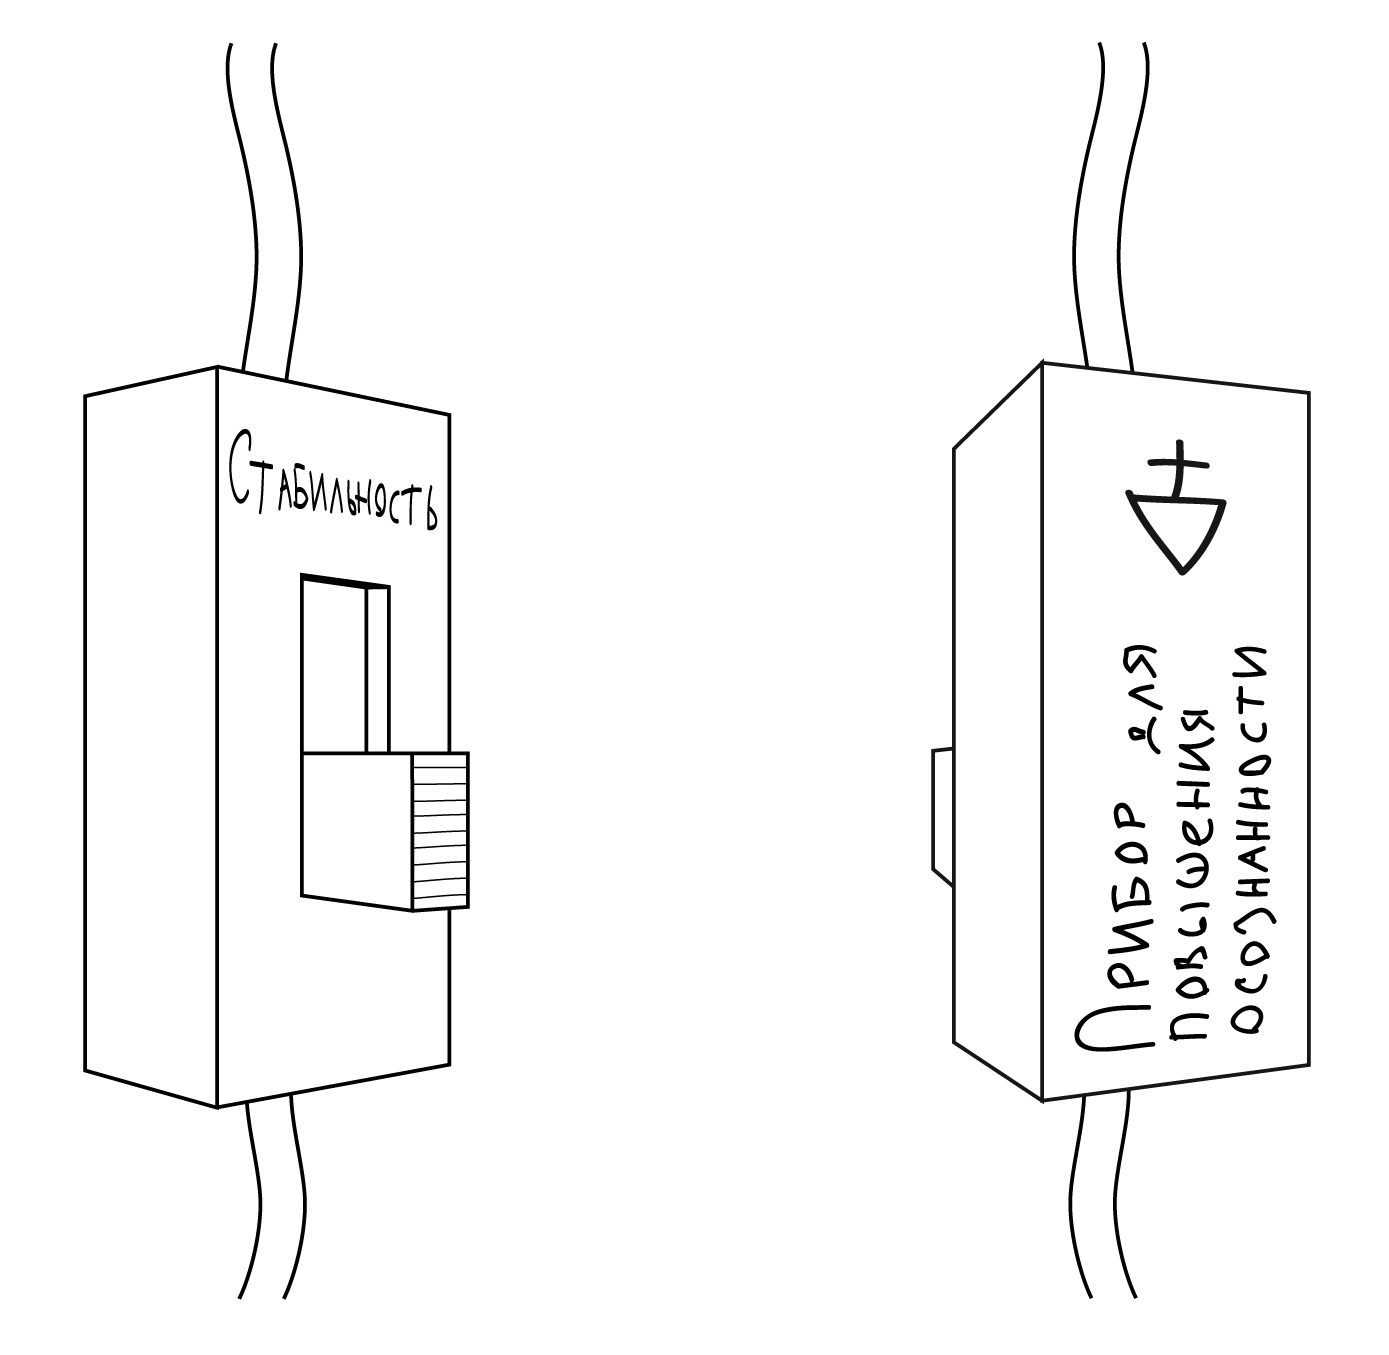
\includegraphics[width=0.8\textwidth]{ris111.png}
\end{center}
\captionsetup{figurename={Рисунок}}
\caption{}
\label{sitem}
\end{figure}

\clearpage

Что делать:
\begin{enumerate}
\item Находим/покупаем такой переключатель.
\item Пишем с одной стороны кнопки <<стабильность>> (именно в эту сторону мы будем её переключать).
\item С другой стороны самого выключателя (сзади, то есть) рисуем алхимический символ трансмутации~--- грубо говоря, он символизирует <<изменение>>, в нашем случае это оптимально, и ещё раз повторю: никакой мистики, просто этот символ прекрасно воспринимается подсознанием, не верите — читайте Юнга, где он разложил всю Алхимию на символы бессознательного, от чего просрался кирпичами, да и не только он. Также там пишем <<Прибор для увеличения осознанности>>. Ну, в общем, см. рисунок \ref{sitem} 
\item Носим его всегда с собой в кармане, время от времени рассматриваем, представляем как во сне мы его включим, и всё станет ярче и стабильнее. 
\item Периодически IRL включаем, тут надо вспомнить, как играли в детстве. Помните, как бегали с деревянными игрушками, представляя, что это реальный пистолет или меч? Помните детскую радость от такой игры? Вот надо чего-то подобного добиться; включаем и представляем, как всё стало ярче и <<веселее>>, смотрим на окружающее как будто в первый раз, отчасти вызываем то же состояние, что и при просмотре руки. Так делать 2--3 раза в день. 
\item Ждём ОСа, если повезёт, то по сюжету нажмём на эту кнопку, ну или после осознания лезем за ней в карман. 
\item ???
\item PROFIT
\end{enumerate}

Вот какбе и всё. Но ещё раз подчеркну: обычно такие вещи каждый делает сам под себя, методом проб и ошибок и на более поздних стадиях. 

Первый раз я решил попробовать придумать некий <<базовый универсальный рецепт>>. Так что ничего не гарантирую, более того, может быть, что вас сразу выкинет, как его в ОСе включите. В теории работать должно хорошо, но на практике хрен знает.

Так что тут испытания чисто добровольные. Хотите~--- делайте, не хотите~--- не надо, или попробуйте сделать что-то под себя индивидуально, благо как делать и что это может дать вы уже знаете. 

Удачи. Ня :3 



\chapter{Техники на крайний случай}
Итак, что мы имеем:
\begin{itemize}
\item Ты не запоминаешь снов и не можешь осознаться.
\item Ты спишь в одной комнате с родственниками, поэтому всякие эксперименты со звуком отменяются.
\end{itemize}

Значит нафиг звук, будем работать по-другому. 

\begin{enumerate}
\item Выбери какое-нибудь место, где часто бываешь, и попробуй его внимательно осмотреть, замечая детали, план и т.д.
\item Каждый вечер пиши маленький рассказ (хотя бы в общих чертах, ну предложений 4--10) про то, как тебе приснился сон в месте, которое рассматривал.
\item Если на утро ничего не помнишь, то в дневнике пиши: <<Я вспоминаю мой сон, как вспомню~--- запишу>>. При этом постарайся поверить и прочувствовать эту фразу. 
\item Те сны, что у тебя записаны, переведи (хотя бы 3--5 штук из них) в другой формат, то есть, если писал на бумаге, то перепечатай на компе, или наоборот. 
\item Прочитай про прямые техники Радуги и попробуй поделать их.
\end{enumerate} %как-то много спискоты


\textit{(Да, в списке выше нет методик, связанных с дыханием. Но не потому, что мы о них не знаем. Напротив~--- такие методики периодически вбрасывают в треды. Однако Горшок относится с подозрением к таким вещам, что разделяет и большинство остальных участников. В общем, особо мы их не обсуждали и не практиковали, а потому и в методичке о них ничего нет~---примечание редактора)}



\chapter{Улучшение памяти}
В общем, эту технику мне рассказал очень давно один старый знакомый. Потом я на неё ещё где-то натыкался, по-моему в чём-то с Тибетом связанным, ну не суть.
 
Основная идея проста: привязка конкретных блоков знаний (например, формула, биография, столицы мира, кости человека, и т.д.; назовём это для удобства <<блок знаний>>) к объектам в воображаемой комнате. Ассоциативное мышление + заигрывание с подсознанием, тащемта :3
 
Суть такова: для начала нужно определиться с нашим воображаемым помещением; на первых порах лучше брать что-то, что хорошо знаешь IRL, например, свою комнату/квартиру, в которой живёшь. Далее надо немного потренироваться и проверить~--- можешь ли ты в деталях её представить с закрытыми глазами? Дальше лучше на примерах: нужно запомнить все кости скелета человека. Как мы это будем делать?

Определяемся, где в комнате будет скелет :3 Не в визуальном плане, а именно где будут лежать знания о нём. Допустим, что он у нас будет в шкафу. Причём ноги будут в нижнем ящике шкафа, руки в боковом, а остальное на вешалке :3 

Когда читаем про строение скелета, стараемся держать в уме, где именно в нашей <<комнате>> лежит та или иная его часть.
 
Тут сразу возникнет вопрос: <<А сколько так учить? Да и вообще, Горшок, ты хуй, если всё равно надо учить, то в чём профит?>>. На самом деле, чтобы запомнить таким образом все кости человека, достаточно прочитать раза три; тут надо понять, что термин <<запомнить>> вообще нихуя не правильный, <<запоминаем>> мы всё, что видим с первого раза, трюк именно в извлечении этой инфы, поэтому в этом упражнении упор надо делать на <<вход>> в комнату, об этом ниже. 

Итак, мы знаем, где у нас лежит скелет, и мы о нём раза три-четыре прочитали. В памяти теперь держим только то, где он находится. Через пару дней пришла пора сдавать экзамен, нам попадается билет с вопросом: <<Перечислите все кости человеческой ноги>>. Теперь самое главное~--- это тот самый <<вход>>. Закрываем глаза, расслабляемся, насколько это возможно, представляем, что стоим в центре нашей комнаты, стараемся воссоздать все мелкие детали, подходим к шкафу, медленно открываем дверь, стараемся почувствовать и представить каждое движение и тактильные ощущения от ручки шкафа, таким же образом открываем нижний ящик\ldots ВНЕЗАПНО вспоминаем и все кости, из которых состоит нога :3 <<Вспоминание>> похоже на то, как общаются некоторые NPC во сне, то самое <<понимание>> :3
 
Собственно, вот и всё. Теперь о нюансах:
\begin{itemize}
\item Конечно, желательно сначала эту технику отработать дома; ещё раз подчеркну, что важно научиться выполнять <<вход>> в комнату, в идеале вообще должно быть что-то вроде <<фазы>>. 
\item В дальнейшем можно создать несуществующую комнату. Но это занятие долгое и нудное, нужно уделять внимание деталям, например: <<Вот у того ящика слегка болтается ручка>> и т.д. 
\item Нужно размещать <<блоки>>, опираясь на ассоциации. Например, если учим биографию исторических личностей, и решили разместить их в холодильнике на полках :3, то Наполеон будет на самой нижней из них, так как он был маленьким :3 Но тут всё индивидуально, подбирать ассоциации надо под себя самому. 
\item <<Лимита>> запоминания и времени хранения тут нету, пока помнишь что/кто где лежит, всегда сможешь вспомнить детали. 
\item Важно уловить <<суть>> упражнения и отточить навык выхода. Поначалу может не получаться, нужно просто чуть-чуть упорства. Как уловишь идею, то учить больше вообще ничего не придётся. При хорошей прокачке навыка, не нужно будет даже глаза закрывать, просто вспоминаешь, где нужный <<блок>> лежит, и тут же приходят все воспоминания по нему. 
\item Не нужно пытаться вспомнить насильно, не нужно вообще в процессе извлечения <<блока>> о нём думать; ты в комнате, и ты просто лезешь в шкаф <<взять>> вещь. Воспоминания придут сами.
\end{itemize}



\part{ Теория}


\chapter{Вопросы восприятия}




\section{Модальности восприятия}
Выскажу кое-какие мысли по поводу успешности/без\-ус\-пеш\-нос\-ти тех или иных прямых методов вхождения в ОС: графического и <<мелодии сна>>.

Вообще, в психологии в целом и НЛП в частности существует несколько модальностей восприятия, среди них выделяют три главные: визуальную, аудиальную и кинестетическую. У человека может быть ведущая и первичная модальности; ведущей модальностью человек пользуется для хранения и извлечения информации из памяти, первичная же используется для обработки (как лингвистической, так и <<внутренне-диалоговой>>) этой информации. Соответственно, ход мышления и эффективность образов той или иной модальностей существенно разнится от человека к человеку.

Я пришел к выводу, что эффективность того или иного способа вхождения в осознанный сон зависит от того, человек с какой ведущей модальностью пользуется этим способом. Поясню на примере.

Например, для некоего абстрактного Васи ведущей является аудиальная модальность. Он лучше хранит в памяти звуки: разговоры, мелодии, вообще~--- информация запоминается им последовательно, в том порядке, в каком он ее <<услышал>>. Предположим, что Вася~--- <<чистый>> аудиал, то есть и первичной модальностью для него является аудиальная (он и выражает свои мысли, используя категории аудиальной модальности). И если такой Вася воспользуется графическим методом вхождения в ОС (то есть будет насиловать свой мозг, натужно представляя доску и грифель, выводящий цифры), скорее всего, он потерпит неудачу, т.к. предполагаемые методом действия плохо соотносятся с его модальностью, с его привычным способом мышления. Для такого Васи, как мне кажется, гораздо эффективнее сработает мелодия сна~--- особенно, если Вася качественно поработает над созданием якоря <<мелодия=ЭТО СОН, БЛЕАТЬ>>.

Надеюсь, пример достаточно ясен.
 
Теперь, собственно, мысль, к которой я подводил: прежде, чем начинать задрачивать то или иное упражнение, и говорить потом: <<Ничего не работает, упражнение плохо зделали тупо!>>, выявите, а стоит ли его вообще вам делать! Может, с упражнением для другой модальности у вас выход состоится в первую же ночь.

Чтобы узнать больше о модальностях и выявить свою первичную и ведущую модальности, рекомендую <<НЛП. Практическое руководство>> (\url{http://flibusta.net/b/141203}) от Гарри Олдера и Берил Хезер.




\section{Об излишней уверенности в собственной модели восприятия}
\begin{tikzpicture}
\node [fill=futababack,rounded corners=5pt,text width=13cm]
{
Один раз рассказал про ОС (радость же)~--- высказали подозрение на неправильную работу мозга.
\smallskip
Как же меня поражает это мастерское умение делать выводы из\ldots НИЧЕГО.
};
\end{tikzpicture}

Стереотипы + железобетонная уверенность в своей модели восприятия. Это отчасти даже нормально, таким людям надо просто подыгрывать, это очень забавно и полезно :3 

Ну вот, например, появилась тян, которая увлекается ОСами, так вот, родителям не надо это говорить, лучше выбрать плюсы которые не конфликтуют с их моделью. Например, рассказать, какая она воспитанная и как вкусно умеет готовить :3 

Ненависть, которые многие испытывают к тем, кого часто называют <<быдло>> (очень, кстати, не люблю это слово)~--- это следствие своих же проблем; это как троллинг, ведь разыгрывая какой-либо спектакль и получая в ответ тонны ненависти, ты не заботишься о чужом мнении, правильно? Тебе банально похуй. Любая негативная эмоция, не связанная с прямой угрозой жизни~--- следствие внутреннего конфликта. 

\medskip

"--* Он тупой быдлогоп, как можно быть таким убогим и недоразвитым? 

"--* Зато он ебёт тян и может убрать меня прямым правой.

\medskip

"--* Она жирная взрослотота, думающая только о нямке и детях, а ещё считает, что каждая девушка должна рожать детей\ldots FUUUUU! какая она отсталая, я не такая, я-то умнее.

"--* А так хочется иметь парня с которым захочется завести семью\ldots. % плохотупо, переписать

\medskip

"--* Да что он меня жизни учит, блеать? Сам слесарь пропитый, а чего-то талдычит, я вон в интернете сижу, у меня доступ к знаниям всего мира.

"--* Однако я хикки-задрот, а то, о чём он рассказывает, для меня недостижимо, но желанно.

\medskip

"--* Айфон~--- говно!!!11одинодинодин. 

"--* Но купить то хочется, блеать. 

\medskip

Думаю, идея понятна. Такой получился небольшой экскурс в психологию, надеюсь, ненависти не вызовет. % oche надеюсь 




\section{Про веру} 
\begin{tikzpicture}
\node [fill=futababack,rounded corners=5pt,text width=13cm]
{
Ну я скептик, да. Если бы не Лаберж с его научным подходом, я бы ОС никогда и не заинтересовался.
};
\end{tikzpicture}

\medskip

Понимаешь, какое дело, есть скептицизм здоровый, а есть не очень :3 Нет-нет, я не хочу тебя обидеть или что-то навязать. Но, просто вот такое наблюдение~--- у самых суровых скептиков хуже всего получается работать с ОСами :3 

Конечно, не надо во всё слепо верить, я к этому и не призываю, но вспомни: надеюсь, читал мою статью о <<жидкости сознания>>, на самом деле, без разницы, является ли человек <<суровым скептиком>> или <<суровым верующим>> :3 Итог в области психологических экспериментов и практик один. 

То есть любая уверенность в чём-то на 100\%~--- это лишний стимул <<защитным механизмам>> предотвратить появление чего либо, что способно потрясти твою уверенность. 

Пойми меня правильно, скорее всего, сейчас ты испытываешь некоторое негодование :3 Но, как это смешно не звучит~--- в области работы с психикой вера играет первостепенное значение :3 




\section{О сложности моделей}
Вот я считаю, что не нужно сильно ударяться в какие-либо сложные модели, хотя это может, так сказать, <<проф. привычка>> :3
 
Я уже вроде говорил, что <<Если человек понимает какую-либо тему, то он может её объяснить ребёнку восьми лет (или шести, точно цитату не помню,  лол)>>. Я всегда стараюсь следовать этому правилу. Более того, иногда полезно пересмотреть свои концепции с этой точки зрения. Порой излишние логические конструкции только мешают. 

Представь себе маленький шарик~--- это вот идея, ты её видишь и понимаешь. Но сознание требует огранить её в какую-либо модель, и ты над этим шариком начинаешь строить сложные металлические конструкции/выводы, возводишь целые небоскрёбы и в результате под ними шарика часто становится не видно (и ему грустно и печально, что о нём забыли, уааа, хнык). 




\section{О стремлении быть лучше других}
\begin{tikzpicture}
\node [fill=futababack,rounded corners=5pt,text width=13cm]
{
\textcolor{futabaq}{>Очень многих одолевает соблазн писать о чём либо, не имея в этой сфере \textbf{практических} успехов, и это мега-фейл.}

\smallskip

Да уж\ldots

Мне кажется, человек просто склонен делать выводы и заключения, при этом не имея на то вообще каких-то причин и мотивов, и достаточных знаний для того. Ну тут, возможно, проявляется стремление Эго все упорядочить и вписать в существующую модель мира.

В итоге кругом выдающиеся специалисты, с легкостью ведущие беседы о работе мозга, квантовой механике и прочем.

Проблема в том, что у меня от этого постоянный баттхерт, который я не пойму, как лучше реализовать. Ну, может, с опытом пройдет.
};
\end{tikzpicture}

\medskip
И ещё стопицот всяких других вещей. Это нормально, желание быть или хотя бы выглядеть умнее, сильнее, мудрее и т.д., чем остальные люди, вполне естественно, главное~--- просто его в нужное русло направлять, и не вестись на всякие самообманки :3 

Тут просто есть такой нюанс, что человеку для <<игр>> зачастую напарник и не нужен :3 

Если интересно, то почитай: Вадим Демчог~--- <<Самоосвобождающая игра>> (\url{http://flibusta.net/b/172573}). Он крайне занятно эту тему (театр одного актёра) освещает. 

А вот баттхёрт это плохо, любую попоболь надо тщательно исследовать.
 
Вообще, тут хорошо работает позиция <<стороннего наблюдателя>>. То есть ты не зацикливаешься на <<Вот он урод, нихуя не знает, а строит из себя гения>>, а смотришь с точки зрения <<Почему он так делает? Зачем? Что ему это даёт?>> ну и т.д. Ну и, кроме того, тут можно ещё словить фейл на тему <<просирания инфы>>, вдруг тот человек что-то дельное вещал? Вообще, в любом случае можно выиграть:
\begin{enumerate}
\item Он вещает что-то дельное~--- ты об этом узнал.
\item Он вещает хуиту~--- ты понял, что он так считает, и побольше о нём узнал. 
\end{enumerate}

Всегда надо стараться из всего извлекать профит. Причём, чем менее, на первый взгляд, <<профитная>> ситуация, тем ценнее в итоге будет полученная инфа. Читать умные книжки, где всё разжёвано, может каждый, а вот находить знания в обыденных ситуациях намного сложнее :3 




\section{Источники информации мозга}
\begin{tikzpicture}
\node [fill=futababack,rounded corners=5pt,text width=13cm]
{
Как-то раз мне снилась обычная слабозапоминающаяся каша. Долго. Я потерял ко сну интерес и смотрел <<в пол-уха>>. Потом что-то изменилось. Насторожился, пригляделся. Значит, вижу такую картину: я на своей кухне, играю с ножами. Они красиво блестят в слабом свете ночника. И я при этом такой довольный, что чуть ли не хихикаю вслух. Отметил про себя, что такое поведение для меня нетипично (имею в виду труд :3). Пытаюсь оглядется и замечаю что я выше чем есть на самом деле, при этом не вижу ног, да и вообще всего тела, стараюсь разглядеть~--- не выходит. Думаю ладно, образ шарообразного существа с невидимыми тентаклями мне тоже нравится. Дальше хреново помню\ldots по моему, наигрался и пошел спать.

Жил я тогда не один: я, мать и ещё один мужичок с нами сожительствовал (лол, ну и фраза получилась). На утро выяснилось, что все ножи заточены. Два дня мы удивлялись как же так. Потом мужичок признался что проснулся ночью поссать и что-то ему не хотелось спать, решил так подшутить. 

Не вдаваясь в детали я бы сказал, что это было в соседней квартире. Лунатизмом не страдаю, так что даже не знаю как бы я это мог подсмотреть/подслушать.
};
\end{tikzpicture}

\medskip

Насчёт слуха я выше писал, ты в теории можешь слышать сейчас, например, отзвук того, как разбилась бутылка через дом напротив. Более того, ты можешь по этому отзвуку сказать, с какого этажа её выбросили, более того, лол, ты можешь даже сказать, в каком настроении был тот, кто её выбросил. %шо за ересь 

Точнее мог бы, так как вся необходимая информации у тебя есть, но сознание так устроено, что отсеивает лишнее, хотя <<помнишь>> ты все-все-все звуки, запахи, и прочее, что когда-либо воспринимал. Просто связи частенько бывают крайне неоднозначными.

Вот, допустим, идёшь ты с другом в людном месте по своим делам, вы общаетесь и не обращаете внимания на окружающие разговоры и прочее. А вдалеке от вас два террориста в тихом уголке обговаривают завтрашнее место теракта. Внезапно, как раз завтра ты хотел туда сходить. Сам разговор разумом ты не услышал, слишком далеко, <<тихо>>, и вообще ты занят, с другом общаешься, ну и побочные шумы мешают. Однако всё происходящее, все мельчайшие звуки, вообще ВСЁ, что ты слышишь, грубо говоря, <<пишется>> и, кроме всего прочего, анализируется.

А дальше всё зависит уже от особенностей твоей психики: ночью может быть кошмар с намёком <<нехуй туда идти>>, или просто <<плохое предчувствие>>, ну и прочее. Увы, человек, в отличие от животных, своим инстинктам и предчувствиям доверяет редко. 

Собственно, как-то так. В этом-то как раз один из потенциальных профитов от ОСов~--- возможность работать с такими массивами информации в обход сознания, нагло юзая при этом вычислительные мощности мозга :3

\bigskip

\begin{tikzpicture}
\node [fill=futababack,rounded corners=5pt,text width=13cm]
{
Но тогда все порнографические сны мне снились тоже не просто так, а потому что кто-то где-то трахался.
};
\end{tikzpicture}

\medskip
Не факт, сюжет снов может строиться из разных моментов. Может отражать тяжёлое переживание, <<предчувствие>> чего-то, показывать проблемы в психике и прочее. Именно что-то связанное с IRL обычно ярко проявляется в случае опасности, это самые глубокие инстинкты и архетипы, но такие сны обычно сложно не заметить.
 
Заточка ножей (sic!) ночью, по-моему, достаточно странное событие, чтобы отобразить его в сюжете, но недостаточно <<стрёмное>>, чтобы тебя разбудить. Этакая <<балансировка>> между сигналами <<Опасность!>> и <<Просто странный шум>>.

Слух у меня очень избирательный, я вот, допустим, сколько раз засыпал у себя в квартире во время <<посиделок>>, и плевать мне на музыку, посторонние разговоры и прочее. Но как только кто-то открывает входную дверь в квартиру, я тут же моментально просыпаюсь. 

Или, например, мать с ребёнком. Она может (если устала) заснуть при включенном телевизоре, но моментально проснуться даже от слабо доносящегося плача своего ребёнка. 

Это всё на уровне инстинктов. Причём в список <<алярмов>> могут добавляться новые, или просто в течении жизни под воздействием внешних факторов, или ставиться специально, начиная от умения просыпаться в метро именно на нужной тебе остановке, и заканчивая, например, бросанием ножа во входящего в комнату без стука. Кроме шуток, кстати, знаю человека, которого очень вредно для своего здоровья будить прикосновением~--- он сразу на автомате бьёт в зубы. Тяжёлое, гм\ldots детство способствовало выработке такого рефлекса. 


\section{Откуда NPC знают, что ты нравишься девушке}
\begin{tikzpicture}
\node [fill=futababack,rounded corners=5pt,text width=13cm]
{
\textcolor{futabaq}{>Например, <<Нравлюсь ли я вот той тян?>>}

\smallskip

Имеется в виду конкретная тян из материального мира? Если да~--- откуда моему подсознанию знать, нравлюсь ли я ей?
};
\end{tikzpicture}

\medskip
Из настоящего, да. Откуда знать\ldots Ну, помнишь, я писал, что информация запоминается вся? Это и запахи, и движения глаз, и мельчайшая мимика лица. Отсюда, например, некоторые люди вызывают симпатию или антипатию. Например, увидел на улице человека и стало жутко, а почему? Что в нём не то? Обычный человек, ан нет, подсознание обработало его детали (всё, что связанно с опасностью для жизни, оно делает очень быстро), обнаружило его пластику движений, его быстрый и цепкий взгляд, и ещё кучу нюансов, после чего сделало вывод, что человек опасен, так как имеет боевую подготовку.

Сознание же получает только <<итого>>, все эти расчёты обычно проходят мимо него. Ну и часто, конечно, они игнорируются, подключается логика, размышления и прочее, однако <<первое впечатление, как правило, самое верное>>.

\begin{shaded}

\begin{center}
\Large\bfseries{Кулстори: бессознательное определение симпатии}
\end{center}

В прошлом году я у меня особо обострились ЕОТ-переживания, вполне обычное дело. В то же время началась очередная полоса успехов на поприще осознанных сновидений, чем я решил воспользоваться. Хорошенько углубился в одном из ОС и спросил у NPC: <<Любит ли меня \textit{одна тян}?>>. Ответ оказался на удивление прямым и понятным: <<Нет, это маловероятно>>. Огорошенный им, я решил покончить с этими пиздостраданиями и через пару недель подловил ту тян и признался ей. Увы, NPC был прав: никаких чувств девушка ко мне не испытывала. 

Зато потвердилась теория из треда. Главное~--- предварительно углубиться, иначе вместо ответа будет бессвязный поток речи.

\end{shaded}



\section{Влияние ОС на сюжеты снов}
\begin{tikzpicture}
\node [fill=futababack,rounded corners=5pt,text width=13cm]
{
Кто-нибудь обратил внимание, что сны постепенно стали более\ldots бытовыми, что ли? С момента начала ведения дневника~--- фантастики всё меньше, а разговоров с преподами больше.
};
\end{tikzpicture}

\medskip
У каждого по-разному. Вообще, бывает, да, не могу сказать, <<хорошо>> это или <<плохо>>, скорее, это следствие самокорректировки психики. Как бы даже простые ОСы, без всяких хитрых шаманств, уже самим своим фактом вызывают <<обратный эффект>> отладки. 

Если это попытаться объяснить на примере, то выйдет хуита, но я попробую: ВНЕЗАПНО подсознание смотрит на само себя со стороны через осознание во сне, начинает люто срать кирпичами от этого пиздеца и быстренько начинает наводить в себе самом порядок. 

Да-да, звучит не очень, но я тут упоминал про ЭЭГ с обратной связью, например. Когда человек слушает музыкальную обработку биоэлектрической активности своего мозга, мозг начинает бешеными темпами устранять всякие баги; доходило до излечения лёгких форм аутизма.




\section{О мотивации}

Ввиду участившихся запросов и жалоб на тему <<нет мотивации делать ОСы; нет мотивации вообще что-то делать; нету цели в жизни>> и т.д. я решил запилить этакую общую статью о проблемах с мотивацией.

Прежде чем начать, предупреждаю, что многое ниже написанное может взывать лютое отторжение и недоверие, а также показаться крайне банальным. Временами банальные вещи бывают очень полезными :3 Так что прошу читать написанное ниже вдумчиво и не отмахиваться от написанного. Подчеркну, что эта статья не для тех кто <<нормально занимался а потом надоело>>, она для тех, у кого по жизни проблемы с мотивацией, целями, интересами и прочим стандартным набором хикки-битарда :3

Ну, поехали.

Сначала немного теории.

Современный образ жизни в более-менее крупных городах закладывает весьма специфическую <<основу>> психики. Отсутствие нормального обучения (в школе и дома) вместе с наличием интернета приводит к формированию такого говна, которое я называю <<самокольцевание>>. Суть крайне проста: ввиду отсутствия необходимости чего-либо добиваться (а то и вообще работать в принципе) человек погружается сам в себя, у него нет доступа к информации <<извне>>, так как знакомые все одного круга, интернет-ресурсы тоже, никаких изменений в жизни не происходит, увлечения чем-то новым обычно длятся пару недель, чётких целей на тему <<чего я хочу>> нет, так как нет мотивации, причём мотивации нет на глубинном уровне, человек просто не понимает зачем и как чего то добиваться. Знакомая картина, да? :3

Так вот, это приводит к появлению этакого <<кольца>>. Человек сам по себе доволен тем, что он есть. Это, кстати, очень сильно поддерживается подсознанием, так оно всегда стремится с покою и стабильности.

Но это ещё полбеды. Вторая половина ~--- отсутствие физического воспитания, не в плане порки и прочего BDSM, а в плане развития тела и занятий спортом. Стоп-стоп-стоп, не надо сразу меня нахуй посылать, да, знаю, что быдло, но сначала прочти дальше. 

Итак, зачем же в современном технологическом мире, где можно получать бабло и девок сидя дома за компом, заниматься, например, бегом или просто общими физическими упражнениями, не говоря уже о спорте?

Начнём с ОФП (Общая физическая подготовка). Во-первых, это биохимия, а она, сцуко, личность. В процессе упражнений мозг постепенно получает от них удовольствие, это природный антидепрессант и стимулятор, и поверь мне, природа его нам дала не зря. Во-вторых, это укрепляет здоровье, а здоровье это не только <<болит/не болит>>, оно ещё и напрямую влияет на работу мозга и психику.

Теперь про спорт. Первая мысль~--- <<Зачем мне это надо? Зачем мне с кем то соревноваться?>>. Ага\ldots можно продолжить: <<А зачем мне ОСы? А зачем мне девушка? А зачем мне работа?>>, чуешь, да? Спорт, как и серьёзные занятия ОФП, прописывает в психике новую фичу~--- удовольствие от преодоления препятствий, стремление быть лучшим, а главное~--- удовольствие от победы и достижений. Именно эта шняга двигает этот мир, няша, и закладываться она должна в детстве или в худшем случае, в переходном возрасте.

Но вместо этого, обуреваемый возрастным пиздецом в голове, человек идёт на лурк, например, и понимает, что всё это <<социоблядство, быдлизм, небылизм, альфизм>> а психика-то и рада такое принять! Ну ещё бы! Ведь ничего не надо делать, не надо что-то в жизни менять, можно тихонечко сидеть и просто быть, утопая в самом себе любимом :3

Щито же делать? Призывы вроде <<Будь мужиком!>> понятны и очевидны, но вот как-то оно лениво и не хочется. Понимаю, поэтому буду давать практики в порядке возрастающей сложности.

\begin{enumerate}
\item Займись ОФП (бег, подтягивание, приседание, отжимание, пресс). Начать можно с бега, просто выйди утром или вечером и побегай в парке. Да, первый раз нужно превозмочь и выйти из дома, но уже после первой пробежки тебя ждут интересные ощущения :3
\item После того, как осилил первый пункт и уже хотя бы месяц чем-то занимаешься, не пожалей время, всё равно ты его, скорее всего, просираешь, займись каким-нибудь спортом. Найди секцию по чему угодно и начни что-то делать, неважно что, хотя бы плавание. Лично я очень рекомендую боевые искусства, но на такое решится тяжело.
\item Расширяй круг общения, входи в другие круги. Если ты весь такой умный, то иди на сайт бодибилдеров например, и с ними общайся, хотя лучше, конечно, делать это в реале.

Я знаю что ты сейчас подумал. Поверь мне, неприятие общения с не такими как ты~--- это всего лишь уловка твоего подсознания, так как оно, напомню, очень не хочет меняться, всю жизнь вы с ним были такими стабильными, с чёткой картиной мира и прочим, и вдруг ты его зачем то тащишь в незнакомый социум. Но постепенно начнутся изменения: общаясь с другими, не такими же как ты, людьми, ты общаешься не только сознательно, но и на уровне бессознательного восприятия. Начнутся положительные (в нашем случае) изменения в психике, постепенно ты будешь расширять свой кругозор, а если люди ещё и волевые, то внезапно ты и сам приобретешь различные стремления, а главное, умение к чему то стремится в принципе.

Нет, ты не потеряешь <<себя>>, это будет просто как добавление в базу данных новой информации. Грубо говоря, подсознание и радо бы тебе помочь, но оно просто не знает что такое, например, <<желание чего-то достичь>>. Пример очень условный, но надеюсь, мысль ты понял.
\item Пробуй новое, ставя при этом цель. Тут надо дать волю своему социоблядству. Например: <<Я не просто буду делать фигурки из дерева, а сделаю такую, чтобы у всех, челюсть отвисла>>. Учись ставить и добиваться конкретных целей, а главное, не стесняйся получать от этого удовольствие и хвалиться своими достижениями. Один из самых вредных комплексов это <<Меня не интересует признание и чужая похвала/восхищение>>. Ещё как, блджад, интересуют, в тебе это на уровне биохимии заложено, не нужно себе врать, и тогда всё будет ня :3 Оптимально сочетать этот пункт с прошлым, например, займись танцами :3

\item Это практика для тех, кто уже чего-то добился, но всё равно есть чувство, что <<Что-то тут не так>>. Я называю её <<перезагрузка>>. Едешь в домик в деревне, или с палаткой в лес, минимум на неделю, один, без книг/телефона/ноута и т.д. То есть без всяких источников информации. С собой кроме еды/воды и снаряжения нужно взять только много тетрадей и пару ручек.

Этот месяц ты будешь думать о себе и о своей жизни, записывая всякие приходящие мысли, размышления, идеи, гуляя по лесу и купаясь в речке и т.д.

Просто? Очень, но работает на отлично. Я гарантирую, что вернешься ты совсем другим человеком, намного более счастливым и целеустремлённым.
\end{enumerate}

Есть ещё и другие практики, но их полезно додумать самому, благо базу я, надеюсь, дал.

Самое сложное~--- сделать первый шаг, дальше пойдёт легче и постепенно ты научишься себя мотивировать, появятся устремления, умение добиваться поставленных целей ну и ставить их в принципе :3



\chapter{Глубины бессознательного}



\section{Архетипы}

Психика~--- очень сложная штука. Приблизительно 40 000 000 000 клеток мозга, каждая из которых обладает тысячами связей: нейронная сеть неимоверной сложности; человек еще не скоро поймет, как она работает.

Психика хостится на этой сверхсложной биомашине, и где-то в ее дебрях, помимо огромного количества служебных <<программ>>, связанных с физиологией, <<выполняется>> обширный набор программ, называемый <<сознанием>>: пачка обслуживающих потоков~--- они интерпретируют сигналы, пришедшие от органов чувств, следят, чтобы сознание не оказалось перегруженным информацией, отсеивая слабый сигнал (механизм, называемый <<порогом сознания>> или <<цензором>>); механизм <<действия>>, который преобразует намерения в сложный набор нервных импульсов, приводящих в движение мышцы; речевые мыслительные потоки~-- внутренний голос или голоса, внутренний диалог; образные потоки~--- картинки, звуки из памяти или воображаемые/компилированные образы, мыслеформы; чувственный, эмоциональный фон~--- самовосприятие нейронной сети своего состояния (возбужденное, подавленное, защитное и т.д.); еще множество вещей можно отнести к осознаваемой части психики. Некоторые <<программы>> лучше осознаются, некоторые хуже, это зависит и от функции <<программы>> (например, процесс пищеварения не осознается совершенно, хотя может; процесс дыхания можно сделать осознаваемым и управлять им; на процесс серцебиения повлиять напрямую не удастся) и от того, находится ли поток в поле сознания.

На понятии поля сознания стоит задержаться и объяснить его подробнее. Психика, как уже было сказано, устроена очень сложно, но приблизительно (крайне приблизительно) представить ее себе можно в виде шарика неоднородной жидкости, который висит в пустоте. Вещество похоже на жидкие кристаллы~--- постоянно играет, меняет структуру в зависимости от сигналов снаружи и внутренних процессов. Поле сознания~--- это лучик света, который подсвечивает небольшую часть этой сферы. Процессы, попавшие в светлое пятно, видны хорошо; процессы, идущие рядом или чуть глубже оказываются в полутени; там же, куда лучик не дотягивается, кромешная тьма бессознательного, что там происходит~--- неизвестно.

У лучика несколько режимов работы (у сознания~--- несколько состояний):

\begin{enumerate}
\item Концентрированный свет~--- яркое пятно: концентрация, сознательная деятельность, сужение сознания (соответствует бета-ритму мозга);
\item Рассеянный свет~--- большая площадь охвата, но слабая освещенность: медитация, гипнотическое состояние, дрема, полусон, сновидение, ОС, расширение поля сознания (соответствует альфа-ритму мозга);
\item Луча нет~--- кромешная тьма: полное отсутствие сознательности, смерть, фаза глубокого сна (соответствует дельта-ритму мозга).
\end{enumerate}

Это очень простая классификация, более строгую можно найти в трудах физиологов.

Первый режим~--- обычное сознательное бодрствование.

Второй режим~--- отладочный. Поскольку психика~--- сложный механизм, а чем сложнее механизм, тем чаще он ломается, то нужны средства, чтобы его ремонтировать; особенно тщательно нужно беречь процессы сознательные, потому что это новейшее достижение природы. Средств, как защитных, так и восстановительных, у психики предостаточно (шаманские ритуалы, религиозные практики, медитация, гипноз, различные виды терапии, с приминением веществ и без). Одним из самых доступных любому человеку средств для отладки внутренних багов являются сновидения. Через них осуществляется компенсаторное воздействие на сознание, отправка сигналов бессознательного, отчеты о внутренней неосознаваемой работе по обработке жизненного опыта, репорты об ошибках и проблемах и много чего еще. ОС позволяют более осознанно подойти к анализу проблем, избежать примитивной, животной реакции, первобытного страха, привнести в сумеречный мир без границ и очертаний рассудок и логику, выстраивать внутренний <<плацдарм>>~--- более-менее реалистичную площадку (комнату, дом) для облегчения внутреннего путешествия.

Третий режим~--- обслуживающий или восстановительный. Сознание полностью выключается, мозг отдыхает от мыслительной деятельности, работает на <<пониженных оборотах>>, обработчики памяти записывают свежую инфу и т.д. Однако это не значит, что бессознательное бездействует.

Возвращаясь к аналогии с подсвеченным жидкокристаллическим шариком, психику можно разделить на три зоны:

\begin{enumerate}
\item Сознательная часть, самая яркая;
\item Затененная часть, осознаваемая частично, подсознательная часть;
\item Кромешная темнота~--- бессознательное.
\end{enumerate}

Как уже было сказано, в психике присутствует огромное количество условных потоков обработки/выдачи информации, большая часть которых не осознается. Группы этих потоков образуют комплексы (не в отрицательном смысле, а в иерархическом). Наиболее осознаваемая группа потоков отождествляется с сознанием.

Назревает вопрос: если сознание в самом деле только часть психики, то что же таится там, в бессознательном?

Во-первых, память. Огромное количество информации, даже не преодолевшей порог сознания, бережно записывается. Забытая естественным образом или намеренно информация, комплексы разной степени сложности, от простеньких идей, до нуменозных образов. Самые глубинные и многогранные комплексы назвали Архетипами. Что такое Архетип?

Чтобы ответить на этот непростой вопрос, придется еще порассуждать на тему структуры психики.

Во-первых, само бессознательное можно разделить на <<личное>>~--- личная память вне поля сознания, системы конденсированного опыта (термин Грофа, введенный им в <<Данных исследований ЛСД>>), подавленные, забытые воспоминания и т.п., и <<коллективное>>~--- вместилище первообразов, присущих всем людям (и, наверняка, высшим животным тоже).


\begin{quotation}
Коллективное бессознательное содержит в себе все духовное наследие эволюции человечества, возрождаемое в структуре мозга каждого индивидуума. Сознательный ум (mind)~--- это эфемерный феномен, который выполняет все провизорные адаптации и ориентации, и по этой причине его функцию лучше всего сравнить с ориентировкой в пространстве. Напротив, бессознательное служит источником инстинктивных сил души (psyche), а также форм или категорий, их регулирующих, то есть архетипов. Все самые яркие и мощные идеи восходят исторически, к архетипам. Это особенно верно в отношении религиозных представлении хотя центральные понятия науки, философии и этики также не составляют исключения из этого правила. В своем нынешней виде они представляют собой варианты архетипических представлений, созданные посредством их сознательного применения и приспособления к действительности. Ибо функция сознания заключается не только в осознании и усвоении внешнего мира через врата наших чувств, но и в переводе мира внутри нас в зримую реальность. \sourceatright{К. Г. Юнг <<Структура души>>}
\end{quotation}


Во-вторых, если рассмотреть устройство мозга, легко обнаружить, что в нем присутствуют как системы очень древние, которые можно найти и у первых хордовых, так и сравнительно современные, например, кора мозга. И если сознательная деятельность связана с современными подсистемами мозга, то бессознательная и, особенно, коллективная его часть больше связаны с более древними подсистемами. Древний человек, у которого еще не было выраженного критического сознания, поскольку не было развито подходящих структур в мозге, мыслил более примитивно. Не существовало очевидного теперь нам разделения на внешние процессы и внутренние, поэтому важные внутренние и внешние события при их многократном повторении запечатлелись в виде базовых первопредставлений, неких матриц восприятия. Например, восход/заход солнца, цикл день/ночь древним человеком трактовались как проявление божественных сил и со временем мифологизировались, как и многие другие вещи; такие понятия, как <<мать>>, <<отец>>, <<сын>>, <<семья>>, <<любовь>>, <<герой>>, <<бог>>, <<душа>>, <<солнце>>, <<луна>>, <<дерево>> и т.д., их великое множество~--- все они закрепились архетипически.

Проявление, действие и значимость этих образных базовых структур трудно переоценить. Например, математика обязана своим появлением осознанию философами древности архетипических образов числа, пустоты, вечности, бесконечно большого и бесконечно малого. Знаменитый миф о герое, тянущийся корнями к солярному мифу и архетипическому закреплению солнечного каждодневного цикла, используется до сих пор в кино и литературе. Современная вариация мифа о герое обычно выглядит так: неудачник получает супер-силу, справляется с проблемами и становится счастлив. Архетипический образ диссоциации личности, первобытный страх <<потерять душу>> сегодня выражается в идее массого психоза, когда множество людей теряют сознательность, что проявляется в многочисленных произведениях про зомби, которые пользуются бешеной популярностью. И так как эти образы встречаются повсеместно, они очень сильны.

Архетип~--- это форма, идея, матрица, кристаллическая решетка для бессознательного содержания. С некоторыми из этих образов наверняка встретится каждый, кто занимается ОС. Я постараюсь дать краткую характеристику наиболее часто встречающимся архетипическим образам и посоветую, как себя вести при встрече.

\begin{center}
\bfseries{Тень} 
\end{center}


\begin{quotation}
Тот, кто смотрит в зеркало вод, видит прежде всего собственное отражение. Идущий к самому себе рискует с самим собой встретиться. Зеркало не льстит, оно верно отображает то лицо, которое мы никогда не показываем миру, скрывая его за Персоной, за актерской личиной. Зеркало указывает на наше подлинное лицо. Такова проверка мужества на пути вглубь, проба, которой достаточно для большинства, чтобы отшатнуться, так как встреча с самим собой принадлежит к самым неприятным. Обычно все негативное проецируется на других, на внешний мир. Если человек в состоянии увидеть собственную Тень и вынести это знание о ней, задача, хотя и в незначительной части, решена: уловлено по крайней мере личностное бессознательное. Тень является жизненной частью личностного существования, она в той или иной форме может переживаться. Устранить ее безболезненно~--- с помощью доказательств либо разъяснений~--- невозможно. Подойти к переживанию Тени необычайно трудно, так как на первом плане оказывается уже не человек в его целостности; Тень напоминает о его беспомощности и бессилии. \sourceatright{К. Г. Юнг <<Архетип и символ>>}
\end{quotation}


Встреча с Тенью практически гарантирована, если заниматься снами достаточно долго.

Это набор мыслительных потоков, воспоминаний, которые мы сами в себе подавляем и не принимаем. Постепенно накапливаясь, эти потоки формируют сравнительно автономный неосознаваемый комплекс психики, который способен доставить немало хлопот. Обычно образы Тени отличаются по уровню осознанности. Если теневые процессы слабо осознаются, то Тень обычно проявляется в виде насекомых: жуков, пауков, личинок, то, что вызывают страх или непрязнь у человека. Еще один пример~--- змеи. При лучшей осознанности Тени, она облачается в символ какого-либо дикого и хищного животного: собака, волк, тигр, кабан и т.п. На самой высокой степени осознанности Тень обычно представляется человеком того же пола, что и сновидец, вызывающим множество негативных эмоций.

Задача сновидца~--- интегрировать Тень, примирится с нею, то есть с самим собой, принять самого себя и понять свои недостатки. От Тени не нужно убегать или прогонять ее, нужно понять и обнять, помириться. Звучит это довольно просто, но на деле оказывается, что сделать это весьма сложно. Тут как раз и приходят на помощь ОС, посредством которых человек интегрирует бессознательный материал более конструктивно.

\begin{center}
\bfseries{Анима/Анимус}
\end{center} 


\begin{quotation}
Анима~--- это олицетворение всех проявлений женственного в психике мужчины: таких как смутные чувства и настроения, пророческие озарения, восприимчивость к иррациональному, способность любить, тяга к природе и~--- последнее по порядку, но не по значению~--- способность контакта с подсознанием. \sourceatright{М. Л. фон Франц <<Процесс индивидуации. Общая схема духовного роста>>}
\end{quotation}

Сильные наполнения архетипа встречаются довольно редко, но тем сновидцам, кто испытывает большие проблемы при общении с противоположным полом, наверняка предстоит пообщаться с этими мощными проявлениями бессознательного.

Так же, как и Тень может иметь стадии осознанности.

\begin{quotation}
Первую стадию лучше всего символизирует образ Евы: чисто инстинктивные и биологические связи. Вторую стадию можно наблюдать в образе Елены в <<Фаусте>>. Она олицетворяет романтический и эстетический уровень, которому еще присущи черты сексуальности. Третья стадия представлена Девой Марией~--- образом, поднимающим любовь (эрос) до вершин духовной преданности. Четвертый тип символизирует Сапиенция~--- высшая мудрость, превосходящая высшие святость и чистоту. Другим символом этого уровня является образ Суламифи в Песне Песней Соломона. \sourceatright{М. Л. фон Франц <<Процесс индивидуации. Общая схема духовного роста>>}
\end{quotation}

Анима~--- архетип жизни и смерти, смысла жизни и ее непрекращющегося движения и бурления. Для жизни нет добра и зла, и она имеет как созидательное, так и разрушительное начала, поэтому встречается как в положительных образах (женщина-проводник, советчица), так и в отрицательных (ведьма, русалка, суккуб и т.п.). Намеренно искать встречи во сне с такими сильными явлениями не стоит, потому что могут вызвать панический страх, по сравнению с которым страх перед Тенью покажется несерьезным.

Как Анима является архетипом женственности в мужчине, Анимус является архетипом проявлением мужского в женщине.

\begin{quotation}
В точности как анима, анимус проходит через четыре стадии развития. На первой он знаменует простую физическую силу, например, как чемпион по легкой атлетике или мужчина с горой мышц. На следующей стадии он олицетворяет инициативу и способность планировать свои действия. На третьей~--- анимус представляет <<слово>>, зачастую реализуясь в качестве профессора или религиозного деятеля. Наконец, в четвертой~--- анимус становится воплощением смысла. На этом высшем уровне он опосредует, подобно аниме, религиозный опыт, через который жизнь приобретает новый смысл. Он придает женщине духовную твердость, невидимую внутреннюю поддержку, что компенсирует ей внешнюю мягкость. \sourceatright{М. Л. фон Франц <<Процесс индивидуации. Общая схема духовного роста>>}
\end{quotation}

Так же, как Анима, является одним из самых сильных образов в психике, символизирующий интеллект и твердость ума. И так же, как Анима, имеет положительные и отрицательные проявления.


\begin{center}
\bfseries{Самость}
\end{center} 

Редко встречается, но если встретится достаточно сильный символ или образ, запомнится на всю жизнь.

Самость~--- архетип духовной, психической целостности, просветления, высшей осознанности. Часто выступает в роли советчика и подсказчика. Своим появлением стабилизирует психику. Может проявлятся чисто символически~--- камень, мандала, шарик, крест с центральной симметрией и т.п.

\begin{quotation}
Если индивидуум достаточно серьезно и долго боролся с проблемой анимы (или анимуса) и добился прекращения отождествления с ними части своей личности, подсознание вновь изменяет характер своего влияния и выступает в новой символической форме, представляющей Самость~--- глубочайшее ядро психики. В сновидениях женщин этот центр обычно олицетворяется верховным женским образом~--- священнослужительницей, волшебницей, матерью-землей или богиней природы и любви. У мужчин он проявляется как человек, посвящающий в тайные образы или их хранитель (индийский гуру), мудрый старец, дух природы и т. д. \sourceatright{М. Л. фон Франц <<Процесс индивидуации. Общая схема духовного роста>>}
\end{quotation}

\fancybreak{* * *}

Тут же стоит сделать важное замечание: довольно часто сновидцы в треде, поверхностно ознакомившись с Юнгом, начинают видеть архетипы повсюду, то есть впадают в то, что сам Юнг называл архетипическим редуцированием и от чего частенько предостерегал. Как уже не раз говорилось, шанс столкнуться с персонифицированным архетипом во сне или ОСе очень мал, и, уж поверь мне, такое ты точно ни с чем не спутаешь. 

В то же время, для удобства в треде при описании символов своих снов/о\-со\-знан\-ных сно\-ви\-де\-ний персонажи и предметы, имеющие отношение к тому или иному архетипу, помечаются, собственно, как сам архетип. Вообще, это не лишено определённого смысла, ведь в основе всех комплексов лежит архетипическая основа, но это не значит, что какая-нибудь мелкая бага, связанная, скажем, со страхом темноты, представляет собой в ОСе <<глубокую>> Тень. Несомненно, в этой баге могут быть те или иные архетипические грани, но будет большой ошибкой принять лишь верхушку айсберга за всю его скрытую от взора громаду. Если процитировать одного из персонажей осозняши из треда, то звучит это примерно так: <<Я не Анима, но достаточно близка к ней, чтобы через меня ты мог обращаться к ней>>. Nuff said.




\section{Либидо и Мортидо}

\begin{tikzpicture}
\node [fill=futababack,rounded corners=5pt,text width=13cm]
{
В моих снах присутствует подозрительно большое количество открытых конфликтов с драками, поножовщиной, стрельбой <\ldots> Даже в школе дрался не более одного раза, вот и думаю~--- откуда во мне это всё?
};
\end{tikzpicture}

\medskip

Итак, многие слышали краем уха такой термин, как <<Либидо>>, правда, ассоциируют его исключительно с еблей, но об этом ниже. Так вот, есть ещё такая штука, как Мортидо, об этих двух крайне важных понятиях в нашей психике и пойдёт речь. 

Давайте сначала дам определения обоих этих слов. 

Либидо~--- стремление созидать. Его высшее проявление~--- создание ребёнка.

Мортидо~--- стремление разрушать. Высшее проявление~--- убийство. 

Но есть пара крайне интересных нюансов: обе эти вещи могут быть направлены как вовне (рождение ребёнка/убийство человека), так и вовнутрь (совершенствование себя/самоубийство). Важно понять, что бороться с этими вещами бесполезно, их можно представить как две постепенно заполняющиеся шкалы в РПГ, необходимо постоянно их <<сливать>> куда-либо, потому что иначе, если одна из них заполнится полностью, будет пиздец (тяжёлые психические расстройства, срывы, самоубийство и т.д.), понятное дело, что <<слив>> этих шкал происходит бессознательно и может принимать причудливые формы. 

То есть, не надо понимать всё буквально, то же Мортидо вовне может выражаться как скандалы с ближними, пакости знакомым, необоснованная НЕНАВИСТЬ к чему-либо. Вовнутрь оно принимает, например, формы курения, алкоголизма, запускания своего внешнего вида и гигиены. 

Либидо во вне может принимать форму творчества, рисования, созидания. А вовнутрь будет выглядеть, как работа над собой, например, занятие в спортзале. Это всё крайне тесно переплетается с комплексами, моделями восприятия и т.д. То есть, важно понимать, что Либидо и Мортидо это не что-то отдельное, это части огромного и сложного механизма под названием <<психика человека>>. 

Думаю, если кто-то до сюда дочитал, то рядом уже имеется небольшая кучка кирпичей. Возникнет закономерный вопрос: <<А что делать-то?>>. А почитать историю, например. Какой культ был в древности и сохранился до сих пор? Вот не поленитесь, подумайте минут 5--10, а потом читайте ниже. 

А разгадка проста: сохранился культ умения сражаться. На том же многомудром Востоке, например, до сих пор карате, ушу и прочие школы~--- это не просто <<как бить в зубы>>, это целая философия, хотя сейчас мало кто понимает <<Зачем им все эти выебоны?>>.
 
В любом народе умение сражаться всегда было одним из самых главных. Более того, например, те же боксёры в обычной жизни крайне спокойные и уравновешенные люди. Вы никогда не задавались вопросом <<Почему?>>.

Я долгое время занимался рукопашным боем, и самые лютые новички это как раз-таки те, кого принято называть <<ботаниками>>. Если такой решает прийти на занятие, то первые полгода он занимается с таким рвением и яростью, что никому и не снилось (Кстати, забавно, у нас даже есть такая фраза как <<выпустить пар>>. Теперь её смысл более понятен, да?).

Так что совет очевиден~--- спорт, тащемта. В идеале бокс или другое боевое искусство. Тут сразу рвутся на части оба зайца: и Мортидо (надавать по морде партнёру), и Либидо (тренировки по самосовершенствованию). Хотя, конечно, не стоит на этом зацикливаться. Если подумать, то можно много каких способов и занятий себе найти. 

Напоследок попрошу вспомнить о достаточно известном персонаже (прямо-таки архетип) в кино/играх/аниме/книгах~--- солдат, умиротворённо выстругивающий фигурку из дерева :3

Получилось немного пафосно, по-моему, и наверное немного не в тему, но думаю, будет полезно. И не надо забывать, что через ОСы с этими вещами можно работать напрямую. 




\section{Инстинкты}
Инстинкты связаны с подсознательным. Чем больше и свободнее с ним связь, тем больше они дают плюшек.
 
Окей, яркие примеры пользы в наши дни:

Общаешься с тян, второе свидание, вдруг понимаешь, что её надо поцеловать~--- вот это сигнал подсознательного, потом ты или целуешь её, она радуется, ибо это было вовремя и всё у вас хорошо, или начинаешь думать что <<Да как так можно, это же второе свидание, а если она меня оттолкнёт? А если она обидится?>>. В результате фейл. 

Второй пример~--- решение задач. Кто тут занимается расчётами и математикой, например? Бывало, что решаете что-то, и ВНЕЗАПНО сам приходит в голову ответ? Это откуда, по-вашему, он пришёл? Именно из подсознания, так как <<ему>> решить эту ерунду~--- плёвое дело, ресурсов мозга хватает чтобы целые миры генерировать, а тут какие-то циферки, фи\ldots
 
Так вот, можно представить связь между сознанием и подсознанием в виде <<канала>>: чем он шире, тем больше мы воспринимаем полезных подсказок из него. Расширение как раз и происходит при занятиях ОСами. 

Вот это можно отчасти обозвать <<инстинктами>> :3 Да-да, это очень грубо говоря, конечно, но пользы-то больше чем от <<осознанности>> :3 Получается, IRL нам её надо меньше, а во сне больше :3 Ну и вспоминаем мою статью про палку с колечком. 

\bigskip

\begin{tikzpicture}
\node [fill=futababack,rounded corners=5pt,text width=13cm]
{
Я под осознанностью в реале понимаю некое слежение за своими действиями и в некоторой степени за мыслями.
};
\end{tikzpicture}

\medskip
Хехехе :3 На самом деле, это хитрый наёб и игра терминов. Чем сильнее ты будешь <<удерживать>> свою осознанность, тем сложнее тебе будет осознать свои действия и мысли. 
Ладно, я понял, ещё пример :3 

Вот ты с кем-то споришь, внимательно акцентируешь внимание на каждом своём доводе, осознанно выбираешь аргументы, контраргументы, следишь за мимикой и сдерживаешь себя, чтобы не сорваться на этого идиота, который с тобой не согласен :3 Это~--- осознанность, точнее, вот та <<плохая>> осознанность.
 
А нужно просто чуть отпустить контроль, расслабиться и взглянуть на себя со стороны. Тогда сразу всё станет понятнее и, как правило, смешнее :3
 
Это как бесконечная гонка: ты куда-то бежишь, что-то делаешь, носишься, волнуешься и пробуешь увеличить осознанность внутри этой круговерти, а нужно просто выйти из неё и взглянуть со стороны. 

В настольный теннис играл? Если напрягаться и думать о каждом ударе, то скорее всего просрёшь. А если расслабиться и играть инстинктивно, то выиграешь :3 
Примерно понял, что я хочу сказать? Это очень сложная тема, да, не уверен, что я до конца понятно объяснил. 

Так вот. Собственно, что может быть плохого от чрезмерной осознанности?

Помнишь, я писал про то, что если в ОСе долго смотреть на что-то, то выкинет? Тут нечто похожее: если чрезмерно усилить контроль за собой и за внешним миром, то рано или поздно таблица так же начинает <<течь>>, причём делает это крайне ВНЕЗАПНО. Например, в один не очень прекрасный день смотришь на стул, а видишь какую-то непонятную хуиту, да и на улице вместо домов какой-то пиздец стоит. Это, собственно, известное расстройство психики, забыл, правда, как называется, которое происходит от умственного перенапряжения. 

Важно понять, что <<видишь>> ты в основном <<мозгом>>, это как в компьютерной игре. Есть некий набор команд, который подключает спрайт стены, например, а если спрайт с изображением стены удалить, то что будет отображаться? :3 Стена на месте, но как её увидеть ты не знаешь. Итого~--- чрезмерный контроль приводит к нервному срыву. 




\section{О комплексах}
\begin{tikzpicture}
\node [fill=futababack,rounded corners=5pt,text width=13cm]
{
А если человек осознал комплекс и его причину, но не хочет от него избавляться, что думаешь по этому поводу? Защита психики? Или может статься, что осознанный комплекс перестает быть таковым и становится просто <<качеством>>, с которым мы уже сами решаем, как поступить?
};
\end{tikzpicture}

\medskip

Вполне нормальное явление, я видел за свою жизнь только одного человека, который уничтожил все свои комплексы, он приобрел очень ясное и\ldots даже не знаю как сказать, чистое мышление; с ним очень приятно общаться, но человека он уже напоминает слабо :3 Меня это, честно говоря, немножко пугает, хотя, может, со временем я и поменяю свою точку зрения. 

Собственно, они так не зря называются, их образование~--- естественный процесс; кроме того, комплексы бывают разной глубины: то, что человек понимает, что <<Я боюсь собак, так как одна меня в детстве покусала, но вот одеть ватник и побороть свой страх, сразившись с уличной шавкой мне лень и ссыкотно>> это не комплекс, это тьфу просто, серьёзные комплексы очень нелогичные и монструозно-огромные, они закладываются обычно в детском возрасте, когда бытовая логика ещё не утвердилась. Ну, вот пример, с которым лично сталкивался:

Жила-была одна тян, любила всем помогать, брать на себя обязательства и вообще прямо социоблядь :3 Всё бы хорошо, но в подавляющем количестве случаев как-то для неё всё кончалось плачевно, то ли из-за взятых обязательств терпела неудачу, то ли ещё чего похлеще.

Вот, кажется: ну не везёт человеку, да? Вроде такая активная, предприимчивая, а вот так всё складывается.
 
Я в то время как раз изучал очень плотно Юнга и иже с ним, ну и предложил помочь, мол, может это с чем-то связано? Поначалу, конечно, засмеялась, мол, мне не везёт просто, при чём тут комплексы? Но всё-таки согласилась. Полгода я с ней занимался, и забегая вперёд скажу, что теперь у неё всё хорошо, нашла себе наконец парня, окончила учебное заведение с отличием и больше во всякие <<гадости>> не попадает. 

А было там вот что: когда тян была совсем маленькой, отец часто приходил домой и бил её мать или ругался с ней. Девочка всё это видела, но дальше была следующая картина: на следующий день, когда отец был на работе, к матери приходили её подружки и утешали её.
 
Так сформировался дикий комплекс: <<Если мне будет плохо~--- то меня будут утешать>>.
 
Отсюда и все проблемы. Когда она это осознала (через жуткие истерики и плач, я её вой буду помнить до конца жизни, наверное, таки вещи очень сложно доставать из глубин своего разума), то первые её слова были <<Какая же я дура, блять!>>.
 
Потом она рассказала, что сразу стало видно, почему она совершала те поступки, которые приводили к печальным последствиям: она ЗНАЛА что так будет, точнее чувствовала, но всё равно делала, даже не задумываясь, почему. 

Вот это~--- \textit{плохой комплекс}. А всё остальное~--- это чих. И подобные гадости есть у всех, вот с ними-то можно и нужно бороться в ОСе, это намного легче, чем работа IRL.

Что до комплексов, ставших качествами, так это из серии <<Я рос бедным, меня это заебало, больше я бедным не буду, пойду в бизнес>>. Ну и что? Ему это помогает, он знает свою мотивацию, молодец и няша, вперёд и с песней :3




\section{О боязни оказаться хуже, чем думаешь}
\begin{tikzpicture}
\node [fill=futababack,rounded corners=5pt,text width=13cm]
{
А вообще, ну\ldots я понимаю, что из лучшего знания себя можно извлекать нехилые профиты, но мне всё равно как-то стрёмно слегка узнавать о себе что-то новое. Видимо, я опасаюсь оказаться хуже с какой-то из точек зрения, чем кажусь себе. Это у всех так?
};
\end{tikzpicture}

\medskip
У всех, кто не читал Юнга :3 Смотри, няша, существует у нас <<тёмная сторона>>; знаю, звучит не очень, но так оно и есть. Это твои комплексы, вещи, что ты в себе отрицаешь, забитые основные инстинкты и ещё много чего. Казалось бы, если они забиты и не высовываются, то фигли париться? Авотхуй, ВНЕЗАПНО именно они определяют примерно 75\% твоего поведения, мыслей и т.д.
 
Ты же Лабержа читал вроде? В своих кошмарах он обнимал и принимал то, что вызывало страх, фактически, он делал то, на что при психоанализе уходят годы\ldots Он принимал эту самую тёмную сторону, принимал все свои забитые мысли и худшие отражения.
 
Так в чём профит? В том, что, приняв себя таким, какой ты есть (очередная банальность, да), ты меняешь психику в более, гхм\ldots сильную сторону. Тут можно написать <<лучшую>> или <<правильную>>, но, на мой взгляд, эти определения неудачные; именно сильную, т.к. ты становишься умнее, свободнее, рушатся старые блоки, <<жидкость>> снова приходит в движение. 

Ну вот пример: есть Вася, которого все гнобят в школе, потому, что он ботаник и не может дать сдачи. Он может, например, пойти на рукопашку и в худшем случае сам станет драчуном, но при этом охладеет к учёбе (то есть будет замена одних комплексов на другие).

Психоанализ позволит ему разобраться со своими проблемами, навалять пизды задирщикам, при этом сохранив тягу к знаниям и, возможно, её расширив (но рукопашка нужна, да :3).
При работе через ОС же, это займёт не два-три года, как при прошлом варианте, а одну ночь.

То есть большинство страхов базируются на принципе <<Если я пойму мои плохие качества и мысли, которые в себе отрицаю, не стану ли я плохим?>>. Так вот, не станешь, надо вообще забыть слова <<плохо/хорошо, правильно/неправильно>>, ты станешь сильнее, выше, умнее. Принятие своей Тени (поймёшь после Юнга) даст кучу бонусов и ништяков. 

То есть, идея проста: отрицание себя приводит только к ограничению возможностей, принятие же, наоборот, раздвигает горизонты (но, вообще, читай Юнга, да :3).




\section{О страхе оказаться\ldots ну ты понел}
\begin{tikzpicture}
\node [fill=futababack,rounded corners=5pt,text width=13cm]
{
\textcolor{futabaq}{>Нет, внезапно узнав, что тебе хочется расчленить твоего друга, ты не побежишь этого делать.}

\smallskip

Да ну, это ерунда всё. У моих опасений несколько иная направленность: вдруг я какой-нибудь латентный гей, или что-нибудь этакое в том же духе, чего (как мне сейчас кажется) мне лучше не знать о себе?
};
\end{tikzpicture}

\medskip
А вот и главное отличие психоанализа от ОСов. 

В первом случае тебе надо было бы до этого докопаться и принять. И нет, геем ты от этого не станешь, как и в прошлым примере~--- не побежишь резать друга. Во втором ОС тебе достаточно будет найти символ, отражающий проблему во сне (например, грязная членодевка, гоняющаяся за тобой, вызывает страх и омерзение. Ты или убегаешь, или хочешь принять это, осознаться и искреннее её/его обнять, например).

Почему это работает? Потому что символьный язык проходит мимо защитных механизмов, то есть если тебе в лоб во сне выложат словами все твои теневые стороны, то ты тронешься умом. В реале подобные вещи вызывают НЕНАВИСТЬ и отторжение (настоящий баттхёрт, ага). В ОСе же, как я уже говорил, можно, не осознавая на уровне разума/логики, всё равно увидеть проблему и решить её. 

То есть ещё развернутый пример/история (но, тащемта, подобное было у Юнга). И да слабонервным не читать, я такой суровый пример возьму. 

Жил да был маленький мальчик. Когда он был совсем маленький, он пережил домогательства одного старичка. Потом, конечно, об этом узнали, анальную девственность мальчика спасли и объяснили ему, что это очень очень плохо, дедок тот сволочь и гнида, а мальчик тоже мудак потому что не сопротивлялся. Вот тут первый момент: заметим, что он не сопротивлялся, так как дедок-то был с ним ласков, дарил конфетки, играл в игры, гладил по голове. Однако теперь мальчик получил люлей, узнал, что дёргать друг другу пиписьки это ужасно, увидел истерику матери и гнев отца, ???, КОМПЛЕКС БЛЕАТЬ.
 
Прошли годы, про тот случай мальчик благополучно забыл, однако (кто бы мог подумать!) у него появилась ненависть к пожилым. Объяснить её он не может, так как воспоминания о том случае психика блокировала, ведь с возрастом он теперь точно знает, что <<Когда дедок пристаёт к детям, то это ужасно и плохо>>, вследствие чего возникает адов пиздец в подсознании. Ну вот сами посудите, как поступала и откладывалась информация, если вкратце:
\begin{enumerate}
\item То, что мы делаем, приятно, дедок хороший.
\item Мама плачет, папа бьёт, говорят, что это плохо, я не хочу их расстраивать.
\item Теперь я взрослый и точно знаю, что это ужасно. 
\end{enumerate}

Причём каждый их этих <<секторов>> взаимодействует с другими в обход сознания, вернее, они взаимодействуют, но наш парень этого не понимает.
 
Итак, ВНЕЗАПНО он узнал что есть такая штука как комплекс, прочитал популярную статью на эту тему и задумался <<А почему я пожилых людей ненавижу?>>. Раньше он таким вопросом не задавался, потому что старательным подсознательным подсовывался простой ответ: <<козлы они старые>> (человек разумен, да?). Ах, ну и да, иногда ему снятся сны, где он ногами забивает этих старых (<<И почему-то похотливых, с чего бы такие мысли во сне, бладжад?>>~--- думает он, <<откуда такие ощущения?>>) козлов. 

Решил этот парень разобраться в себе, возьмём опять же два варианта:
\begin{itemize} 
\item Психоанализ~--- он расшифровывает намёки сна, почитав Юнга, фалломорфирует, но идёт дальше. Постепенно пробиваясь через блоки он таки вспомнит (со страданиями, да), что было в детстве, осознает проблему и исцелит эту багу (ну, путь я сократил, но похуй).
\item ОС~--- он осознаётся и обнимает того старика, ВНЕЗАПНО понимая, что ненависть ушла.
\end{itemize}

И что в итоге? Нет, блджад, он не станет ебаться со старичками :3 У него ненависть к ним пройдёт. 

Пример грубый и написанный на коленке, но показательный. И да, читаем Юнга. 

Если показалось, что в тексте ненависть, то это не так :3 Просто у меня такой стиль изложения историй, лол.

\medskip

\begin{tikzpicture}
\node [fill=futababack,rounded corners=5pt,text width=13cm]
{
Правильно ли я понимаю, что в самоанализе я бы понял, что я гей, а в ОСе мне попадётся какая-то НЁХ, я её обниму и моя ненависть к геененавистникам (или геям) уйдет. А если это будет не НЁХ, а голый Сергей Зверев с трёхметровым хуйцом? Я же все пойму. В конце концов, хрен с ними, с геями, я, наверное, переживу. А если вдруг окажется, что я некрофил/педераст? Это же может отрицательно сказаться на моей свободе.
};
\end{tikzpicture}

\medskip

Неправильно понимаешь.

Сразу надо уточнить какие бывают геи.

\begin{enumerate}
\item Генетический сбой/особенность, тут обычно у человека не возникает вопросов <<Гей я или нет?>> и работа с психикой в любой форме, будь то ОС или психоанализ, поможет ему убрать психологический дискомфорт, который вызывает (если вообще вызывает) этот факт. Таких геев очень мало, большинство из второй группы.
\item Просто пиздец в голове\ldots собственно, всё. Излишние конструкции, комплексы и прочее и прочее, что выливается или в желание ебать себя страпоном по пятнадцать часов в сутки, или в лютой НЕНАВИСТИ к геям, что, по большому счёту, одно и то же, лол. Тут, опять же, любая психологическая работа над собой поможет от этого мусора избавиться, просто через ОС это будет скорее всего быстрее, и уж точно менее болезненно.
\end{enumerate}


А увидев Зверева с огромным хуйцом ты ничего не поймёшь. Он всего лишь отражает некий аспект/символ в твоём подсознании. То есть, в полной мере ты его не расшифруешь, максимум можешь предположить, что если за тобой по ночам бегает такое вот непотребство, то у тебя есть какая-то бага в области трахоёбли, но это вовсе не говорит, что ты 100\% гей. 

\makeatletter
Расшифровка символов своего подсознания~--- крайне сложная штука, и что самое главное, практически ненужная при работе через ОС. Тебя не должно волновать что этот Зверев символизирует, нужно просто обнимат@принимат, и какая бы бага не была, она исправится.
\makeatother

Важно понять главный принцип: любые изменения при работе через ОС могут принести для тебя только положительные результаты.

Что же касается некрофилии и педерастии, то генетически такие вещи встречаются очень редко, да и то я не уверен, что можно быть генетическим некрофилом, лол. А значит, при работе над собой ты им не станешь. 




\section{Про стремление <<быть мужиком>> и <<быть няшей>>} 
Это частая ситуация. Хочется быть няшей, но воспитан в стереотипе <<Мужики не могут быть няшами, няши~--- только слабовольные геи>>. Я, конечно, утрирую, но тут закладывается очень хитрый пиздец: ты из себя насильно строишь под давлением общества <<нечто>>, а хочется быть чем-то другим, однако в таблицах восприятия НЕТ оптимально подходящего под <<душевные запросы>> образа. Поэтому подбирается максимально подходящий <<Y>>, к которому человек и начинает стремиться. Так вот, и то, и то~--- это фигня и стереотипы. Происходит просто смена одного на другого. Именно так брутальные мужики становятся гомосексуалистами (я не говорю это как что-то плохое, тащемта), или, например, скинхеды превращаются в эмо. Зачастую их не покидает чувство, что <<и раньше где то наёбка, и вот сейчас почему-то тоже>>. 

То есть происходит смена <<шила на мыло>>, так как голова забита схемами из серии <<Добрый человек не может устроить ББПЕ>>, <<Мужик не может быть нежным>>, <<Убийца не может любить неку>> и т.д. Так вот, \textit{это всё хуйня}. Человек может быть каким угодно и совмещать любые, даже самые парадоксальные качества.
 
Можно быть брутальным няшкой, любить животных, быть вежливым и при этом уметь уебать так, что мало не покажется. 

Можно быть суровым бизнесменом и при этом вышивать крестиком. Ну и т.д. 

Собственно, тут на помощь приходят ОСы, так как изменения через них действуют не по принципу <<смена одной хуйни на другую хуйню>>, а более плавно и, главное, гармонично. 




\section{Размышления об архетипах}
Набежали интересные мысли, хочу попробовать их зафиксировать. Сразу хочу оговориться, что рассматриваю явления в отрыве от архетипов, поскольку не имею привычки оперировать тем, что мало осознаю.

Поначалу многие рассматривают Анима как некоторую самостоятельную личность внутри личности, что является несколько ошибочным, поскольку Анима является в некотором смысле продолжением личности, ее неотъемлемыми чертами (Лично я рассматриваю личность несколько в рамках фрейдизма, как систему эго-суперэго-идеалэго, с включениями теории трансакционного анализа).

Мы вынуждены обособлять явление Анима, как и все прочие, в виду ограниченности нашего мышления, необходимости всё категоризовать, разобрать и расставить по полочкам, чтобы провести более-менее глубокий анализ и в итоге надеяться <<прийти к пониманию>>.

Но не стоит забывать, что психика не является структурой, в привычном смысле этого слова. Строго говоря, ее нельзя сравнить с чем-либо. Из окружающей нас материи видится наиболее близким сравнение с водой (это сравнение идет из глубокой древности), но мы всё-таки можем разобрать воду на элементы, из которых она состоит. В психике же нет таких четких границ между чем-либо: любой элемент там является подвижным, уникальным, и в то же время прямым продолжением всех остальных элементов, и наши попытки деления не более чем условность и вынужденная необходимость.

Карл Юнг довольно часто обращает внимание на эту условность, как бы пытаясь опустить свою публику на землю; пытается донести, что, как бы мы не структурировали психе, мы все равно будем далеки от истины. Из этого вытекает, что мы вольны структурировать эту область, как нам будет удобно.

Лично меня существующие концепции вполне устраивают \textit{(Имелись в виду не сами концепции в целом, а, так сказать, инструментарий ими предоставляемый. --- примечание редактора)}.

Возвращаясь к явлению <<женщины внутри>>, я задумался о сути его, так сказать, некоторой автономности. Увы, тут я вынужден подняться до несколько абстрактных рассуждений.

Мы можем условно провести черту внутри эго, разделив рассудок, анализ, холодное мышление, etc. и эмоции, чувства, интуицию etc. При этом мужчина (рассматриваю типичный пример) ассоциирует первый набор со своим истинным <<я>>, в то время как второму он может в определенных ситуациях <<дать волю>>. То есть первым набором он, грубо говоря, живет, а второй может использовать; в остальное время же~--- старается удерживать под контролем. 

Вот тут вот, мне кажется, и можно сделать условное деление на сознание и <<не совсем сознание>>~--- Анима. При этом Анима, вследствие контроля и подавления, некоторого отчуждения, получает сильный энергетический заряд и погружается в подсознание. То есть, по сути, уподобляется комплексам. Комплекс также подавляется, погружается в подсознание и под воздействием своей энергетической заряженности становится в некотором смысле автономным (хотя всё немножко наоборот, но в данном случае это не так важно).

Человек не дает чему-то волю и оно проявляется то тут, то там, подсознательно, вопреки его желанию. Или же может вырваться, подобно взрыву, если по определенным причинам хватка сознания ослабнет.

Немного поразмыслив над этим, можно понять, почему Тень и Анима являются проводниками в бессознательное. Ведь, по сути, они и есть ощутимая часть нашего бессознательного. То, что мы в себе подавили, убежали, забыли, не переварили, etc.; оно никуда не делось, а просто стало подсознательным. Заряженным подсознательным. Автономным подсознательным. Настолько автономным, что возникает иллюзия, будто внутри нас живет кто-то еще.

Эти иллюзии могут быть такими сильными, что мы, даровав неожиданно большую свободу своей Анима, можем совершенно изменится, спровоцировав вопрос: <<Что за бес в тебя вселился?>>.

Это, как раз, в плане здоровья, <<плохая>> Анима~--- демон смерти. Когда чувства и эмоции слишком сильно подавляются, или же наоборот, бесконтрольно владеют всем сознанием\ldots Ну, думаю, понятно, насколько и то, и то может быть печально.

Причем, Анима не единственное столь явное явление <<автономности>>. Трансакционный анализ очень удачно вводит условное деление эго (а я рассматриваю это как деление личности) на Взрослого, Родителя и Ребенка. В данном случае нам интересно, как человек, неожиданно перешедший в несвойственное ему, в данный момент, состояние сознания, может вести себя совершенно неестественно, шокируя окружающих. Причем, вернувшись в естественное состояние, мы совершенно не понимает, почему все относятся к нам по-другому. Мы можем ощущать что-то, но нужен некоторый стимул, чтобы понимание преодолело границу подсознания.

То есть, нечто не осознаваемое выходит из подсознания и буквально завладевает нами, заставляя делать замечания окружающим, подобно настоящему родителю, отчитывающему детей, или же вести себя как взбунтовавшийся капризный ребенок, и т.д.

Если же мы, все-таки, осознаём свое поведение, то начинаем испытывать стыд и своего рода трепет, и, обычно, искать оправдания, рационализировать. Это происходит спонтанно, настолько привычно и незаметно, естественно. В любом случае, мы стараемся поскорее затолкать неприятное осознание иллюзорности собственной свободы воли поглубже в бессознательное, не отдавая себе отчета в том, что мы делаем, чтобы вновь и вновь из подсознания вырывалась наша Тень и захватывала наш рассудок.

По-видимому, это своего рода компиляция некоторых моих знаний на настоящий момент. Хотя, лучше назвать это таки <<зафиксированными мыслями>>. В любом случае, со временем это станет не совсем актуальным.



\chapter{Взаимовлияние реальности и снов}



\section{Принцип работы предмета сна}
Кстати, вообще крайне интересная тема, просто я мало о ней писал, так как народ что-то к практике <<предмет сна>> отнесся без энтузиазма, а зря, кстати.

В древности верили, что у оружия есть свой дух, который ВНЕЗАПНО может приходить во снах, и что совсем характерно, реальне приходил :3 Ну, понятное дело, что это не дух, но, если вспомним про таблицу восприятия, то можно сделать некоторые выводы. 

То есть, если для тебя, допустим, меч~--- это просто меч, то и во сне будет меч. А если ты его холишь, лелеешь, а в особо тяжёлых случаях с ним и разговариваешь, то во сне он вполне может отображаться по другому. Ведь форму чего-либо во сне, формирует, грубо говоря, <<отношение>> к этому. 

Я скажу, что разговоры с такими образами бывают очень интересны. Да и сами образы бывают той ещё пепякой :3 

Например, помню, меня в серии кошмаров защищала одна НЁХ (напоминает собак из трансформы Алукарда), я тогда долго бился, пытаясь понять: <<WTF?>>, с ОСами тогда я только начинал работать, поэтому просто её найти и спросить не мог. 

Потом как-то об этой НЁХ забыл. Однако, в один прекрасный <<день>>, в ОСе я стал искать свой любимый нож, хотел провести опыты из серии <<А можно ли разрезать стену?>>. На месте, где он лежит IRL, я его не нашёл, что меня, помню, немного удивило, я решил посмотреть в других комнатах, открываю дверь, а там этот <<пёсик>> сидит. На вопрос <<Ты кто, блеадь?>> (тогда я сразу не вспомнил, что он мне уже снился) пришло пониманием (sic!): <<нож>>. После этого я провалился в сюжет.

Наутро, записывая ОС, таки вспомнил, что эта хрень мне снилась раньше, сложил 2+2 и очень-очень сильно приохуел. Так, собственно, и начал разработки по <<предмету сна>>.

Причём, что интересно, опять же на примере моего ножа~--- он не всегда выглядит <<такшописец>>, если надо, то он <<превращается>>, опять же, в обычный нож (ну, внешне немного другой, но всё-таки нож), это ощущается, что как будто их два, нож как функция, и нож как защита. В общем, в этой теме много всего интересного. Вот такая кулстори, может, кого вдохновит :3 

Но это не значит, что надо сразу бросаться разговаривать со своей любимой мышкой или зажигалкой :3 Начинать надо постепенно, первые шаги я в практике <<предмет сна>> описал.




\section{Пограничные состояния}
\begin{tikzpicture}
\node [fill=futababack,rounded corners=5pt,text width=13cm]
{
\textcolor{futabaq}{>Кстати, я уже вроде писал, удерживая себя в дрёме, можно офигенно качественную музыку слушать :3 И даже самому сочинять.} 

\smallskip

Можешь на эту тему что-нибудь скинуть/рассказать подробней?
};
\end{tikzpicture}

\medskip
Ну, на самом деле такое случайно бывает у многих~--- момент, когда вроде ещё не заснул, но начинаешь слышать музыку, причём иногда это заставляет высрать пару кирпичей или вызывает мысли из серии <<Что за урод под окном включил магнитолу?>>.

Удержать это состояние не так сложно, но первым делом надо перестать от него\ldots <<вздрагивать>>, то есть должен быть момент созерцания, ты чувствуешь,  что это началось, ты это заметил, но ты не реагируешь, просто наблюдаешь. Любое резкое движение или мысль собьют этот настрой, и музыка исчезнет.

Дальше надо просто её слушать, и она сама начнёт меняться как тебе хочется, сложно описать, каким именно <<действием>> это происходит, но там сразу будет понятно. Разумеется, через некоторое время ты заснешь; это нормально, хорошего помаленьку :3 Хочешь дольше удерживаться в таких состояниях~--- нужно или просто продолжать практиковать, или задрачивать техники на концентрацию и созерцание.
 
Как в такое состояние попасть? Сразу скажу, особо над этим не думал, это у меня нечто вроде приятного бонуса :3 Возможно, всё опять же индивидуально, но у меня схема такова: когда ложусь, то концентрируюсь на какой то идее или мысли, обдумываю статью, какие нибудь дела и т.д. То есть не пускаю размышления на самотёк, как обычно происходит (что, собственно, и приводит к погружению в сон), важно чтобы тело было расслаблено, а то многие во время размышлений начинают ворочаться. Ну и собственно, вот :3 После некоторого времени начинаешь замечать, что слышишь очень ярко музыку, слова, какие то звуки, начинаешь вслушиваться и менять их.
 
Прозреваю, что эффективней будет перед сном размышлять о филармонии или винампе (кому что ближе).
 
Как-то так. Вообще, промежуточное состояние <<дрёма>> тоже очень интересное, надо будет о нём как-нибудь побольше написать, но я с ним просто особо не работал.
 
Ну и напоследок: ты, думаю, уже заметил что тут два фактора~--- активность мозга/разума должна быть высокой, а тело должно быть уставшим; отсюда можно, например, с радостью плясать в направлении фармакологии или физических упражнений. 




\section{Изменение продуктивности <<сознания>> с возрастом}

\begin{tikzpicture}
\node [fill=futababack,rounded corners=5pt,text width=13cm]
{
Оказалось, что я намеренно (неосознанно, но намеренно) забывал свои сны. Почему-то мозг воспринимал память о снах как мусор и торопился до окончательного пробуждения, фигурально выражаясь, <<вынести ведро>>.
};
\end{tikzpicture}

\medskip
Кто бы мог подумать, лол :3 Это частая проблема всех, кто старше 23--25 лет. После этого возраста психика окончательно понимает всю бесплодность попыток на что-то намекнуть, <<твердеет>> и просто обрубает память о снах, дабы не беспокоить хозяина.
 
Это очень печально на самом деле, да. 

Вообще, сознание можно сравнить с некоей жидкостью в невесомости. Оно постоянно меняет свою форму, движется, трансформируется, <<играет>> само с собой\ldots Так происходит до момента, когда принято говорить, что человек <<повзрослел>> и <<перестал забивать голову ерундой>>, а на деле происходит <<застывание>> жидкости-сознания. То есть, жизнь входит в постоянный ритм, где ничего не меняется, ничего нового не происходит и т.д. Постепенно шаблоны мышления крепнут, новые идеи и вдохновение приходят всё реже и реже. 
Первый звонок — это как раз отрубание памяти о снах, они становятся угрозой стабильности, да и вообще не нужными с точки зрения определённых механизмов психики. Опять же, это не то, чтобы плохо, ведь именно эти механизмы позволяют, например, крестьянам почти всю жизнь проводить в поле, или офисным работникам в офисах, или продавцам за прилавком, при этом не сходя с ума от этой монотонности. 

Как с этим бороться? Ну, достаточно посмотреть на великих учёных: почти каждый из них регулярно менял сферу деятельности, тот же Менделеев, тащемта, слыл (ВНЕЗАПНО) мастером чемоданных дел (чемоданы отличные делал, если кто не понял). 

Я вот вроде выше банальность написал, многие же слышали, что <<Ум без тренировки дубеет>>, но как уже не первый раз в этом треде выходит, банальности оказываются не такими уж и глубокими. А желание от них отмахнуться (это, сцуко, баттхёрт во всей красе, кстати) вызвано психологической самозащитой. 

Поэтому нужно развиваться, подбрасывать мозгу новые задачки, заставлять его работать, доводить до изнеможения. Я тебе вот не от балды же дал стихи читать, тоже смена деятельности. 
Я один раз, чтобы выйти из очередного <<периода незапоминаемости снов>>, занялся работой с деревом, флейты делал :3





\section{О последовательных псевдопробуждениях}
\begin{tikzpicture}
\node [fill=futababack,rounded corners=5pt,text width=13cm]
{
За прошедшую ночь приснилось довольно много снов, причём пробуждения после каждого из них были в другом сне (просыпался не в своей квартире, засыпал там же, видел следующий сон, и так несколько раз). Это как-то связано со стадиями сна?
};
\end{tikzpicture}

\medskip
Это очень сильно связано с твоей психикой, тут есть много теорий, ящитаю, опять же с точки зрения юнгианства, что это тонкий намёк на <<нереальность>>, а точнее нелогичность, или, если ещё проще, то <<глупость/ис\-кусс\-твенн\-ость>> происходящего IRL. 

То есть твой текущий образ жизни несколько абсурден для тебя самого. 

Ну вот, допустим, такое один раз долго было у парня, которому, как выяснилось, изменяла девушка с которой он жил. Другой был прямо эталонным <<офисным планктоном>>, да-да, это я таки поднял архивы, теперь, кстати художник, насколько мне известно. Лол, да? Третий зафейлил какой-то очень большой проект из-за глупой ошибки в расчётах, я честно говоря, так до конца и не понял, чем он занимался. 

Кое-какие примеры и размышления на эту тему я читал на всяких ресурсах по психоаналитике. Так что это <<звонок>> на тему <<Что-то я делаю не так>> :3 Это, конечно, моё скромное мнение, могу и ошибаться. 

Страх при ОСознании, между прочим, был поначалу у двоих из описанных выше. Ну, он иногда бывает, да, обычно потом на следующий ОС уже проходит. Надо думать, почему он был, немного покопаться в себе IRL всё-таки нужно. Вот как-то так.



\chapter{Заметки на полях}



\section{Об эзотерике}

\begin{tikzpicture}
\node [fill=futababack,rounded corners=5pt,text width=13cm]
{
\textcolor{futabaq}{>Няша, мы тут не обсуждаем всякие <<энергии>> и придерживаемся только научного подхода.}

\smallskip

Знаешь, мне когда-то сказали важную мысль на этот счёт. Изучай как хочешь, выдумывай методы, но только не лезь в это с линейкой, цифрами и кнопочками.

Эмпирический подход одобряю и котирую, но вместе с ним свободу моделей и гипотез.
Есть метод, он работает. На остальное плевать. Тебе же не важно какие химические и физические процессы происходят, когда ты печёшь пирог? Есть рецепт, на выходе вкусняшка, повторение опыта даёт повторение результата, остальное побоку.
};
\end{tikzpicture}

\medskip

Лаберж смотрит на тебя с неодобрением. В любом случае, давай так: мы друг друга поняли, но для удобства остальных няшек, будем подставлять научные термины, не <<энергия>>, например, а <<психоэмоциональное состояние>>, ня? 

Как ты думаешь, почему ITT так много няшек? Потому что в FAQ нету слов <<энергия, путешествие вне тела, неорганики>> и прочего. 

Потом, когда уже будут прочтены книги из FAQ, случится 3--5 ОСов и т.д., няшки начинают сами искать новые подходы, строить хитрые планы и так далее. Но опираясь на некий базис, в частности, тот, что дают книги из FAQ. Я считаю его универсальным, потому что он не вступает в конфликты с другими моделями. 

Ну ладно, вот пример: читаем эзотерическую книгу. <<Для вызова во сне духа мудрости и путей в виде женщины, которая ответит на мучающий тебя вопрос, нужно сделать следующее~--- сруби толстую ветку в лесу, и начни в течении трёх дней выстругивать из неё статуэтку с женским ликом, мысленно повторяя этот вопрос. Все три дня ты должен соблюдать пост и не мастурбировать>>. 

Кажется, хуита, да? Ну, допустим, тебе так не кажется, но у большинства няшек это вызовет FUUUU~--- эффект. Однако, если они читали книги из FAQ, то ВНЕЗАПНО эта ересь приобретает смысл. 

Мудрая дева~--- это Анима (читаем Юнга, да). Вырезание фигурки из дерева~--- это психологический трюк, позволяющий сосредоточиться на конкретном вопросе и образе. Ведь, как известно, если долго о чём-то думать, то рано или поздно подсознание подбросит ответ во сне. Пост так же помогает видеть яркие сны, как ты правильно сказал. В итоге выходит, что это психофизиологическое упражнения для получения ответа от своего подсознания через Аниму. 

И да, возможно, у тебя будет вопрос: <<А тебя ебёт, что кому-то интересно, а кому-то нет? Ну не нравится большинству эзотерическая модель, так это их проблемы>>.
 
Таки да~--- меня ебёт. Одна из целей моего тут присутствия это заинтересовать как можно большее количество няшек темой ОСов. Ну и развитие научного подхода к этой теме. А то бедный Лаберж один это пытается сделать :3 




\section{О фильме <<Начало>>}
Ввиду участившихся вопросов на темы, связанные с этим, без сомнения, очень хорошим фильмом, решил о нём чуть-чуть отписаться. 

Легче всего понять моё к нему отношение вот такой аналогией: представь себе космонавта, смотрящего <<Star Trek>>. Вроде космос, корабли, там тоже есть космонавты, однако присутствует нюанс, да? :3 

В нашем случае то же самое: мало того, что в фильме народ носится без временного ограничения в 4 lvl (что сейчас, насколько я знаю, невозможно), ну, хотя ладно, допускаю, что, в теории, накачав человека какой-нибудь особой уличной химией, можно добиться такого результата. Но вот то, что они сновидят вместе, это уже совсем из области фантастики. В теории, возможность совместных осознанных сновидений существует, как, впрочем, следуя нашей аналогии выше, существует возможность создание межпространственных гипердвигателей. Но пока что мне неизвестны как случаи совместных осознанных снов, так и техники, которые позволяют этого добиться. 

\smallskip
\fancybreak{* * *}

По теме снов также можно посмотреть такие интересности, как: фильм с совершенно Омской рисовкой — Waking Life и весьма доставляющее аниме~--- Paprika. Можно попробовать Ghost Hound. Хотя там не про ОСы, а про ВТО, но все равно доставляет, особенно пиздецом в головах у героев и кратким экскурсом по некоторым аспектам психологии-физиологии.

\clearpage


\section{Об одарённых}
\begin{tikzpicture}
\node [fill=futababack,rounded corners=5pt,text width=13cm]
{
Есть друг, который легко и непринуждённо осознаётся. Когда я ему рассказал про ОСы он удивился что я не могу управлять своими снами.
};
\end{tikzpicture}

\medskip
Такие люди есть, да, это особенность такая. Кто-то может зубодробительные формулы вычислять в голове, при этом удивляясь: <<А что, другие так не могут?>>, а кто-то ОСить. 
А кто-то рисует такие картины, что закачаешься, при этом без всякого образования. 

Я таких называю <<одарённые>>, одно но: им, как правило, похуй на свои способности :3
 
Столько потенциальных Эйнштейнов и Дали сливают свой талант, занимаясь какой-то хуитой. Увы, но, видимо, такова жизнь. Человеку интересно то, что ему недоступно :3 И зачастую именно в этих областях он добивается успехов.




\section{Пара слов о гуру}
Небольшое отступление на тему <<учителей>> и <<А как сделать, чтобы ОСы каждый день и как в реале?>>.

Все учителя, что-то рассказывающие, пишущие умные книги, и т.д., на самом деле имеют как раз 3--5 ОСов в неделю, причём зачастую не таких уж и ярких. То, что я написал выше и ниже, например, влей я чуть больше воды и вложи чуть больше техник, вполне можно было бы издать как книгу и завести свой фан-клуб хомячков. Вся фишка в том, что те, кто чего-то реально добился, так же ВНЕЗАПНО исчезают. Рвут все контакты, и сматываются из города. О многих (типа тех же ХС) ходят только легенды. Отсюда можно сделать вывод, что или таких людей отвозят в пыточные ZOG, или им становится сильно на всё похуй (включая на книги и денежный профит), и я их, кстати, понимаю, потому что возможности от стабильных ОСов открываются огромные.

То есть схема обычно такая: группа энтузиастов что-то начинает делать: публикуют в интернете статьи или книги, разрабатывают какие-то свои хитрые методики, пишут <<Что-то вроде получается>>, и\ldots исчезают из интернета.

Кроме того, ещё раз замечу что уже на более-менее серьёзных этапах, каждый делает какие-то свои упражнения под себя. Тут нужен индивидуальный подход. Поэтому крики типа <<Я достиг 3--5 ОСов в месяц, что дальше?>>, как правило, бесполезны, дальше нужно думать и экспериментировать.




\section{Чакры, йога, медитация}

Вопрос, на самом деле, сложный. Сейчас столько всего развелось\ldots От себя могу порекомендовать только хатха-йогу (В частности книга <<Хатха-йога для начинающих>> (\url{http://flibusta.net/b/130907}), А.\, Н.~Зубков), поскольку она улучшает общее состояние организма, подходит практически всем, не ест особо много времени. Все упражнения объясняются физиологией, ну и логично, что при улучшении работы тела и мозга, улучшается работа памяти и запоминаемость снов (И да, начало её прочтения может вызвать FUUUU~–эффект, поэтому сразу говорю, введение со всякими утренними промывками носа и желудка можно сразу пропускать, надо начать читать с семидесятой страницы, с заголовка <<Асана>>).

Это, так сказать, универсальный совет. Есть, конечно, всякие Цигун, чаркы и прочее. Но нюанс в том, что нормального учителя по тому же Цигуну сейчас практически не найти, а заниматься им по учебникам бесполезно. Но тут всё индивидуально, один из самых сильных сновидцев, которых я знаю, вообще пьёт, как сволочь, и на все йоги и прочее смотрит, как на говно.




\section{Остановка внутреннего диалога}
\begin{tikzpicture}
\node [fill=futababack,rounded corners=5pt,text width=13cm]
{
Есть ли профит (не в плане ОС, а вообще) от остановки внутреннего диалога?
};
\end{tikzpicture}

\medskip
Сложный вопрос, няша, сразу учти, что ниже только моё мнение, могу и ошибаться. 

Во-первых, тут момент самой практики~--- правильная ОВД это не просто <<перестал думать>>, это комплекс упражнений, подхода к умственным задачам, да и к жизни в целом. Твой вопрос звучит примерно так: <<А есть профит качать левую руку с помощью гантелей?>>. Ответ: <<Есть только в комплексе с прокачкой остального>>, также возникает вопрос: <<С какой целью хочешь качать?>>. Точнее, для чего?

То есть, остановка внутреннего диалога~--- это часть всяческих восточных и не очень <<духовных>> практик, оно там идёт в комплексе, и чаще всего не является самоцелью.

Вот, например, запрос <<хочу развить реакцию>>, что тут можно посоветовать? Оптимально~--- это рукопашный бой, уже через месяц занятия им будешь хватать банки/ключи на лету, как в кино, ага :3 

Ну и ОВД~--- это что-то на уровне ОСов, то есть рекомендации есть или в виде эзотерических практик, что в 90\% случаев адова ересь, приводящая только к головным болям в лучшем случае, или в разных психо-техниках, годной литературе по которым ещё меньше, чем по ОСам. 

Такие дела.

\smallskip

\textit{(Следует добавить, что вполне можно пойти в другую сторону, то есть развивать внутренний диалог. Нас с детства учат, что только ненормальные разговаривают сами с собой и человеку нужно избавится от этой, по-моему, просто нелепой установки. Тогда он получает прекрасный инструмент, позволяющий всё время взаимодействовать со своим подсознанием. Не буквально, конечно.~--- примечание редактора)}




\section{Об истерическом смехе}
\begin{tikzpicture}
\node [fill=futababack,rounded corners=5pt,text width=13cm]
{
Бывает, когда от души посмеялся, вспоминаешь это с позитивом. А бывает, что смеёшься, смеёшься, нарастает, самонакручивается, а потом просто устаёшь, всё остальное становится несмешно. То есть эмоции как бы выжаты. Ну я не знаю, гормоны закончились, % вот жеж лолка
нервы утомились или ещё какая причина.
};
\end{tikzpicture}

\medskip
А я знаю, потому что читал психологию :3 Нужно отличать здоровый смех от истерики. Например, в 70\% случаях тот ржач на улице от тян, что мы слышим, это не смех на самом деле. Кто-нибудь в диалоги их вслушивался? 

"--* Ну и вот, прикинь, он её по морде ударил

И обе ржут, именно ржут, громко и долго. Это не смех, это истерика. Один из способов защиты от внешней негативной информации. Смех и слёзы для тян~--- это нормальные защитные реакции, в случае чего-то <<эдакого>>, но они нормальны как раз в случае получения негативной информации.

Например, идёт тян по улице, вдруг, хуяк ВНЕЗАПНО распидорашенный труп, она впадает в истерику и начинает смеяться~--- это \textit{нормально}, это защитная реакция. Но вот тот факт, что последнее время такая реакция возникает на подавляющее большинство внешней информации, крайне печален. Но это отдельная тема. 

Так это я всё к чему: не надо путать здоровое проявление эмоций и патологическое. Второе~--- это как раз следствие сбоев и вредных комплексов в психике. 




\section{О гипнозе}
\begin{tikzpicture}
\node [fill=futababack,rounded corners=5pt,text width=13cm]
{
Я тут после беседы  кое с кем об моем увлечении ОС, узнал, что какбэ есть все таки такая вещь, как гипноз. Из разговора (ну и сам вспомнил, что я ранее слышал об этом), я так подумал, это когда посторонний человек получает прямой доступ к подсознанию человека в реале. Что-то так я сам и не погуглил ради подробностей, но может ты чего про эту вещь сам знаешь?
};
\end{tikzpicture}

\medskip
Кое-чего знаю, но ты учти, что гипноз~--- такая штука на уровне ОСов, то есть наукой кагбе изучалась, но так\ldots левой пяткой и крайне поверхностно. Кроме того, сам термин сродни термину <<эзотерика>>, то есть и в то, и в то пихают что не попадя, чётких <<международно принятых и одобренных>> классификаций нет, вследствие чего каждый понимает под этим словом что-то своё. 

Касательно твоей теории: таки да, можно ввести человека в специальное состояние, близкое ко сну наяву (вот, кстати, что-то подобное тому, как ты вырубаешь будильник), в этом состоянии команды гипнотизёра воспринимаются подсознанием напрямую, минуя сознание (так как оно кагбе в отрубе). Логичный вопрос, наверное, возникнет~--- а если всё так просто, то почему <<куча вопросов и теорий>>? 

А вот хрен знает. Наверное те, кто реально что-то могут\ldots ну, вспоминаем главу про тех, кто чего-то достиг :3 

Кроме того, <<глубина>> погружения в этот гипнотический транс также бывает разной, например, знаю человека (от него о гипнозе столько и узнал, он лечит от некоторых психических заболеваний с помощью него), который для вызова этого состояния использует ритм метронома (такая фигня, которая производит тактовые доли на слух) и специальную музыку. Однако он встречал людей, которые могут вогнать человека в глубочайший транс буквально щелчком пальцев, после первой такой встречи говорит, что почувствовал себя, как говно (типа зависть) :3 

Это, если можно так сказать, <<классический>> пример гипноза. Про остальные разглагольствовать не буду, а то ещё стену текста напишу, да и тред всё-таки не об этом.

Ну и ещё отмечу, что сам гипнозом не занимался, как-то ОСы мне интереснее.



\clearpage

{\large\textsf{Заключение}}

\bigskip

\thispagestyle{empty}

Данная методичка~--- квинтэссенция всего, что выкладывалось в треде за всё время его существования, это результат общения множества сновидцев, приходивших в тред, чтобы поделиться своим опытом, рассказать о своих успехах и неудачах, попросить совета. Первая версия методички была хаотичным набором местами слабосвязанных между собой постов и статей, а затем она, благодаря усилиям многих анонов, превратилась в довольно серьёзный документ, в котором есть ответы на вопросы, беспокоящие как начинающих практиков, так и на те, что могут возникнуть у более продвинутых сновидцев.

Само собой, методичка не может охватить всевозможные вопросы, да и на определённом этапе сновидческой практики приходится отказаться от общих советов и действовать, опираясь на собственный опыт. Кроме того, некоторые ограничения накладываются и выбранным подходом. Тем не менее, именно такой формат позволяет объединить в треде множество интересующихся осознанными сновидениями людей, придерживающихся совершенно разных взглядов. Минимум теоретических спекуляций, максимум практики~--- именно это и позволяет сообществу сновидцев Доброчана быть одной из самых активных и дружелюбных групп рунета по изучению осознанных сновидений, заметно отличаясь от сонма мертворождённых форумов,  посвящённых данной теме.


В заключение хотелось бы сказать спасибо всем сновидцам треда и тем, кто помогал в создании этой методички. Отдельная благодарность уходит анону, некогда возродившему ОС-тред из бездны /u/ни\-вер\-си\-те\-та – он вбросил первую версию FAQ, им же была написана значительная часть статей в этой методичке. В общем, его вклад в наше уютное сообщество был и остаётся огромным. И, пожалуй, самое главное: пока на Доброчане действует посвящённый осознанным сновидениям тред, методичка будет постоянно обновляться: свежие посты и статьи, новые иллюстрации, изменения в структуре и множество мелких фиксов. И ты, анон, можешь в любой момент принять участие в её развитии, предложив новые идеи, ведь, по сути, эта методичка является одним из важнейших результатов существования ОС-треда. Добра тебе и, конечно же, осознанных сновидений!

\thispagestyle{conf}

\end{document}